\documentclass[oneside,a4paper,11pt,explicit]{book}
\usepackage[utf8]{inputenc}
\usepackage[T1]{fontenc}
\usepackage[sedes]{kultem} % Paket template wajib Anda
\usepackage[english]{babel}
\usepackage{mdframed}
\usepackage{tcolorbox}
\usepackage{enumitem}
\usepackage{comment}
\usepackage{subfig}
\usepackage{setspace}
\usepackage{titlesec}
\usepackage{multicol}
\usetikzlibrary{positioning}
\usepackage{graphicx}
\usepackage{dirtree}

% Perbaikan natbib: Tambahkan opsi 'numbers'
\usepackage[numbers,semicolon,round,sort&compress,sectionbib]{natbib}
\usepackage{float}      % Untuk opsi [H] pada tabel
\usepackage{tabularx}   % Untuk kolom tipe X
\usepackage{booktabs}   % Garis tabel profesional \toprule
\usepackage{tikz}
\usetikzlibrary{backgrounds}
\usetikzlibrary{positioning}
\usepackage{listings}
\usepackage{xcolor}
\usepackage{amsmath}    % Untuk persamaan matematika
\usepackage{makeidx}
\usepackage[accsupp]{axessibility}  % Aksesibilitas pembaca PDF
\usepackage{caption}      % \captionof di dalam center


% --- JANGAN DIUBAH: Urutan hyperref harus di bawah paket biasa ---
\usepackage[hidelinks, hypertexnames=false]{hyperref}
\usepackage{lipsum}

% Konfigurasi listings untuk kode program
\definecolor{codegreen}{rgb}{0,0.6,0}
\definecolor{codegray}{rgb}{0.5,0.5,0.5}
\definecolor{codepurple}{rgb}{0.58,0,0.82}
\definecolor{backcolour}{rgb}{0.95,0.95,0.92}

\lstset{
    basicstyle=\ttfamily\small,
    breaklines=true,
    frame=single,
    backgroundcolor=\color{gray!5},
    keywordstyle=\color{blue},
    commentstyle=\color{green!60!black},
    stringstyle=\color{red},
    showstringspaces=false,
    numbers=left,           
    numberstyle=\tiny\color{codegray}, 
    stepnumber=1,           
    numbersep=8pt,          
    firstnumber=1,
    numberfirstline=true
}

% Definisikan warna custom UGM
\definecolor{ugmblue}{RGB}{0, 51, 102}  
\definecolor{ugmgold}{RGB}{255, 204, 0}

% Jarak Judul Section
\titlespacing{\section}{0pt}{\parskip}{-.5\parskip}
\titlespacing{\subsection}{0pt}{\parskip}{-.5\parskip}
\titlespacing{\subsubsection}{0pt}{\parskip}{-.5\parskip}

\renewcommand{\familydefault}{\sfdefault}
\renewcommand{\partname}{Bagian}

\addto\captionsenglish{%
  \renewcommand{\contentsname}{Daftar Isi}%
  \renewcommand{\chaptername}{Bab}%
  \renewcommand{\bibname}{Daftar Pustaka}%
  \renewcommand{\figurename}{Gambar}%
  \renewcommand{\tablename}{Tabel}%
  \renewcommand{\listfigurename}{Daftar Gambar}%
}

\setlength{\parskip}{1em}
\setlength{\emergencystretch}{3em}
\hbadness=10000
\hfuzz=25pt

% --- Perbaikan Macro Text Commands agar Bebas Warning ChkTeX ---
\newcommand{\teksmerah}[1]{{\color{red}\slshape #1\/}}
\newcommand{\merahbold}[1]{{\color{red}\bfseries #1}}
\newcommand{\teksbiru}[1]{{\fontfamily{qcs}\selectfont\slshape #1\/}}
\newcommand{\birubold}[1]{{\color{blue}\bfseries #1}}
\newcommand{\tekshijau}[1]{{\color{green} #1}}
\newcommand{\teksungu}[1]{{\fontfamily{lmss}\selectfont\itshape #1\/}}
  
% Perbaikan macro tcolorbox dengan argumen yang benar [2]
\newtcolorbox{mybox}[2][]{%
  colback      = blue!5!white,
  colframe     = blue!75!black,
  fonttitle    = \bfseries,
  colbacktitle = blue!85!black,
  title        = #2,#1,
}


\definecolor{delim}{RGB}{20,105,176}
\definecolor{numb}{RGB}{106, 109, 32}
\definecolor{string}{rgb}{0.64,0.08,0.08}

\setcounter{secnumdepth}{2}
\makeindex

% --- Struktur Judul Utama ---
\title{Data Warehouse and Business Intelligence}
\subtitle{Tugas Kelompok: Multidimensional Modeling untuk Sistem DWBI Healthcare}
\author{Engelbertus Rande, Gilbert Fandiliam Mooy, Sinta Siti Nuriah, Vicky Mahfudy}
\professor{Khabib Mustofa}

\begin{document}
\maketitle
\nocite{*}
\frontmatter
\renewcommand{\baselinestretch}{0.6}\normalsize
\tableofcontents
\renewcommand{\baselinestretch}{1.0}\normalsize

\mainmatter{}
\normalsize
\part{Pendahuluan}
\chapter{ DBT (Data Build Tool): The Modern Way to Transform Data}
\begin{mybox}{Anggota kelompok}
\begin{enumerate}
    \itemsep0em
	\item ENGELBERTUS RANDE (NIM 25/573149/PPA/07211)
	\item GILBERT FANDILIAM MOOY (NIM 25/574767/PPA/07259)
	\item Sinta Siti Nuriah (NIM 25/575177/PPA/07274)
	\item Vicky Mahfudy (NIM 25/573019/PPA/07207)
\end{enumerate}
\end{mybox}

\section{Pengenalan DBT}
\subsection{Konsep dan Arsitektur DBT }
\textbf{DBT } (\textit{data build tool}) adalah \textit{command-line tool }dan \textit{framework }berbasis Python yang memungkinkan tim data melakukan transformasi data di dalam \textit{data warehouse }menggunakan SQL murni (1). DBT bekerja pada lapisan \textbf{T } (\textit{Transform}) dalam paradigma \textbf{ELT } (\textit{Extract, }\textit{Load, Transform}).
\begin{mybox}{Definisi Resmi DBT Labs}
\textit{``dbt enables data analysts and engineers to transform data
in their warehouses more effectively. ''} --- dbt Labs, 2024.
 
Saat ini lebih dari \textbf{40.000 perusahaan} menggunakan DBT dalam
lingkungan produksi, menjadikannya standar industri \textit{de facto}
untuk transformasi data di atas \textit{cloud data warehouse}.
\end{mybox}
\subsubsection{Paradigma ELT dan Posisi DBT}
 
Berbeda dengan \textbf{ETL} tradisional yang mentransformasi data
\textit{sebelum} memuatnya ke \textit{warehouse}, paradigma
\textbf{ELT} modern memuat data mentah terlebih dahulu lalu
mentransformasinya \textit{di dalam} warehouse menggunakan
kekuatan komputasi cloud.

\begin{center}
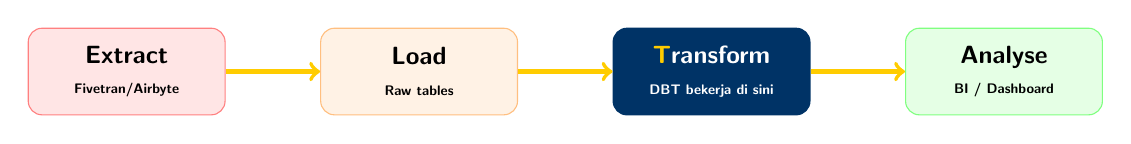
\begin{tikzpicture}[
  box/.style={rectangle,draw=ugmblue,fill=blue!8,rounded corners=5pt,
    minimum width=2.5cm,minimum height=1.1cm,align=center,font=\small\bfseries},
  act/.style={rectangle,draw=ugmblue,fill=ugmblue,rounded corners=5pt,
    minimum width=2.5cm,minimum height=1.1cm,align=center,
    font=\small\bfseries,text=white},
  arr/.style={->,thick,color=ugmgold,line width=1.5pt}
]
  \node[box,fill=red!10,draw=red!50] (E)
    {Extract\\{\tiny Fivetran/Airbyte}};
  \node[box,fill=orange!10,draw=orange!50,right=1.2cm of E] (L)
    {Load\\{\tiny Raw tables}};
  \node[act,right=1.2cm of L] (T)
    {\textcolor{ugmgold}{T}ransform\\{\tiny \textbf{DBT} bekerja di sini}};
  \node[box,fill=green!10,draw=green!50,right=1.2cm of T] (A)
    {Analyse\\{\tiny BI / Dashboard}};
  \draw[arr] (E)--(L);
  \draw[arr] (L)--(T);
  \draw[arr] (T)--(A);
\end{tikzpicture}
\end{center}
DBT tidak mengekstrak atau memuat data---tugas tersebut dilakukan
oleh \textit{ingestion tool} seperti Fivetran atau Airbyte. DBT
hanya bekerja pada data yang sudah ada di dalam \textit{warehouse}
\citep{bi4all2024}. Pendekatan ini melahirkan peran baru bernama
\textbf{\textit{analytics engineer}}: menggabungkan keahlian SQL
seorang \textit{data analyst} dengan praktik rekayasa perangkat
lunak.
\subsubsection{Arsitektur Berlapis (\textit{Layered Architecture})}
 
Praktik terbaik dalam DBT menggunakan arsitektur berlapis yang
memisahkan tanggung jawab setiap tahap transformasi
\citep{dbtdoc}:
 
\begin{center}
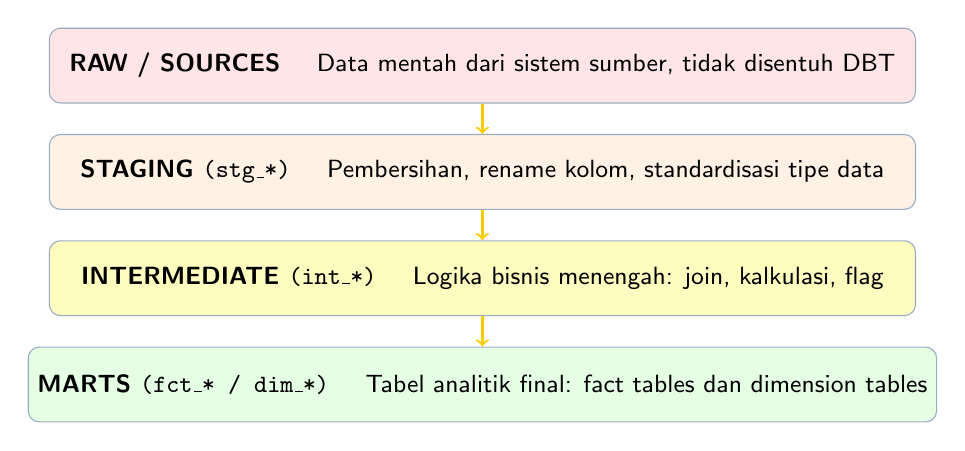
\begin{tikzpicture}[
  layer/.style={rectangle,draw=ugmblue!40,rounded corners=4pt,
    minimum width=11cm,minimum height=0.95cm,
    align=center,font=\small\bfseries},
  arr/.style={->,thick,color=ugmgold}
]
  \node[layer,fill=red!10] (raw) at (0,0)
    {RAW / SOURCES \quad
     {\normalfont\small Data mentah dari sistem sumber, tidak disentuh DBT}};
  \node[layer,fill=orange!10] (stg) at (0,-1.35)
    {STAGING \texttt{(stg\_*)} \quad
     {\normalfont\small Pembersihan, rename kolom, standardisasi tipe data}};
  \node[layer,fill=yellow!25] (int) at (0,-2.7)
    {INTERMEDIATE \texttt{(int\_*)} \quad
     {\normalfont\small Logika bisnis menengah: join, kalkulasi, flag}};
  \node[layer,fill=green!10] (mrt) at (0,-4.05)
    {MARTS \texttt{(fct\_* / dim\_*)} \quad
     {\normalfont\small Tabel analitik final: fact tables dan dimension tables}};
  \draw[arr] (raw)--(stg);
  \draw[arr] (stg)--(int);
  \draw[arr] (int)--(mrt);
\end{tikzpicture}
\end{center}

\section{Model dalam DBT dan Pemanfaatannya}
\subsection{Classic Model}
Pada modul ini digunakan database \textbf{ClassicModels} dari
MySQL Tutorial \citep{mysqltut} sebagai dataset eksplorasi.
ClassicModels adalah database peritel miniatur mobil klasik
yang menyediakan data bisnis nyata dengan relasi antar tabel
yang representatif untuk latihan membangun \textit{data warehouse}.

\begin{table}[H]
\centering
\caption{Delapan Tabel Sumber ClassicModels (OLTP)}
\begin{tabularx}{\linewidth}{llX}
\toprule
\textbf{Tabel} & \textbf{Baris} & \textbf{Deskripsi} \\
\midrule
\texttt{customers}    & 122   & Pelanggan: nama, kota, negara, \textit{credit limit} \\
\texttt{orders}       & 326   & Header pesanan: tanggal, status \\
\texttt{orderdetails} & 2.996 & Item pesanan: produk, kuantitas, harga satuan \\
\texttt{products}     & 110   & Katalog produk: nama, lini, vendor, harga \\
\texttt{productlines} & 7     & Lini produk: Classic Cars, Motorcycles, dll. \\
\texttt{employees}    & 23    & Karyawan dan struktur organisasi \\
\texttt{offices}      & 7     & Kantor penjualan: kota, negara, wilayah \\
\texttt{payments}     & 273   & Pembayaran pelanggan \\
\bottomrule
\end{tabularx}
\end{table}

Dari 8 tabel OLTP ini akan dibangun \textbf{star schema} dengan 5 tabel dimensi dan 2 tabel fakta menggunakan DBT\@.
\subsection{Struktur Model dalam DBT}
Dalam DBT, \textit{best practices} perancangan struktur model menggunakan arsitektur berlapis (\textit{layered architecture}) untuk memisahkan tanggung jawab dari setiap tahap transformasi. Pada implementasi proyek \texttt{classicmodels\_dbt}, strukturnya dibagi sebagai berikut:

% \subsection*{A. Direktori Project (\texttt{models/})}
DBT menyusun \textit{pipeline}-nya dalam folder \texttt{models/} yang mencakup dua subfolder utama, yaitu:

\begin{itemize}
    \item \textbf{Folder \texttt{staging/} (Layer Staging)} \\
    Layer ini bertujuan untuk melakukan standardisasi kolom, perbaikan tipe data, dan pembersihan awal dari \textit{raw data}. Model ini di-\textit{materialize} sebagai \textit{view}.
    \begin{itemize}
        \item Terdapat file konfigurasi \texttt{schema.yml} (untuk mendefinisikan sumber data dari OLTP asli beserta \textit{testing} dasar seperti \texttt{not\_null} atau \texttt{unique}).
        \item File-file SQL yang diberi prefiks \texttt{stg\_} (misalnya: \texttt{stg\_customers.sql}, \\
        \texttt{stg\_orders.sql}, \texttt{stg\_orderdetails.sql}, \texttt{stg\_products.sql}, \\
        \texttt{stg\_employees.sql}, \texttt{stg\_offices.sql}).
    \end{itemize}

    \item \textbf{Folder \texttt{marts/} (Layer Marts / Core)} \\
    Layer ini memuat struktur tabel analitik final yang menggabungkan logika bisnis dan menerapkan desain \textit{Star Schema} (\textit{Dimensional Modeling}). Tabel-tabel di sini di-\textit{materialize} sebagai tabel fisik di dalam database.
    \begin{itemize}
        \item File berprefiks \texttt{dim\_} (Tabel Dimensi / Konteks): \texttt{dim\_date.sql}, \\
        \texttt{dim\_product.sql}, \texttt{dim\_customer.sql}, \texttt{dim\_employee.sql}, \\
        \texttt{dim\_office.sql}.
        \item File berprefiks \texttt{fct\_} (Tabel Fakta / Pengukuran Bisnis): \\
        \texttt{fct\_sales.sql}, \texttt{fct\_monthly\_sales.sql}.
        \item File \texttt{schema.yml} untuk mengatur dokumentasi dan aturan \textit{testing} di level \textit{marts}.
    \end{itemize}
\end{itemize}

% \subsection*{B. Folder Pendukung Lainnya}
Selain folder \texttt{models/}, proyek ini juga memanfaatkan struktur komponen DBT lainnya:

\begin{itemize}
    \item \texttt{tests/}: Berisi \textit{custom SQL script} untuk pengujian logika bisnis spesifik (contohnya memastikan \textit{revenue} selalu positif, \texttt{assert\_revenue\_positive.sql}).
    \item \texttt{macros/}: Berisi fungsi \textit{reusable} dalam bahasa Jinja2 yang dipakai berulang dalam kode SQL (misalnya \texttt{revenue\_segment.sql}).
    \item \texttt{dbt\_project.yml}: Merupakan file konfigurasi induk yang mendefinisikan \textit{paths} (alur folder proyek) serta pengaturan \textit{materialization} di tiap layer.
\end{itemize}

\section{Data Quality dalam DBT}
% \section{Pengendalian Kualitas Data (\textit{Data Quality}) pada DBT}

Dalam perancangan \textit{Data Warehouse}, memastikan keakuratan dan integritas data adalah sebuah keharusan. DBT (\textit{Data Build Tool}) memfasilitasi kebutuhan ini melalui fitur \textbf{Pengujian Otomatis (\textit{Automated Testing})} yang terintegrasi secara mulus di dalam \textit{pipeline} transformasi data.

Konsep dasar pengujian di dalam DBT sangatlah sederhana: \textbf{sebuah tes adalah \textit{query} SQL (\texttt{SELECT}) yang secara khusus dirancang untuk menangkap data anomali atau data yang melanggar aturan}. Apabila \textit{query} tersebut tidak menemukan data yang salah (mengembalikan 0 baris), maka tes tersebut dinyatakan \textbf{lulus (\textit{pass})}. 

Secara umum, DBT membagi pengujian ke dalam dua pendekatan utama:

\subsection{Pengujian Bawaan (\textit{Generic Tests})}
\textit{Generic Tests} adalah sekumpulan fungsi pengujian standar bawaan DBT\@. Pengujian ini sangat praktis karena tidak perlu menulis kode SQL secara manual; cukup dengan mendeklarasikannya di dalam file konfigurasi (seperti \texttt{schema.yml})\@. 

Terdapat empat \textit{generic tests} utama yang sering digunakan di industri:
\begin{itemize}
    \item \textbf{\texttt{not\_null}}: Memvalidasi bahwa sebuah kolom wajib memiliki isi (tidak boleh \textit{null}).
    \item \textbf{\texttt{unique}}: Menjamin tidak ada nilai ganda (duplikat) di dalam sebuah kolom. Aturan ini sangat penting untuk memvalidasi kolom \textit{Primary Key}.
    \item \textbf{\texttt{accepted\_values}}: Membatasi nilai data agar hanya sesuai dengan daftar validasi yang telah ditetapkan (misalnya, kolom \textit{status} hanya boleh berisi nilai `Shipped', `Resolved', atau `Cancelled').
    \item \textbf{\texttt{relationships}}: Memverifikasi integritas referensial antar tabel (identik dengan konsep \textit{Foreign Key} pada \textit{relational database}).
\end{itemize}

\textbf{Contoh Pendefinisian di \texttt{schema.yml}:}
\begin{lstlisting}[caption=Konfigurasi Generic Test]
sources:
  - name: raw
    database: classicmodels
    tables:
      - name: orders
        columns:
          - name: orderNumber
            tests: 
              - not_null
              - unique
\end{lstlisting}

\subsection{Pengujian Logika Bisnis (\textit{Singular Tests})}
Dalam skenario dunia nyata, aturan bisnis seringkali lebih kompleks dari sekadar mengecek nilai kosong atau duplikat. Untuk mengatasi hal ini, DBT menyediakan \textit{Singular Tests}. 

Pada pendekatan ini, pengembang dapat menulis skrip SQL (\textit{custom query}) yang spesifik dan menyimpannya di dalam direktori \texttt{tests/}. Sebagai contoh, pada studi kasus \textbf{Classic Models}, kita harus memastikan bahwa perhitungan pendapatan (\textit{revenue}) tidak boleh bernilai negatif. 

\textbf{Contoh Skrip \texttt{tests/assert\_revenue\_positive.sql}:}
\begin{lstlisting}[caption=Skrip Singular Test]
-- Skrip ini dirancang untuk mendeteksi baris dengan pendapatan negatif.
-- Tes akan GAGAL jika ada output yang dihasilkan.
SELECT
    order_number,
    line_revenue
FROM {{ ref('fct_sales') }}
WHERE line_revenue < 0
\end{lstlisting}

\subsection{Menjalankan Pengujian (Eksekusi)}
Setelah semua aturan pengujian (\textit{generic} maupun \textit{singular}) didefinisikan, langkah terakhir adalah mengeksekusinya melalui antarmuka \textit{Command-Line} (CLI):
\begin{itemize}
    \item \texttt{dbt test}: Untuk menjalankan seluruh skrip pengujian saja.
    \item \texttt{dbt build}: Untuk menjalankan proses pembuatan tabel (\textit{run}) dan pengujian (\textit{test}) sekaligus dalam satu urutan kerja.
\end{itemize}

% \subsection*{Studi Kasus: Classic Models}
% Pada proyek pembelajaran Classic Models, implementasi arsitektur ini terbukti sangat efektif. \textit{Pipeline} yang dibangun berhasil memvalidasi seluruh logika dengan status \textbf{18/18 tes lulus (\textit{passed})}. Hal ini menjadi jaminan bahwa data telah bertransformasi dari sistem sumber (OLTP) ke dalam bentuk \textit{Star Schema} (\textit{Marts}) dengan tingkat akurasi dan kualitas yang tinggi.

\part{Analisis Kebutuhan Bisnis}
\chapter{Penyiapan Lingkungan DBT}
\begin{mybox}{Anggota kelompok}
\begin{enumerate}
    \itemsep0em
	\item ENGELBERTUS RANDE (NIM 25/573149/PPA/07211)
	\item GILBERT FANDILIAM MOOY (NIM 25/574767/PPA/07259)
	\item Sinta Siti Nuriah (NIM 25/575177/PPA/07274)
	\item Vicky Mahfudy (NIM 25/573019/PPA/07207)
\end{enumerate}
\end{mybox}

\section{DBT Core vs DBT Cloud}

\subsection{Definisi Dasar}

Dalam ekosistem transformasi data modern, dbt (\textit{data build tool}) hadir dalam dua varian utama yang melayani kebutuhan operasional yang berbeda:

\begin{enumerate}[leftmargin=*, labelsep=0.5em]
    \item \textbf{dbt Core:} Sekumpulan paket Python \textit{open-source}, yang dijalankan melalui baris perintah (\textit{command line}), yang membantu Anda mengubah, mendokumentasikan, dan menguji data Anda\cite{cook2023dbt}.
    \item \textbf{dbt Cloud:} Antarmuka pengguna (UI) berbasis web yang memungkinkan Anda untuk mengembangkan dan menerapkan \textit{pipeline} data yang dibangun di atas dbt Core\cite{cook2023dbt}.
\end{enumerate}

\subsection{Analisis Perbedaan}
Meskipun dbt Cloud menggunakan dbt Core sebagai mesin utamanya, terdapat beberapa perbedaan kunci dalam hal manajemen dan fungsionalitas:

\subsubsection{1. Deployment dan Manajemen Infrastruktur}
\begin{itemize}
    \item \textbf{dbt Core:} Mengharuskan pengguna untuk mengelola infrastruktur mereka sendiri (\textit{self-managed}). Sangat cocok bagi tim yang memiliki sumber daya DevOps untuk kendali penuh\cite{foundational2024dbt}.
    \item \textbf{dbt Cloud:} Merupakan layanan terkelola sepenuhnya (\textit{fully managed service})\cite{foundational2024dbt}. Hal ini mengurangi beban operasional karena dbt Labs menangani pembaruan dan stabilitas sistem\cite{foundational2024dbt}.
\end{itemize}

\subsubsection{2. Antarmuka Pengguna (User Interface)}
\begin{itemize}
    \item \textbf{dbt Core:} Beroperasi sepenuhnya melalui terminal/CLI, menuntut kemahiran dalam perintah-perintah teks\cite{foundational2024dbt}.
    \item \textbf{dbt Cloud:} Menyediakan IDE berbasis browser yang intuitif, menyederhanakan manajemen proyek bagi pengguna baru atau non-insinyur\cite{foundational2024dbt}.
\end{itemize}

\subsubsection{3. Biaya dan Skalabilitas}
\begin{itemize}
    \item \textbf{dbt Core:} Gratis untuk digunakan namun membutuhkan biaya operasional tersembunyi untuk pemeliharaan server dan implementasi fitur tambahan\cite{foundational2024dbt}.
    \item \textbf{dbt Cloud:} Berbasis langganan, namun sudah menyertakan fitur bawaan seperti penjadwalan (\textit{job scheduling}), pemantauan (\textit{monitoring}), dan peringatan (\textit{alerting}) yang siap pakai\citep{foundational2024dbt}.
\end{itemize}

\subsection{Ringkasan Perbandingan}

Setelah memahami detail fungsional dari masing-masing varian, tabel berikut menyajikan perbandingan parameter teknis secara berdampingan. Ringkasan ini bertujuan untuk mempermudah evaluasi pemilihan perangkat berdasarkan kebutuhan spesifik organisasi atau proyek:
 
\begin{table}[H]
\centering
\caption{Perbandingan DBT Core dan DBT Cloud}
\begin{tabularx}{\linewidth}{lXX}
\toprule
\textbf{Aspek} & \textbf{DBT Core} & \textbf{DBT Cloud} \\
\midrule
Lisensi      & Open source (gratis)      & SaaS berbayar (ada tier gratis) \\
Antarmuka    & \textit{Command line}     & Web IDE + GUI \\
Penjadwalan  & Perlu Airflow / Cron      & Built-in scheduler \\
Kolaborasi   & Via Git / GitHub          & Built-in collaboration \\
Dokumentasi  & Hosting mandiri           & Hosting otomatis \\
Rekomendasi  & Belajar, proyek lokal     & Tim produksi skala besar \\
Kontrol Versi & Konfigurasi Manual & Terintegrasi Langsung \\
Biaya Lisensi & Gratis & Berbayar (Berlangganan) \\ 
\bottomrule
\end{tabularx}
\end{table}



\subsection{Fitur dan Dukungan DBT}
DBT hadir dengan seperangkat fitur yang menjadikan transformasi data lebih terstruktur, andal, dan kolaboratif. Berikut adalah fitur-fitur utama beserta penjelasannya:
\subsubsection{Fitur: Models}
 
\textbf{Model} adalah unit kerja terkecil dalam DBT---satu file
\texttt{.sql} berisi satu pernyataan \texttt{SELECT}. Setiap model
menghasilkan satu tabel atau \textit{view} di database secara
otomatis. DBT mendukung empat jenis \textbf{materialisasi}:
 
\begin{itemize}[leftmargin=*,itemsep=3pt]
  \item \texttt{view} --- model dimaterialisasi sebagai
        \textit{database view}; tidak menyimpan data fisik.
        Cocok untuk lapisan \textit{staging}.
  \item \texttt{table} --- model dimaterialisasi sebagai tabel
        fisik di \textit{warehouse}. Cocok untuk lapisan
        \textit{marts} yang sering dikueri.
  \item \texttt{incremental} --- hanya memproses baris data baru
        sejak eksekusi terakhir. Sangat efisien untuk tabel besar
        yang terus bertambah.
  \item \texttt{ephemeral} --- tidak disimpan di database; kodenya
        disisipkan sebagai CTE ke dalam model yang mereferensikannya.
\end{itemize}

 \subsubsection{Fitur: Sources}
 
\textbf{Sources} adalah deklarasi tabel sumber (\textit{raw data})
yang sudah ada di \textit{warehouse}, dideklarasikan di file
\texttt{schema.yml} dengan fungsi \texttt{\{\{ source () \}\}}.
Manfaatnya: nama tabel sumber terpusat di satu tempat, dapat
dilengkapi \textit{freshness check}, dan otomatis terdokumentasi.
 
\subsubsection{Fitur: Tests}
 
DBT menyediakan pengujian data otomatis dalam dua bentuk:
 
\begin{enumerate}[leftmargin=*,itemsep=3pt]
  \item \textbf{Generic Tests} --- dikonfigurasi di
        \texttt{schema.yml}. Empat \textit{generic test} bawaan:
        \begin{itemize}[leftmargin=2em,itemsep=1pt]
          \item \texttt{not\_null} --- kolom tidak boleh NULL\@.
          \item \texttt{unique} --- setiap nilai harus unik.
          \item \texttt{accepted\_values} --- nilai dari daftar
                yang ditentukan.
          \item \texttt{relationships} --- integritas
                \textit{foreign key}.
        \end{itemize}
  \item \textbf{Singular Tests} --- file \texttt{.sql} kustom
        di folder \texttt{tests/}. Query menghasilkan baris
        \textit{hanya jika ada data yang gagal}; nol baris
        berarti \textit{pass}.
\end{enumerate}
 
\subsubsection{Fitur: Seeds, Snapshots, dan Macros}
 
\begin{itemize}[leftmargin=*,itemsep=4pt]
  \item \textbf{Seeds} --- file CSV kecil di folder \texttt{seeds/}
        yang di-\textit{upload} ke \textit{warehouse} via
        \texttt{dbt seed}. Cocok untuk data referensi statis
        seperti tabel pemetaan kode wilayah.
  \item \textbf{Snapshots} --- merekam riwayat perubahan data
        (\textit{Slowly Changing Dimensions}/SCD). Mendukung
        strategi \texttt{timestamp} dan \texttt{check}.
  \item \textbf{Macros} --- fungsi \textit{reusable} berbasis
        \textbf{Jinja2} yang dapat dipanggil di file SQL manapun.
        Paket komunitas \texttt{dbt\_utils} menyediakan
        ratusan macros siap pakai seperti
        \texttt{generate\_surrogate\_key ()} dan
        \texttt{date\_spine ()}.
\end{itemize}
\subsubsection{Fitur: Dokumentasi Otomatis}
 
Perintah \texttt{dbt docs generate} menghasilkan situs
dokumentasi interaktif yang mencakup:
\begin{itemize}[leftmargin=*,itemsep=2pt]
  \item \textbf{Model Catalog} --- semua model, kolom, tipe
        data, dan deskripsi.
  \item \textbf{DAG Lineage Graph} --- visualisasi interaktif
        alur transformasi dari \textit{raw sources} hingga
        tabel analitik final, termasuk \textit{column-level
        lineage}.
  \item \textbf{Source Freshness \& Test Coverage} --- laporan
        kesegaran data sumber dan cakupan pengujian per model.
\end{itemize}
\subsubsection{Dukungan Database (Adapters)}
 
Salah satu kekuatan DBT adalah dukungannya terhadap berbagai
\textit{data warehouse} melalui sistem \textbf{adapter}:
 
\begin{table}[H]
\centering
\caption{Adapter DBT yang Tersedia}
\begin{tabularx}{\linewidth}{llX}
\toprule
\textbf{Adapter} & \textbf{Instalasi} & \textbf{Keterangan} \\
\midrule
DuckDB     & \texttt{dbt-duckdb}     & In-process, ideal lokal/Colab \\
PostgreSQL & \texttt{dbt-postgres}   & Database relasional open source \\
BigQuery   & \texttt{dbt-bigquery}   & Google Cloud data warehouse \\
Snowflake  & \texttt{dbt-snowflake}  & Cloud data platform populer \\
Redshift   & \texttt{dbt-redshift}   & Amazon Web Services DWH \\
Databricks & \texttt{dbt-databricks} & Lakehouse platform \\
Spark      & \texttt{dbt-spark}      & Apache Spark engine \\
Trino      & \texttt{dbt-trino}      & Distributed query engine \\
\bottomrule
\end{tabularx}
\end{table}

\section{Instalasi \textit{Package}}
\subsection{Langkah 1: Instalasi DBT dan Pengaturan \textit{Base Path}}

Langkah awal dalam praktikum ini adalah menyiapkan lingkungan kerja di Google Colab, menginstal \textit{adapter} database yang diperlukan, serta memastikan persistensi data melalui Google Drive.

\subsubsection{Potongan Kode}
Berikut adalah skrip Python yang digunakan untuk inisialisasi lingkungan:

\begin{lstlisting}[language=Python, caption=Instalasi dan Konfigurasi Path]
# @title Step 1: Install DBT & Set Base Path
import os

# 1. Input Path dari User
root_path = "/content/drive/MyDrive"
folder_path = "dbt_analytics" 
base_folder_path = os.path.join(root_path, folder_path)

# 2. Instalasi dbt-duckdb
print("Sedang menginstal dbt-duckdb...")
!pip install -q dbt-duckdb

# 3. Mount Google Drive
from google.colab import drive
print("Menghubungkan ke Google Drive...")
drive.mount('/content/drive')

# 4. Membuat folder induk jika belum ada
if not os.path.exists(base_folder_path):
    os.makedirs(base_folder_path)
    print(f"Folder induk baru dibuat di: {base_folder_path}")
else:
    print(f"Folder induk ditemukan: {base_folder_path}")

# 5. Verifikasi Akhir
import duckdb
print(f"\nSiap! DuckDB v{duckdb.__version__} terpasang.")
\end{lstlisting}

\subsubsection{Penjelasan Potongan Kode}
\begin{itemize}
    \item \textbf{Baris 2\-7:} Menggunakan modul \texttt{os} untuk mendefinisikan jalur folder proyek (\texttt{base\_folder\_path}). Hal ini memungkinkan fleksibilitas bagi pengguna untuk menentukan nama folder penyimpanan di Google Drive.
    \item \textbf{Baris 10\-11:} Menginstal paket \texttt{dbt-duckdb}. Penggunaan parameter \texttt{-q} (\textit{quiet}) berfungsi untuk menyembunyikan log instalasi yang terlalu panjang.
    \item \textbf{Baris 14\-16:} Melakukan \textit{mounting} Google Drive ke \textit{filesystem} lokal Google Colab pada direktori \texttt{/content/drive}.
    \item \textbf{Baris 19\-23:} Memeriksa keberadaan folder proyek. Jika folder belum ada, sistem akan membuatnya secara otomatis menggunakan fungsi \texttt{os.makedirs}.
    \item \textbf{Baris 26\-27:} Melakukan verifikasi apakah \textit{library} DuckDB telah terinstal dengan benar dengan mencetak nomor versinya.
\end{itemize}

\subsubsection{Fungsi Kode}
Kode ini berfungsi sebagai \textbf{\textit{environment provisioner}}. Tujuannya adalah memastikan bahwa semua dependensi perangkat lunak tersedia, koneksi ke penyimpanan awan terjalin, dan struktur direktori siap digunakan sebelum proses transformasi data dimulai.

\subsubsection{Input dan Output}
\begin{itemize}
    \item \textbf{Input:} String \texttt{folder\_path} (nama folder proyek) dan kredensial akses Google Drive melalui proses autentikasi Colab.
    \item \textbf{Output:} Terpasangnya \textit{library} \texttt{dbt-duckdb}, direktori Google Drive yang terhubung, dan terciptanya folder \texttt{dbt\_analytics} di dalam Google Drive sebagai tempat penyimpanan permanen.
\end{itemize}

\subsubsection{Alasan Menggunakan Kode Tersebut}
Penggunaan kode ini sangat krusial karena Google Colab bersifat \textit{ephemeral} (sementara); data yang disimpan di \textit{local runtime} akan hilang setelah sesi berakhir. Dengan menghubungkan Google Drive dan mengatur \textit{base path} di sana, seluruh konfigurasi proyek dbt, file metadata, dan database DuckDB akan tersimpan secara permanen dan dapat diakses kembali di sesi berikutnya. Pemilihan \texttt{dbt-duckdb} didasarkan pada efisiensi DuckDB sebagai database analitik \textit{in-process} yang sangat cepat untuk lingkungan terbatas seperti Colab.

\subsection{Langkah 2: Inisialisasi Proyek DBT}

Setelah lingkungan dasar dan folder induk siap, langkah berikutnya adalah membentuk struktur direktori standar yang diperlukan oleh dbt untuk mengelola model, skrip, dan konfigurasi.

\subsubsection{Potongan Kode}
Berikut adalah kode yang digunakan untuk menginisialisasi proyek dbt:

\begin{lstlisting}[language=Python, caption=Inisialisasi Proyek DBT]
# @title Step 2: Setup Project DBT
# Masukkan nama project DBT yang akan Anda install.
project_name = "my_business_project" 

full_project_path = os.path.join(base_folder_path, project_name)

# Proses Inisialisasi
if not os.path.exists(full_project_path):
    os.chdir(base_folder_path)
    # Jalankan init tanpa tanya-tanya (skip-profile)
    !dbt init {project_name} --skip-profile-setup
    print(f"Project '{project_name}' berhasil dibuat di Drive!")
else:
    print(f"Project '{project_name}' sudah ada. Kami akan menggunakan folder yang tersedia.")

# Pindah ke direktori project
os.chdir(full_project_path)
print(f"Lokasi kerja saat ini: {os.getcwd()}")
\end{lstlisting}

\subsubsection{Penjelasan Potongan Kode}
\begin{itemize}
    \item \textbf{Baris 3\-5:} Mendefinisikan nama proyek (\texttt{project\_name}) dan menggabungkannya dengan \texttt{base\_folder\_path} untuk mendapatkan jalur lengkap direktori proyek.
    \item \textbf{Baris 8\-11:} Melakukan pengecekan apakah folder proyek sudah ada. Jika belum, skrip akan berpindah ke folder induk dan menjalankan perintah CLI \texttt{dbt init}. 
    \item \textbf{Parameter \texttt{--skip-profile-setup}:} Digunakan untuk melewati konfigurasi interaktif profil koneksi database. Hal ini penting dalam lingkungan otomatis seperti \textit{notebook} agar proses tidak terhenti menunggu input pengguna.
    \item \textbf{Baris 16\-17:} Mengubah direktori kerja aktif (\textit{working directory}) ke dalam folder proyek yang baru dibuat menggunakan \texttt{os.chdir}.
\end{itemize}

\subsubsection{Fungsi Kode}
Fungsi utama dari kode ini adalah \textbf{pembuatan kerangka proyek (\textit{scaffolding})}. Perintah \texttt{dbt init} secara otomatis menghasilkan folder-folder standar dbt seperti \texttt{models/}, \texttt{seeds/}, \texttt{snapshots/}, \texttt{macros/}, serta file konfigurasi utama \texttt{dbt\_project.yml}.

\subsubsection{Input dan Output}
\begin{itemize}
    \item \textbf{Input:} Variabel \texttt{project\_name} (nama proyek) dan variabel \texttt{base\_folder\_path} (lokasi penyimpanan induk dari langkah sebelumnya).
    \item \textbf{Output:} Terbentuknya struktur direktori dbt yang lengkap di Google Drive dan berpindahnya lokasi kerja sistem ke dalam folder tersebut.
\end{itemize}

\subsubsection{Alasan Menggunakan Kode Tersebut}
\begin{enumerate}
    \item \textbf{Standarisasi:} dbt mewajibkan struktur folder tertentu agar dapat mengenali model dan konfigurasi. Melakukan inisialisasi secara manual sangat rentan kesalahan, sehingga penggunaan \texttt{dbt init} adalah praktik terbaik.
    \item \textbf{Efisiensi Alur Kerja:} Dengan berpindah ke direktori proyek menggunakan \texttt{os.chdir}, perintah dbt selanjutnya (seperti \texttt{dbt run} atau \texttt{dbt seed}) dapat dijalankan langsung tanpa perlu menuliskan jalur folder secara berulang-ulang.
    \item \textbf{Idempotensi:} Pengecekan \texttt{if not os.path.exists} memastikan bahwa jika skrip dijalankan ulang, sistem tidak akan menimpa proyek yang sudah ada, melainkan hanya menyambungkan kembali sesi ke folder tersebut.
\end{enumerate}

\subsection{Langkah 3: Konfigurasi dan Pengujian Koneksi}

Setelah struktur proyek terbentuk, langkah krusial berikutnya adalah menghubungkan dbt dengan \textit{engine} database DuckDB\@. Hal ini dilakukan melalui pembuatan file konfigurasi \texttt{profiles.yml}.

\subsubsection{Potongan Kode}
Berikut adalah skrip Python yang digunakan untuk mengonfigurasi profil koneksi dan melakukan verifikasi:

\begin{lstlisting}[language=Python, caption=Konfigurasi profiles.yml dan Uji Koneksi]
# @title Step 3: Config & Connection Test
database_name = "my_business_db" 

# 1. VALIDASI DATA DARI STEP SEBELUMNYA
if 'full_project_path' not in locals() or 'project_name' not in locals():
    print("ERROR: Data project tidak ditemukan.")
else:
    # 2. KONFIGURASI FILE DATABASE
    if not database_name.endswith('.duckdb'):
        db_filename = database_name + ".duckdb"
    else:
        db_filename = database_name

    database_path = os.path.join(full_project_path, db_filename)

    # 3. PEMBUATAN PROFILES.YML
    profiles_content = f"""
{project_name}:
  outputs:
    dev:
      type: duckdb
      path: '{database_path}'
      extensions:
        - httpfs
        - parquet
      threads: 4
  target: dev
"""

    # Pastikan folder .dbt ada di home directory
    !mkdir -p /root/.dbt/

    with open('/root/.dbt/profiles.yml', 'w') as f:
        f.write(profiles_content)

    print(f"Konfigurasi tersimpan!")
    print(f"File database: {db_filename}")

    # 4. VERIFIKASI (dbt debug)
    print("Menjalankan dbt debug untuk mengecek koneksi...")
    os.chdir(full_project_path)
    !dbt debug
\end{lstlisting}

\subsubsection{Penjelasan Potongan Kode}
\begin{itemize}
    \item \textbf{Baris 5\-7:} Melakukan validasi variabel \texttt{full\_project\_path} dan \texttt{project\_name}. Hal ini menjamin bahwa langkah-langkah sebelumnya telah dijalankan dengan benar sebelum melakukan konfigurasi.
    \item \textbf{Baris 10\-15:} Logika untuk memastikan file database memiliki ekstensi \texttt{.duckdb}. Jalur lengkap database (\texttt{database\_path}) diletakkan di dalam folder proyek di Google Drive agar data bersifat permanen.
    \item \textbf{Baris 18\-29:} Membuat \textit{string} YAML yang mendefinisikan \texttt{profiles.yml}. Di sini ditentukan jenis database (\texttt{duckdb}), lokasi file, \textit{threads} untuk pemrosesan paralel, serta ekstensi tambahan (\texttt{httpfs} dan \texttt{parquet}) untuk kemampuan membaca data dari \textit{cloud storage}.
    \item \textbf{Baris 32\-35:} Membuat direktori tersembunyi \texttt{/root/.dbt/} dan menuliskan isi konfigurasi ke dalam file \texttt{profiles.yml}.
    \item \textbf{Baris 42\-44:} Menjalankan perintah CLI \texttt{dbt debug}. Perintah ini melakukan pemeriksaan sistem menyeluruh, mulai dari keberadaan file \texttt{dbt\_project.yml}, validitas \texttt{profiles.yml}, hingga koneksi fisik ke file database DuckDB\@.
\end{itemize}

\subsubsection{Fungsi Kode}
Kode ini berfungsi sebagai \textbf{jembatan penghubung (\textit{connectivity bridge})}. Dalam arsitektur dbt, proyek dbt (kode SQL) dan profil (koneksi database) dipisahkan secara logis. Kode ini secara dinamis membangun profil tersebut agar sesuai dengan lingkungan \textit{cloud} di Google Colab.

\subsubsection{Input dan Output}
\begin{itemize}
    \item \textbf{Input:} Nama database (\texttt{database\_name}) dari pengguna, serta jalur proyek yang sudah didefinisikan pada langkah sebelumnya.
    \item \textbf{Output:} File fisik \texttt{profiles.yml} di direktori sistem (\texttt{/root/.dbt/}) dan laporan status \texttt{dbt debug} yang menunjukkan status \texttt{OK CONNECTION} jika berhasil.
\end{itemize}

\subsubsection{Alasan Menggunakan Kode Tersebut}
\begin{enumerate}
    \item \textbf{Otomatisasi Lokasi Profil:} Secara \textit{default}, dbt mencari file profil di folder \texttt{~/.dbt/}. Karena kita bekerja di Google Colab yang berbasis Linux, skrip ini memastikan file tersebut dibuat di lokasi yang tepat secara otomatis tanpa perlu interaksi manual dengan editor teks.
    \item \textbf{Pemisahan Target:} Konfigurasi ini menggunakan target \texttt{dev}. Hal ini mempermudah jika di masa depan proyek dikembangkan ke tahap \texttt{prod} (produksi) dengan hanya mengganti profil tanpa mengubah kode model SQL\@.
    \item \textbf{Fitur Ekstensi DuckDB:} Penambahan ekstensi \texttt{httpfs} dan \texttt{parquet} dalam profil sangat penting untuk skenario data modern, di mana database sering kali harus berinteraksi dengan file eksternal yang disimpan di internet atau dalam format \textit{columnar}.
    \item \textbf{Diagnostik Dini:} Penggunaan \texttt{dbt debug} di akhir langkah instalasi sangat krusial untuk memastikan tidak ada kesalahan pengetikan (\textit{typo}) atau masalah hak akses sebelum pengguna mulai menulis kode transformasi yang kompleks.
\end{enumerate}
\section{Workflow dan Use Case}

Setelah infrastruktur dbt siap, proses dialihkan ke alur kerja pemrosesan data. Tahap pertama dalam alur kerja ini adalah \textit{Data Ingestion}, di mana data mentah dari sumber eksternal ditarik dan disiapkan ke dalam format yang dapat diproses oleh dbt.

\subsection{Langkah 4: Ingest Data SQL Mentah (\textit{Raw Data Ingestion})}

Langkah ini bertujuan untuk mengambil \textit{database dump} dalam format MySQL dan mengonversinya menjadi database DuckDB yang kompatibel.

\subsubsection{Potongan Kode}

\begin{lstlisting}[language=Python, caption=Fungsi Ingest SQL ke DuckDB]
# @title Step 4: Ingest Raw SQL Data
import requests
import re
import duckdb
import os

sql_url = "https://raw.githubusercontent.com/.../mysqlsampledatabase.sql"

def ingest_sql_to_duckdb(url, output_path):
    print(f"Mengunduh file dari: {url}...")
    response = requests.get(url)
    sql_content = response.content.decode('latin-1')

    print("Membersihkan sintaks MySQL...")
    # 1. Hapus komentar dan metadata MySQL
    sql_content = re.sub(r'/\*.*?\*/', '', sql_content, flags=re.DOTALL)
    
    # 2. Ganti backtick (`) ke kutip ganda (")
    sql_content = re.sub(r'`(\w+)`', r'"\1"', sql_content)

    # 3. Penyesuaian Tipe Data (MySQL -> DuckDB)
    sql_content = re.sub(r'(?i)\bmediumtext\b', 'TEXT', sql_content)
    sql_content = re.sub(r'(?i)\bint\(\d+\)', 'INTEGER', sql_content)

    # 4. Hapus engine-specific MySQL
    sql_content = re.sub(r'(?i)ENGINE=\w+', '', sql_content)
    
    # 5. Eksekusi ke DuckDB
    conn = duckdb.connect(output_path)
    statements = re.split(r';\s*\n', sql_content)
    for stmt in statements:
        if stmt.strip():
            conn.execute(stmt + ";")
    
    conn.close()

ingest_sql_to_duckdb(sql_url, database_path)
\end{lstlisting}

\subsubsection{Penjelasan Potongan Kode}
\begin{itemize}
    \item \textbf{Pengunduhan Data:} Menggunakan pustaka \texttt{requests} untuk mengambil file \texttt{.sql}. Penggunaan \textit{encoding} \texttt{latin-1} sangat penting karena dump database MySQL sering kali mengandung karakter non-UTF8.
    \item \textbf{Pembersihan Regex (Regular Expressions):} Karena DuckDB mengikuti standar ANSI SQL yang lebih ketat, skrip melakukan transformasi teks secara massal:
    \begin{itemize}
        \item Menghapus blok komentar (\texttt{/* ... */}).
        \item Mengganti \textit{backticks} (\`) dengan kutip ganda (\texttt{"}) agar nama tabel/kolom dapat dikenali oleh DuckDB.
        \item Mengonversi tipe data spesifik MySQL (seperti \texttt{mediumtext}) menjadi tipe generik \texttt{TEXT}.
    \end{itemize}
    \item \textbf{Pemisahan Statement:} Perintah SQL dipisah berdasarkan karakter titik koma (\texttt{;}) agar dapat dieksekusi satu per satu oleh \textit{engine} DuckDB melalui fungsi \texttt{conn.execute()}.
\end{itemize}

\subsubsection{Fungsi Kode}
Fungsi utama kode ini adalah sebagai \textbf{\textit{Source-to-Sink Transformer}}. Kode ini bertugas memigrasikan data dari format \textit{legacy} (MySQL dump) ke format \textit{modern analytical database} (DuckDB file) sambil melakukan normalisasi sintaks secara \textit{on-the-fly}.

\subsubsection{Input dan Output}
\begin{itemize}
    \item \textbf{Input:} URL publik yang mengarah ke file \texttt{.sql} (MySQL) dan jalur penyimpanan (\texttt{database\_path}) yang telah ditentukan pada langkah sebelumnya.
    \item \textbf{Output:} File database DuckDB (\texttt{.duckdb}) yang sudah terisi dengan tabel-tabel bisnis (seperti \texttt{customers}, \texttt{orders}, \texttt{products}) beserta datanya, siap untuk ditransformasikan oleh dbt.
\end{itemize}

\subsubsection{Alasan Menggunakan Kode Tersebut}
\begin{enumerate}
    \item \textbf{Inkompatibilitas Dialek:} Dialek MySQL memiliki banyak fitur non-standar (seperti \texttt{ENGINE=InnoDB} atau \texttt{KEY} tanpa nama) yang akan menyebabkan \textit{error} jika langsung dijalankan di DuckDB. Skrip ini memastikan proses transisi berjalan mulus tanpa intervensi manual.
    \item \textbf{Kecepatan Pemrosesan:} Melakukan pembersihan data menggunakan regex di memori (\textit{RAM}) jauh lebih cepat dibandingkan melakukan perbaikan manual pada file teks berukuran besar.
    \item \textbf{Integritas Data:} Dengan menghapus \textit{Foreign Key} dan \textit{Index} non-primer sementara pada saat \textit{ingestion}, kita menghindari masalah \textit{constraint violation} yang sering terjadi karena urutan \textit{insert} data dalam file dump yang tidak selalu berurutan.
\end{enumerate}

\subsection{Langkah 5: Pembuatan Model DBT Otomatis (\textit{YAML Model Generator})}

Setelah data mentah tersedia di DuckDB, tahap selanjutnya adalah menyusun struktur model dbt. Pada langkah ini, digunakan sebuah skrip generator berbasis YAML untuk membangun file \texttt{.sql} dan \texttt{.yml} secara otomatis ke dalam direktori proyek.

\subsubsection{Potongan Kode}

\begin{lstlisting}[language=Python, caption=DBT Model Generator dari YAML]
# @title Step 5: DBT Model Generator (YAML Version)
import requests
import os
import re
import yaml

config_url = "https://raw.githubusercontent.com/.../dbt_manifest.yml"

def setup_from_yaml(url):
    print(f"Mengunduh manifest YAML...")
    response = requests.get(url)
    file_map = yaml.safe_load(response.text)

    # Folder setup
    base_folders = ["models/staging", "models/dimensions", "models/marts"]
    for folder in base_folders:
        os.makedirs(os.path.join(full_project_path, folder), exist_ok=True)

    detected_sources = set()

    for rel_path, content in file_map.items():
        full_path = os.path.join(full_project_path, rel_path)
        os.makedirs(os.path.dirname(full_path), exist_ok=True)

        with open(full_path, "w") as f:
            f.write(content.strip())

        # Cari source mentah menggunakan Regex
        sources = re.findall(r"source\s*\(\s*['\"]main['\"]\s*,\s*['\"](\w+)['\"]\s*\)", content)
        for s in sources: detected_sources.add(s)
        print(f"   [Created] {rel_path}")

    # Generate sources.yml otomatis
    if detected_sources:
        source_tables = "\n".join([f"      - name: {t}" for t in sorted(detected_sources)])
        yaml_out = f"version: 2\nsources:\n  - name: main\n    tables:\n{source_tables}"
        with open(os.path.join(full_project_path, "models/staging/sources.yml"), "w") as f:
            f.write(yaml_out)

setup_from_yaml(config_url)
\end{lstlisting}

\subsubsection{Penjelasan Potongan Kode}
\begin{itemize}
    \item \textbf{Parsing Manifest:} Skrip menggunakan pustaka \texttt{PyYAML} untuk membaca file manifest eksternal. File ini berisi pemetaan antara jalur file (\textit{relative path}) dan isi logika SQL-nya.
    \item \textbf{Otomatisasi Direktori:} Kode secara otomatis membuat struktur folder \textit{Medallion Architecture} (\texttt{staging}, \texttt{dimensions}, \texttt{marts}) di dalam folder \texttt{models/}.
    \item \textbf{Ekstraksi \textit{Source} via Regex:} Skrip memindai setiap file SQL yang dibuat untuk mencari fungsi \texttt{source('main', '...')}. Nama tabel yang ditemukan dikumpulkan ke dalam sebuah \textit{set} untuk menghindari duplikasi.
    \item \textbf{Auto-Generation \texttt{sources.yml}:} Berdasarkan tabel-tabel yang terdeteksi, skrip menulis file \texttt{sources.yml}. File ini sangat penting bagi dbt untuk mengenali hubungan antara model \textit{staging} dengan tabel mentah di database.
\end{itemize}

\subsubsection{Fungsi Kode}
Fungsi utama kode ini adalah sebagai \textbf{\textit{Project Scaffolder}}. Dibandingkan membuat file SQL satu per satu secara manual, kode ini mengotomatiskan pembuatan seluruh arsitektur model data dbt hanya dari satu file konfigurasi terpusat.

\subsubsection{Input dan Output}
\begin{itemize}
    \item \textbf{Input:} URL ke file \texttt{dbt\_manifest.yml} yang berisi skema transformasi.
    \item \textbf{Output:} Terbentuknya puluhan file \texttt{.sql} di folder yang tepat serta satu file \texttt{sources.yml} yang telah terkonfigurasi secara otomatis di folder \texttt{staging}.
\end{itemize}

\subsubsection{Alasan Menggunakan Kode Tersebut}
\begin{enumerate}
    \item \textbf{Skalabilitas:} Dalam proyek data yang besar, membuat model \textit{staging} untuk puluhan tabel secara manual sangat memakan waktu. Otomatisasi ini mempercepat proses \textit{development}.
    \item \textbf{Konsistensi Struktur:} Dengan menggunakan generator, penamaan folder dan file akan selalu mengikuti standar yang sama, mengurangi risiko \textit{broken references} antar model.
    \item \textbf{Sinkronisasi \textit{Source}:} Fitur ekstraksi \textit{source} otomatis memastikan bahwa setiap tabel mentah yang dipanggil di model SQL pasti terdaftar di \texttt{sources.yml}. Jika tidak terdaftar, perintah \texttt{dbt run} akan gagal.
\end{enumerate}

\subsection{Langkah 6: Eksekusi Model dbt (\textit{dbt Run})}

Pada tahap ini, dbt melakukan orkestrasi transformasi data. Kode SQL yang bersifat deklaratif pada folder \texttt{models/} dieksekusi untuk membentuk tabel atau \textit{view} nyata di dalam database DuckDB.

\subsubsection{Potongan Kode}
Berikut adalah perintah CLI yang dijalankan untuk memproses transformasi data secara bertahap:

\begin{lstlisting}[language=Python, caption=Eksekusi Bertahap Model dbt]
# @title Step 6: Run dbt Models
%cd {full_project_path}

# Menjalankan transformasi secara modular
!dbt run --select staging
!dbt run --select dimensions
!dbt run --select marts
\end{lstlisting}

\subsubsection{Penjelasan Potongan Kode}
\begin{itemize}
    \item \textbf{\texttt{\%cd \{full\_project\_path\}}:} Memastikan \textit{environment} berada di direktori akar proyek dbt. Perintah dbt hanya dapat berjalan jika ia menemukan file \texttt{dbt\_project.yml} di direktori aktif.
    \item \textbf{\texttt{--select staging}:} Memerintahkan dbt untuk hanya mengeksekusi model yang berada di folder \texttt{staging}. Ini adalah lapisan pertama (\textit{Bronze Layer}) yang membersihkan data mentah.
    \item \textbf{\texttt{--select dimensions}:} Mengeksekusi lapisan kedua (\textit{Silver Layer}) yang berisi tabel dimensi hasil denormalisasi data staging.
    \item \textbf{\texttt{--select marts}:} Mengeksekusi lapisan terakhir (\textit{Gold Layer}) yang berisi tabel fakta atau metrik bisnis yang siap dikonsumsi oleh alat visualisasi atau laporan.
\end{itemize}

\subsubsection{Fungsi Kode}
Fungsi utama dari kode ini adalah sebagai \textbf{\textit{Orchestrator}}. dbt tidak hanya menjalankan SQL, tetapi juga menangani \textit{Dependency Management}. dbt memahami tabel mana yang harus dibuat lebih dulu berdasarkan referensi fungsi \texttt{ref()} yang ada di dalam skrip SQL.

\subsubsection{Input dan Output}
\begin{itemize}
    \item \textbf{Input:} File \texttt{.sql} dalam folder \texttt{models/}, konfigurasi \texttt{profiles.yml}, dan data mentah dalam file \texttt{.duckdb}.
    \item \textbf{Output:} Terbentuknya objek-objek database (Tabel dan \textit{View}) di dalam DuckDB. Log konsol akan menampilkan status tiap model (misalnya: \texttt{OK created view model.staging.stg\_orders}).
\end{itemize}

\subsubsection{Alasan Menggunakan Kode Tersebut}
\begin{enumerate}
    \item \textbf{Implementasi Medallion Architecture:} Dengan menggunakan \textit{flag} \texttt{--select}, kita memastikan alur data berjalan searah dari yang paling mentah hingga paling matang. Hal ini memudahkan isolasi jika terjadi \textit{error} pada salah satu lapisan.
    \item \textbf{Efisiensi Waktu dan Sumber Daya:} Jika kita melakukan perubahan hanya pada folder \texttt{marts}, kita tidak perlu menjalankan ulang seluruh proyek. Cukup gunakan seleksi folder untuk memperbarui bagian yang relevan.
    \item \textbf{Abstraksi DDL:} Pengguna tidak perlu menulis perintah \texttt{CREATE TABLE} atau \texttt{DROP TABLE} secara manual. dbt menangani \textit{Data Definition Language} (DDL) secara otomatis di balik layar, sehingga analis bisa fokus sepenuhnya pada logika transformasi.
\end{enumerate}

\subsection{Langkah 7: Verifikasi Data dan Analisis Hasil (\textit{Data Checking})}

Setelah siklus transformasi dbt selesai, tahap krusial berikutnya adalah melakukan verifikasi terhadap data yang dihasilkan. Langkah ini memastikan bahwa tabel fakta (\textit{fact tables}) dan dimensi yang dibuat telah berisi data yang akurat dan siap untuk dianalisis.

\subsubsection{Potongan Kode}
Berikut adalah fungsi Python yang digunakan untuk melakukan kueri langsung ke database DuckDB dan menampilkan hasilnya dalam format tabular:

\begin{lstlisting}[language=Python, caption=Verifikasi Hasil Transformasi dengan Python]
# @title Step 7: Data Checking
import duckdb
import pandas as pd

# Query kustom untuk mengecek hasil
user_query = "SELECT * FROM fct_order_lines LIMIT 5" 

def run_custom_query(query):
    conn = duckdb.connect(database_path)
    try:
        print(f"Executing: {query}")
        # Mengonversi hasil kueri langsung ke Pandas DataFrame
        df = conn.execute(query).df()
        if df.empty:
            print("Query berhasil tapi tidak ada data yang ditemukan.")
        else:
            display(df)
    except Exception as e:
        print(f"Query Error: {e}")
    finally:
        conn.close()

run_custom_query(user_query)
\end{lstlisting}

\subsubsection{Penjelasan Potongan Kode}
\begin{itemize}
    \item \textbf{Integrasi DuckDB dan Pandas:} Skrip ini memanfaatkan kemampuan DuckDB untuk mengekspor hasil kueri secara langsung ke dalam objek \texttt{DataFrame} milik \textit{library} Pandas menggunakan fungsi \texttt{.df()}.
    \item \textbf{Manajemen Koneksi:} Kode menggunakan blok \texttt{try...except...finally} untuk memastikan bahwa koneksi ke database (\texttt{conn.close()}) selalu ditutup, baik kueri berhasil maupun gagal. Hal ini mencegah terjadinya \textit{database lock} yang sering terjadi pada database berbasis file.
    \item \textbf{\texttt{display(df)}:} Menggunakan fungsi tampilan interaktif Google Colab untuk menyajikan data dalam bentuk tabel yang mudah dibaca oleh manusia dibandingkan teks mentah.
\end{itemize}

\subsubsection{Fungsi Kode}
Fungsi utama kode ini adalah sebagai \textbf{Alat Validasi dan Eksplorasi (\textit{Validation and Exploration Tool})}. Kode ini bertindak sebagai jembatan antara lapisan penyimpanan data (DuckDB) dengan lapisan presentasi (Pandas/Colab), memungkinkan pengembang untuk mengintip isi tabel hasil olahan dbt secara instan.

\subsubsection{Input dan Output}
\begin{itemize}
    \item \textbf{Input:} \textit{String} kueri SQL standar (misalnya kueri ke tabel \texttt{fct\_order\_lines} atau \texttt{dim\_customer}).
    \item \textbf{Output:} Tabel interaktif yang menampilkan kolom dan baris data hasil transformasi, atau pesan kesalahan jika sintaks SQL salah atau tabel belum terbentuk.
\end{itemize}

\subsubsection{Alasan Menggunakan Kode Tersebut}
\begin{enumerate}
    \item \textbf{Umpan Balik Cepat (\textit{Fast Feedback Loop}):} Sebelum dokumen laporan resmi dibuat, analis perlu memastikan tidak ada nilai \texttt{NULL} pada kolom kunci atau kesalahan perhitungan metrik. Menjalankan kueri SQL singkat adalah cara tercepat untuk melakukan hal tersebut.
    \item \textbf{Kesiapan Analitik:} Dengan mengonversi data ke Pandas DataFrame, kode ini secara teknis telah menyiapkan data untuk proses selanjutnya, seperti pembuatan grafik menggunakan \textit{Matplotlib} atau \textit{Seaborn} yang ada di dalam ekosistem Python.
    \item \textbf{Transparansi Model:} Memungkinkan pengguna untuk melihat bagaimana data mentah yang di-\textit{ingest} pada Langkah 4 telah berubah bentuk secara signifikan menjadi informasi bisnis yang terstruktur setelah melewati Langkah 6.
\end{enumerate}

\subsection{Langkah 8: Eksplorasi Wawasan Bisnis (\textit{Business Insight Exploration})}

Setelah data berhasil ditransformasi dan divalidasi, langkah terakhir dalam alur kerja ini adalah melakukan kueri analitik untuk mengekstraksi wawasan bisnis. Pada tahap ini, data yang tersebar di berbagai tabel dihubungkan untuk menghitung metrik seperti pendapatan, keuntungan, dan margin.

\subsubsection{Potongan Kode}
Berikut adalah kode yang digunakan untuk menghasilkan tabel laporan performa produk:

\begin{lstlisting}[language=Python, caption=Eksplorasi Insight Bisnis dengan SQL dan Pandas]
# @title Step 8: Explore Business Insight
import duckdb
import pandas as pd

# Query untuk analisis Revenue dan Margin per Lini Produk
insight_query = """
SELECT 
    p.product_line, 
    ROUND(SUM(f.quantity_ordered * f.price_each), 2) as total_revenue, 
    ROUND(SUM(f.quantity_ordered * (f.price_each - p.buy_price)), 2) as total_profit, 
    ROUND((SUM(f.quantity_ordered * (f.price_each - p.buy_price)) / 
           SUM(f.quantity_ordered * f.price_each)) * 100, 2) as margin_pct 
FROM fct_order_lines f 
JOIN stg_products p ON f.product_code = p.product_code 
GROUP BY 1 
ORDER BY total_revenue DESC
"""

def run_insight_table(query):
    conn = duckdb.connect(database_path)
    try:
        print("Menghasilkan Tabel Insight Bisnis...")
        df = conn.execute(query).df()

        if df.empty:
            print("Tidak ada data yang ditemukan.")
        else:
            # Mengatur format angka agar mudah dibaca
            pd.options.display.float_format = '{:,.2f}'.format
            display(df)
    except Exception as e:
        print(f"Error pada Query: {e}")
    finally:
        conn.close()

run_insight_table(insight_query)
\end{lstlisting}

\subsubsection{Penjelasan Potongan Kode}
\begin{itemize}
    \item \textbf{Logika Bisnis SQL (Baris 7-19):} Kueri ini melakukan operasi JOIN antara tabel fakta \texttt{fct\_order\_lines} (berisi transaksi) dan tabel staging \texttt{stg\_products} (berisi harga beli dasar). Di sini dilakukan kalkulasi metrik finansial:
    \begin{itemize}
        \item \textit{Total Revenue}: Perkalian jumlah pesanan dengan harga jual.
        \item \textit{Total Profit}: Selisih antara harga jual dan harga beli dikalikan jumlah pesanan.
        \item \textit{Margin \%}: Persentase profit terhadap total pendapatan.
    \end{itemize}
    \item \textbf{Pemformatan Data (Baris 29):} Menggunakan \texttt{pd.options.display.float\_format} untuk menambahkan pemisah ribuan (koma) dan membatasi dua angka di belakang desimal. Hal ini sangat penting untuk penyajian data finansial agar lebih profesional dan mudah dibaca.
    \item \textbf{Grup dan Urutan:} Mengelompokkan data berdasarkan lini produk (\texttt{GROUP BY 1}) dan mengurutkannya dari pendapatan tertinggi ke terendah.
\end{itemize}

\subsubsection{Fungsi Kode}
Fungsi utama kode ini adalah sebagai \textbf{Lapisan Penyajian Informasi (\textit{Information Delivery Layer})}. Kode ini mengubah data terstruktur yang dihasilkan oleh dbt menjadi laporan eksekutif yang siap digunakan oleh manajer atau pemilik bisnis untuk mengambil keputusan strategis.

\subsubsection{Input dan Output}
\begin{itemize}
    \item \textbf{Input:} Kueri SQL agregasi yang kompleks dan akses ke file database \texttt{.duckdb}.
    \item \textbf{Output:} Laporan performa lini produk yang berisi kolom \texttt{product\_line}, \texttt{total\_revenue}, \texttt{total\_profit}, dan \texttt{margin\_pct}.
\end{itemize}

\subsubsection{Alasan Menggunakan Kode Tersebut}
\begin{enumerate}
    \item \textbf{Demonstrasi Nilai dbt:} Kode ini membuktikan bahwa arsitektur tabel fakta dan dimensi yang dibangun dengan dbt dapat memudahkan penulisan kueri yang kompleks menjadi lebih sederhana dan efisien.
    \item \textbf{Decision Making}: Dengan mengetahui margin per lini produk (misalnya membandingkan \textit{Classic Cars} dengan \textit{Vintage Cars}), perusahaan dapat menentukan produk mana yang paling menguntungkan, bukan hanya yang memiliki omzet besar.
    \item \textbf{Fleksibilitas Analitik:} Dengan menggunakan Pandas di dalam Google Colab, pengguna dapat dengan cepat mengubah parameter kueri atau bahkan menambahkan visualisasi grafik setelah tabel ditampilkan.
\end{enumerate}

\subsection{Langkah 9: Dokumentasi Otomatis dan Silsilah Data (\textit{dbt Docs})}

Tahap akhir dari siklus pengembangan dbt adalah pembuatan dokumentasi. dbt memiliki kemampuan unik untuk menghasilkan situs web statis yang mendokumentasikan setiap model, kolom, dan hubungan antar tabel secara otomatis.

\subsubsection{Potongan Kode}
Berikut adalah perintah untuk memproduksi dan menampilkan dokumentasi di lingkungan Google Colab:

\begin{lstlisting}[language=Python, caption=Generasi Dokumentasi dan Lineage Graph]
# @title Step 9: Generate dbt Docs
# 1. Menghasilkan file metadata dokumentasi
!dbt docs generate

from google.colab import output
# 2. Forward port agar bisa diakses dari browser luar
output.serve_kernel_port_as_window(8088)

# 3. Menjalankan server dokumentasi
!dbt docs serve --port 8088
\end{lstlisting}

\subsubsection{Penjelasan Potongan Kode}
\begin{itemize}
    \item \textbf{\texttt{dbt docs generate}:} Instruksi ini memerintahkan dbt untuk memindai seluruh proyek dan database untuk menghasilkan file \texttt{manifest.json} dan \texttt{catalog.json}. File-file ini berisi informasi lengkap mengenai skema, tipe data, dan dependensi antar model.
    \item \textbf{\texttt{output.serve\_kernel\_port\_as\_window(8088)}:} Karena Google Colab berjalan di mesin virtual terisolasi, port lokal tidak bisa diakses langsung. Fungsi ini melakukan \textit{port forwarding} agar server dokumentasi dapat dibuka di tab browser baru pengguna.
    \item \textbf{\texttt{dbt docs serve --port 8088}:} Menjalankan server web ringan yang menyajikan antarmuka visual dokumentasi dbt melalui port 8088.
\end{itemize}

\subsubsection{Fungsi Kode}
Fungsi utama kode ini adalah sebagai \textbf{Sistem Katalog Data Otomatis}. Kode ini menghilangkan kebutuhan untuk menulis dokumentasi manual di dokumen terpisah. Paling penting, dbt menghasilkan \textit{Lineage Graph} yang memvisualisasikan aliran data dari sumber (\textit{source}) menuju \textit{staging}, kemudian ke \textit{dimension}, hingga berakhir di \textit{marts}.

\subsubsection{Input dan Output}
\begin{itemize}
    \item \textbf{Input:} Metadata proyek dalam folder \texttt{target/} dan skema database DuckDB.
    \item \textbf{Output:} Sebuah situs web interaktif yang menampilkan deskripsi tabel, daftar kolom, tipe data, kode SQL sumber, dan grafik silsilah data (*Lineage Graph*).
\end{itemize}

\subsubsection{Alasan Menggunakan Kode Tersebut}
\begin{enumerate}
    \item \textbf{Transparansi Data:} Dengan \textit{Lineage Graph}, analis dapat dengan mudah melacak dari mana sebuah angka di laporan berasal. Jika terjadi kesalahan pada tabel fakta, analis dapat melihat tabel \textit{staging} mana yang menjadi sumber masalahnya.
    \item \textbf{Kemudahan Audit:} Dokumentasi ini mencakup skrip SQL asli yang membentuk setiap tabel, sehingga memudahkan auditor atau rekan tim lainnya untuk meninjau logika transformasi tanpa harus membuka file kode satu per satu.
    \item \textbf{Efisiensi Komunikasi:} Dokumentasi ini berfungsi sebagai \textit{single source of truth} bagi tim data dan pemangku kepentingan bisnis untuk memahami definisi data yang digunakan dalam organisasi.
\end{enumerate}

\part{Perancangan Dimensional Modeling}
\chapter{Studi Kasus dan Pembahasan}

\begin{mybox}{Anggota kelompok}
	\begin{enumerate}
		\itemsep0em
		\item ENGELBERTUS RANDE (NIM 25/573149/PPA/07211)
		\item GILBERT FANDILIAM MOOY (NIM 25/574767/PPA/07259)
		\item Sinta Siti Nuriah (NIM 25/575177/PPA/07274)
		\item Vicky Mahfudy (NIM 25/573019/PPA/07207)
	\end{enumerate}
\end{mybox}

\section{Skema Data Base \& Data Warehouse}

Skema pada sistem *Data Warehouse* ini menggunakan dataset \textit{ClassicModels}. Data bersumber dari *dump file* MySQL yang berisi rekam jejak sistem OLTP dan diubah ke dalam bentuk OLAP menggunakan DuckDB. Tabel yang dihasilkan meliputi tabel dimensi dan fakta seperti rincian pelanggan, produk, transaksi pesanan, dan pembayaran.

\begin{table}[H]
	\centering
	\caption{Ringkasan Baris Tabel pada DuckDB}
	\begin{tabularx}{0.7\textwidth}{@{} X r @{}}
		\toprule
		\textbf{Nama Tabel} & \textbf{Jumlah Baris (Rows)} \\ \midrule
		customers & 122 \\
		employees & 23 \\
		offices & 7 \\
		orderdetails & 2.996 \\
		orders & 326 \\
		payments & 273 \\
		productlines & 7 \\
		products & 110 \\ \bottomrule
	\end{tabularx}
\end{table}

\section{Skenario dan Penyelesaian}

Berikut adalah langkah-langkah detail implementasi yang dieksekusi secara berurutan melalui lingkungan komputasi \textit{Jupyter Notebook} di Google Colab.

\subsection{Background and Setup}
Langkah awal ini berfokus pada persiapan lingkungan kerja dengan menginstal alat pemodelan data (dbt) dan sistem basis data (DuckDB), serta memastikan semuanya berada pada versi yang sesuai.

\begin{lstlisting}[language=bash, numbers=left, caption={Instalasi Library}]
	!pip install dbt-core dbt-duckdb duckdb pandas
\end{lstlisting}

\begin{lstlisting}[language=bash, numbers=left, caption={Output: Log Instalasi (Singkat)}]
	Collecting dbt-core
	Downloading dbt_core-1.11.8-py3-none-any.whl.metadata (4.4 kB)
	Collecting dbt-duckdb
	Downloading dbt_duckdb-1.10.1-py3-none-any.whl.metadata (38 kB)
	Requirement already satisfied: duckdb in /usr/local/lib/python3.12/dist-packages (1.3.2)
	Requirement already satisfied: pandas in /usr/local/lib/python3.12/dist-packages (2.2.2)
	...
	Successfully installed agate-1.9.1 colorama-0.4.6 daff-1.4.2 dbt-adapters-1.22.10 dbt-common-1.38.0 dbt-core-1.11.8 dbt-duckdb-1.10.1 ...
\end{lstlisting}

\begin{lstlisting}[language=bash, numbers=left, caption={Verifikasi Versi dbt}]
	!dbt --version
\end{lstlisting}

\begin{lstlisting}[language=bash, numbers=left, caption={Output: Versi dbt}]
	Core:
	- installed: 1.11.8
	- latest:    1.11.8 - Up to date!
	
	Plugins:
	- duckdb: 1.10.1 - Up to date!
\end{lstlisting}

\begin{lstlisting}[language=Python, numbers=left, caption={Verifikasi Versi DuckDB}]
	!python -c "import duckdb; print(duckdb.__version__)"
	# Output:
	# 1.3.2
\end{lstlisting}

\begin{lstlisting}[language=Python, numbers=left, caption={Koneksi ke Google Drive}]
	from google.colab import drive
	drive.mount('/content/drive')
	# Output: Drive already mounted at /content/drive...
\end{lstlisting}

\subsection{Convert MySQL to DuckDB}
Data asli berada dalam format file *dump* SQL yang memiliki sintaks spesifik MySQL. Proses ini akan membersihkan sintaks tersebut (misalnya, menghapus parameter \textit{ENGINE}, mengubah *backticks*, dan merapikan klausa \textit{FOREIGN KEY}) agar kompatibel untuk dieksekusi di DuckDB.
\clearpage
\begin{lstlisting}[language=Python, numbers=left, caption={Konfigurasi Path}]
	import os
	# --- PENGATURAN PATH GOOGLE DRIVE ---
	DRIVE_BASE = "/content/drive/MyDrive/Term 1/Data Warehouse/Tugas DBT"
	INPUT_FILE = DRIVE_BASE+"/mysqlsampledatabase.sql"
	DUCKDB_FILE = DRIVE_BASE+"/classicmodels.duckdb"
	OUTPUT_FILE = os.path.join(DUCKDB_FILE)
\end{lstlisting}

\begin{lstlisting}[language=Python, numbers=left, caption={Script ETL: Pembersihan dan Ingesti SQL}]
	import re
	import duckdb
	from google.colab import drive
	
	# 1. Mount Google Drive
	drive.mount('/content/drive')
	
	def convert_mysql_to_duckdb(input_sql_path, output_duckdb_path):
	if not os.path.exists(input_sql_path):
	print(f"File {input_sql_path} tidak ditemukan!")
	return
	
	print(f"Membaca file: {input_sql_path}...")
	with open(input_sql_path, 'r', encoding='latin-1') as f:
	sql_content = f.read()
	
	print("Membersihkan sintaks MySQL...")
	
	# 1. Hapus komentar dan metadata MySQL level database
	sql_content = re.sub(r'/\*.*?\*/', '', sql_content, flags=re.DOTALL)
	sql_content = re.sub(r'--.*?\n', '\n', sql_content)
	sql_content = re.sub(r'(?i)CREATE DATABASE.*?;', '', sql_content)
	sql_content = re.sub(r'(?i)USE\s+\w+;', '', sql_content)
	
	# 2. FIX KOLOM & TABEL (Penting untuk addressLine1, dsb)
	sql_content = re.sub(r'`(\w+)`', r'"\1"', sql_content)
	
	# 3. Sesuaikan tipe data
	sql_content = re.sub(r'(?i)\bmediumtext\b', 'TEXT', sql_content)
	sql_content = re.sub(r'(?i)\bmediumblob\b', 'BLOB', sql_content)
	sql_content = re.sub(r'(?i)\bsmallint\(\d+\)', 'SMALLINT', sql_content)
	sql_content = re.sub(r'(?i)\bint\(\d+\)', 'INTEGER', sql_content)
	
	# 4. Perbaiki Escape Characters & Tanggal
	sql_content = sql_content.replace(r"\'", "''")
	sql_content = sql_content.replace("'0000-00-00'", "NULL")
	
	# 5. Hapus engine-specific MySQL
	sql_content = re.sub(r'(?i)ENGINE=\w+', '', sql_content)
	sql_content = re.sub(r'(?i)DEFAULT CHARSET=\w+', '', sql_content)
	sql_content = re.sub(r'(?i)COLLATE=\w+', '', sql_content)
	
	# 6. Hapus baris FOREIGN KEY
	lines = sql_content.split('\n')
	cleaned_lines = []
	for line in lines:
	if 'FOREIGN KEY' in line.upper(): continue
	if 'KEY ' in line.upper() and 'PRIMARY' not in line.upper(): continue
	cleaned_lines.append(line)
	
	sql_content = '\n'.join(cleaned_lines)
	
	# 7. Bersihkan koma gantung (dangling comma)
	sql_content = re.sub(r',\s*\)', '\n)', sql_content)
	
	# --- PROSES EKSEKUSI ---
	if os.path.exists(output_duckdb_path):
	os.remove(output_duckdb_path)
	
	print(f"Mengeksekusi ke DuckDB di: {output_duckdb_path}")
	conn = duckdb.connect(output_duckdb_path)
	statements = re.split(r';\s*\n', sql_content)
	
	success_count = 0
	error_count = 0
	
	for stmt in statements:
	clean_stmt = stmt.strip()
	if clean_stmt:
	try:
	conn.execute(clean_stmt + ";")
	success_count += 1
	except Exception as e:
	if "DROP" not in clean_stmt.upper():
	print(f"Warning pada: {clean_stmt[:50]}... \n Detail: {e}")
	error_count += 1
	
	print(f"\nSelesai! Berhasil: {success_count}, Gagal: {error_count}")
	
	# Tampilkan Ringkasan Tabel
	print("\n" + "="*40)
	print(f"{'TABEL':<20} | {'JUMLAH BARIS':>10}")
	print("-" * 40)
	try:
	tables = conn.execute("SHOW TABLES").fetchall()
	for (t,) in tables:
	count = conn.execute(f'SELECT COUNT(*) FROM "{t}"').fetchone()[0]
	print(f"{t:<20} | {count:>10}")
	except:
	pass
	conn.close()
	
	if __name__ == "__main__":
	if not os.path.exists(DRIVE_BASE):
	os.makedirs(DRIVE_BASE)
	convert_mysql_to_duckdb(INPUT_FILE, OUTPUT_FILE)
\end{lstlisting}

\begin{lstlisting}[language=bash, numbers=left, caption={Output: Hasil Eksekusi Pembuatan DuckDB}]
	Membaca file: /content/drive/MyDrive/Term 1/Data Warehouse/Tugas DBT/mysqlsampledatabase.sql...
	Membersihkan sintaks MySQL...
	Mengeksekusi ke DuckDB di: /content/drive/MyDrive/Term 1/Data Warehouse/Tugas DBT/classicmodels.duckdb
	
	Selesai! Berhasil: 24, Gagal: 0
	
	========================================
	TABEL                | JUMLAH BARIS
	----------------------------------------
	customers            |        122
	employees            |         23
	offices              |          7
	orderdetails         |       2996
	orders               |        326
	payments             |        273
	productlines         |          7
	products             |        110
\end{lstlisting}

Selanjutnya, dilakukan verifikasi skema pada \textit{schema main} dari objek \textit{database} DuckDB yang telah dibuat.

\begin{lstlisting}[language=Python, numbers=left, caption={Verifikasi Skema pada Data Warehouse}]
	## Pengecekan sampel dengan mengambil 3 baris
	
	# Buka koneksi ke file database yang sudah dikonversi
	con = duckdb.connect(DUCKDB_FILE)
	
	# -- 1. List all tables --------------------------------------------------------
	print("=" * 50)
	print("Source tables in 'main' schema")
	print("=" * 50)
	tables = con.execute("""
	SELECT table_name
	FROM   information_schema.tables
	WHERE  table_schema = 'main'
	ORDER  BY table_name
	""").fetchall()
	
	for (t,) in tables:
	print(f"  {t}")
	
	print(f"\nTotal: {len(tables)} tables")
	expected = {'customers', 'employees', 'offices', 'orderdetails',
		'orders', 'payments', 'productlines', 'products'}
	found = {t for (t,) in tables}
	missing = expected - found
	if missing:
	print(f"\n[WARN] Missing expected tables: {missing}")
	else:
	print("[OK] All 8 expected tables found.")
	
	# -- 2. Row counts per table ---------------------------------------------------
	print("\n" + "=" * 50)
	print("Row counts")
	print("=" * 50)
	for (t,) in tables:
	count = con.execute(f"SELECT COUNT(*) FROM {t}").fetchone()[0]
	print(f"  {t:<20} {count:>6} rows")
	
	# -- 3. Sample: first 3 rows of each table ------------------------------------
	print("\n" + "=" * 50)
	print("Sample rows (first 3 per table)")
	print("=" * 50)
	for (t,) in tables:
	print(f"\n-- {t} --")
	df = con.execute(f"SELECT * FROM {t} LIMIT 3").df()
	print(df.to_string(index=False))
	
	con.close()
\end{lstlisting}

\begin{lstlisting}[language=bash, numbers=left, caption={Output: Pengecekan sampel baris}]
	==================================================
	Source tables in 'main' schema
	==================================================
	customers
	employees
	offices
	orderdetails
	orders
	payments
	productlines
	products
	
	Total: 8 tables
	[OK] All 8 expected tables found.
	
	==================================================
	Row counts
	==================================================
	customers               122 rows
	employees                23 rows
	offices                   7 rows
	orderdetails           2996 rows
	orders                  326 rows
	payments                273 rows
	productlines              7 rows
	products                110 rows
	
	==================================================
	Sample rows (first 3 per table)
	==================================================
	
	-- customers --
	customerNumber               customerName contactLastName contactFirstName        phone      addressLine1 addressLine2      city    state postalCode   country  salesRepEmployeeNumber  creditLimit
	103          Atelier graphique         Schmitt          Carine    40.32.2555    54, rue Royale         None    Nantes     None      44000    France                    1370      21000.0
	112         Signal Gift Stores            King             Jean   7025551838   8489 Strong St.         None Las Vegas       NV      83030       USA                    1166      71800.0
	114 Australian Collectors, Co.        Ferguson            Peter 03 9520 4555 636 St Kilda Road      Level 3 Melbourne Victoria       3004 Australia                    1611     117300.0
	
	-- employees --
	employeeNumber  lastName firstName extension                          email officeCode  reportsTo     jobTitle
	1002    Murphy     Diane     x5800   dmurphy@classicmodelcars.com          1       <NA>    President
	1056 Patterson      Mary     x4611 mpatterso@classicmodelcars.com          1       1002     VP Sales
	1076  Firrelli      Jeff     x9273 jfirrelli@classicmodelcars.com          1       1002 VP Marketing
	
	-- offices --
	officeCode          city           phone         addressLine1 addressLine2 state country postalCode territory
	1 San Francisco +1 650 219 4782    100 Market Street    Suite 300    CA     USA      94080        NA
	2        Boston +1 215 837 0825     1550 Court Place    Suite 102    MA     USA      02107        NA
	3           NYC +1 212 555 3000 523 East 53rd Street      apt. 5A    NY     USA      10022        NA
	
	-- orderdetails --
	orderNumber productCode  quantityOrdered  priceEach  orderLineNumber
	10100    S18_1749               30     136.00                3
	10100    S18_2248               50      55.09                2
	10100    S18_4409               22      75.46                4
	
	-- orders --
	orderNumber  orderDate requiredDate shippedDate  status               comments  customerNumber
	10100 2003-01-06   2003-01-13  2003-01-10 Shipped                   None             363
	10101 2003-01-09   2003-01-18  2003-01-11 Shipped Check on availability.             128
	10102 2003-01-10   2003-01-18  2003-01-14 Shipped                   None             181
	
	-- payments --
	customerNumber checkNumber paymentDate   amount
	103    HQ336336  2004-10-19  6066.78
	103    JM555205  2003-06-05 14571.44
	103    OM314933  2004-12-18  1676.14
	
	-- productlines --
	productLine    textDescription                         htmlDescription image
	Classic Cars   Attention car enthusiasts...            None            <NA>
	Motorcycles    State-of-the-art replicas...            None            <NA>
	Planes         Diecast airplane replicas...            None            <NA>
	
	-- products --
	productCode productName                       productLine  stock buyPrice MSRP
	S10_1678    1969 Harley Davidson Chopper      Motorcycles  7933   48.81  95.70
	S10_1949    1952 Alpine Renault 1300          Classic Cars 7305   98.58 214.30
	S10_2016    1996 Moto Guzzi 1100i             Motorcycles  6625   68.99 118.94
\end{lstlisting}

\subsection{Working with dbt \& Profiles Configuration}
Untuk mengeksekusi model analitik, proyek dbt diinisialisasi dan diatur profil koneksinya agar merujuk ke file \textit{database} DuckDB (\texttt{classicmodels.duckdb}).

\begin{lstlisting}[language=Python, numbers=left, caption={Konfigurasi profiles.yml}]
	profiles_yaml = f"""
	classicmodels:
	target: dev
	outputs:
	dev:
	type: duckdb
	path: {DUCKDB_FILE}
	threads: 1
	"""
	with open("profiles.yml", "w") as f:
	f.write(profiles_yaml)
\end{lstlisting}

\section{Part 3: Building the Data Marts with dbt}

Bagian ini merupakan inti dari seluruh proses pemodelan data menggunakan dbt (\textit{data build tool}). Arsitektur yang dibangun mengikuti pola tiga lapisan (\textit{three-tier architecture}): \textit{Staging Layer} untuk pembersihan, \textit{Dimension Layer} untuk data master, dan \textit{Marts Layer} untuk tabel fakta.

\subsection{Step 1: Verify the Source Data}
Sebelum melakukan transformasi, dilakukan verifikasi integritas data pada \textit{Source Database}. Langkah ini memastikan bahwa tabel mentah telah terbaca dengan benar.

\begin{lstlisting}[language=Python, caption=Verifikasi Data Sumber]
# Preview relasi antara orders dan customers
results = conn.execute("""
    SELECT o.orderNumber, o.status, c.customerName
    FROM orders o
    JOIN customers c USING (customerNumber)
    LIMIT 3;
""").df()
print(results)
\end{lstlisting}

\textbf{Contoh Output:}
\begin{verbatim}
   orderNumber    status             customerName
0        10100   Shipped      Online Diecast Creations
1        10101   Shipped          Blauer See Auto, Co.
2        10102   Shipped             Vitachrome Inc.
\end{verbatim}

\subsection{Step 2: Build the Staging Layer}
\textit{Staging layer} melakukan standarisasi nama kolom. Misalnya, mengubah \texttt{customerNumber} menjadi \texttt{customer\_id} agar lebih konsisten (snake\_case).

\begin{lstlisting}[language=SQL, caption=stg\_products.sql]
select
    productCode as product_code,
    productName as product_name,
    quantityInStock as qty_stock,
    buyPrice as buy_price
from {{ source('main', 'products') }}
\end{lstlisting}

\subsection{Step 3: Dimensional Modeling (Business Processes)}

Berikut adalah implementasi lima proses bisnis utama:
\begin{enumerate}
    \item Business Process 1: Sales Order Lines
    \item Business Process 2: Customer Payments
    \item Business Process 3: Sales Rep Performance
    \item Business Process 4: Order Fulfillment \& Logistics
    \item Business Process 5: Inventory Valuation \& Product
\end{enumerate}
Berikut implementasi yang dapat dilakukan untuk Dimensional modelingnya.
\subsubsection{Business Process 1: Sales Order Lines}
Tabel \texttt{fct\_order\_lines} menganalisis pendapatan dan margin keuntungan
pada tingkat granularitas item pesanan, di mana satu baris merepresentasikan
satu produk dalam satu pesanan (\textit{grain}: 1 item $\times$ 1 order).
Model ini menggabungkan lima tabel staging: \texttt{stg\_orderdetails},
\texttt{stg\_orders}, \texttt{stg\_products}, \texttt{stg\_customers}, dan
\texttt{stg\_employees}.

Tiga \textit{measures} dihitung langsung pada level baris:
\textit{revenue} (\texttt{quantity\_ordered $\times$ price\_each}),
\textit{total\_cost} (\texttt{quantity\_ordered $\times$ buy\_price}), dan
\textit{gross\_profit} selisih keduanya. Output agregasi utama adalah
\textbf{Total Revenue} sebagai KPI utama Dashboard Penjualan.

\begin{lstlisting}[
  language=SQL,
  caption={models/marts/fct\_order\_lines.sql},
  label={lst:fct-order-lines},
  basicstyle=\ttfamily\footnotesize,
  keywordstyle=\color{blue!70!black}\bfseries,
  commentstyle=\color{gray}\itshape,
  stringstyle=\color{orange!80!black},
  showstringspaces=false,
  breaklines=true,
  frame=single,
  numbers=left,
  numberstyle=\tiny\color{gray},
  numbersep=8pt,
  xleftmargin=15pt
]
with order_details as (
    select * from {{ ref('stg_orderdetails') }}
),
orders     as ( select * from {{ ref('stg_orders') }} ),
products   as ( select * from {{ ref('stg_products') }} ),
customers  as ( select * from {{ ref('stg_customers') }} ),
employees  as ( select * from {{ ref('stg_employees') }} )

select
    -- Keys
    md5(od.order_id || '-' || od.product_code) as order_line_key,
    od.order_id,
    od.product_code,
    o.customer_id,
    o.order_date,
    c.sales_rep_employee_id                    as employee_id,
    e.office_code,

    -- Measures
    od.quantity_ordered,
    od.price_each,
    (od.quantity_ordered * od.price_each)      as revenue,
    p.buy_price,
    (od.quantity_ordered * p.buy_price)        as total_cost,
    ((od.quantity_ordered * od.price_each)
     - (od.quantity_ordered * p.buy_price))    as gross_profit

from order_details od
join orders    o on od.order_id     = o.order_id
join products  p on od.product_code = p.product_code
join customers c on o.customer_id   = c.customer_id
join employees e on c.sales_rep_employee_id = e.employee_id
\end{lstlisting}

Fungsi \texttt{md5()} menghasilkan \textit{surrogate key} yang unik dan
deterministik dari kombinasi \texttt{order\_id} dan \texttt{product\_code}.
Penggunaan \texttt{\{\{ ref() \}\}} membangun dependensi antar-model secara
otomatis sehingga dbt dapat menentukan urutan eksekusi yang benar dan
menampilkan DAG \textit{lineage} pada \texttt{dbt docs}.


\subsubsection{Business Process 2: Customer Payments}

\textbf{Skenario Bisnis:} 
Proses bisnis kedua berfokus pada pemantauan arus kas (\textit{cash flow}). Manajemen perlu menghubungkan data pembayaran dengan profil pelanggan (\texttt{customer\_id}) untuk mengukur likuiditas perusahaan dan perilaku pembayaran pelanggan.

\textbf{Grain:} 
Satu baris per transaksi pembayaran (\textit{one row per payment transaction}).

\textbf{Penjelasan Logika dbt:}
\begin{itemize}
    \item \textbf{dim\_date}: Dibuat secara dinamis dengan menggabungkan (\textit{union}) tanggal unik dari tabel \texttt{orders} dan \texttt{payments} untuk memastikan dimensi waktu mencakup seluruh rentang aktivitas bisnis.
    \item \textbf{fct\_payments}: Menggunakan \textit{Surrogate Key} berupa \texttt{md5} yang menggabungkan \texttt{customer\_id} dan \texttt{check\_number} untuk menjamin keunikan tiap baris fakta.
\end{itemize}

\begin{lstlisting}[language=Python, caption=Skrip Python untuk Penyiapan Model Customer Payments]
def setup_dbt_content():
    # Menyiapkan direktori model
    folders = ["models/dimensions", "models/marts"]
    for folder in folders:
        os.makedirs(os.path.join(PROJECT_BASE, folder), exist_ok=True)

    # Definisi file Marts dan Dimensions
    mart_files_2 = {
        "models/dimensions/dim_date.sql": """
            with all_dates as (
                select order_date as date_day from {{ ref('stg_orders') }}
                union
                select payment_date as date_day from {{ ref('stg_payments') }}
            )
            select
                distinct(date_day) as date_day,
                year(date_day)     as year,
                month(date_day)    as month,
                dayname(date_day)  as day_name
            from all_dates """,

        "models/marts/fct_payments.sql": """
            select
                md5(customer_id || '-' || check_number) as payment_key,
                customer_id,
                payment_date,
                check_number,
                amount
            from {{ ref('stg_payments') }} """
    }

    # Proses penulisan file SQL ke dalam sistem
    for rel_path, content in mart_files_2.items():
        full_path = os.path.join(PROJECT_BASE, rel_path)
        with open(full_path, "w") as f:
            f.write(content.strip())
    
	    print("[OK] data marts siap!")

if __name__ == "__main__":
    setup_dbt_content()
\end{lstlisting}

\textbf{Output pada Notebook (IPYNB):}
\begin{verbatim}
[INFO] Menyiapkan model di: /content/drive/MyDrive/.../classicmodels_dw
[OK] data marts siap!
\end{verbatim}

\subsubsection{Business Process 3: Sales Rep Performance}
Mengukur kinerja tenaga penjual secara bulanan. 
\textbf{Output:} Digunakan untuk menghitung bonus tahunan karyawan.
Tabel \texttt{fct\_sales\_performance} mengukur kinerja tenaga penjual secara
bulanan dengan \textit{grain}: 1 sales rep $\times$ 1 bulan. Berbeda dengan
\texttt{fct\_order\_lines} yang beroperasi pada level transaksi atomik, model
ini merupakan \textit{periodic snapshot} yang mengagregasi seluruh aktivitas
penjualan per karyawan dalam satu periode bulan. Output utamanya digunakan
sebagai dasar perhitungan \textbf{bonus tahunan karyawan}.
 
Model ini tidak membaca tabel sumber secara langsung, melainkan membangun
di atas \texttt{fct\_order\_lines} menggunakan \texttt{\{\{ ref() \}\}},
sehingga membentuk lapisan mart-on-mart yang menjaga konsistensi definisi
metrik di seluruh pipeline.
 
\begin{lstlisting}[
  language=SQL,
  caption={models/marts/fct\_sales\_performance.sql},
  label={lst:fct-sales-perf},
  basicstyle=\ttfamily\footnotesize,
  keywordstyle=\color{blue!70!black}\bfseries,
  commentstyle=\color{gray}\itshape,
  stringstyle=\color{orange!80!black},
  showstringspaces=false,
  breaklines=true,
  frame=single,
  numbers=left,
  numberstyle=\tiny\color{gray},
  numbersep=8pt,
  xleftmargin=15pt
]
with order_lines as (
    select * from {{ ref('fct_order_lines') }}
),
 
performance_snapshot as (
    select
        employee_id,
        office_code,
        -- Hari pertama setiap bulan sebagai kunci periode
        date_trunc('month', order_date)  as month_date,
 
        -- Aggregated Measures
        count(distinct order_id)         as order_count,
        count(distinct customer_id)      as unique_customers,
        sum(quantity_ordered)            as total_units_sold,
        sum(revenue)                     as total_revenue,
        sum(gross_profit)                as total_gross_profit,
        avg(revenue)                     as avg_order_line_revenue
 
    from order_lines
    -- Hanya transaksi yang memiliki sales rep terdaftar
    where employee_id is not null
    group by
        employee_id,
        office_code,
        date_trunc('month', order_date)
)
 
select
    -- Surrogate Key
    md5(cast(employee_id as varchar)
        || '-' || cast(month_date as varchar)) as performance_key,
 
    -- Dimensions
    employee_id,
    office_code,
    month_date,
 
    -- Measures
    order_count,
    unique_customers,
    total_units_sold,
    total_revenue,
    total_gross_profit,
    avg_order_line_revenue
 
from performance_snapshot
\end{lstlisting}
 
Terdapat beberapa keputusan teknis penting pada model ini. Pertama,
\texttt{date\_trunc('month', order\_date)} menormalisasi setiap tanggal
transaksi menjadi hari pertama bulan tersebut, sehingga seluruh aktivitas
dalam satu bulan dapat dikelompokkan di bawah satu kunci periode yang
konsisten. Kedua, filter \texttt{WHERE employee\_id IS NOT NULL} memastikan
hanya transaksi yang dapat diatribusikan kepada sales rep tertentu yang
masuk ke dalam perhitungan, menghindari distorsi pada agregasi kinerja.
Ketiga, surrogate key \texttt{performance\_key} dibuat dari kombinasi
\texttt{employee\_id} dan \texttt{month\_date}, menjamin keunikan setiap
baris snapshot bulanan.
 
Enam \textit{measures} yang dihasilkan mencakup aspek volume
(\texttt{order\_count}, \texttt{total\_units\_sold}), jangkauan pelanggan
(\texttt{unique\_customers}), serta finansial (\texttt{total\_revenue},
\texttt{total\_gross\_profit}, \texttt{avg\_order\_line\_revenue}) yang
secara bersama-sama membentuk profil kinerja komprehensif per karyawan
per bulan sebagai input kalkulasi bonus tahunan.
\subsubsection{Business Process 4: Order Fulfillment \& Logistics}
\subsection{Skenario Bisnis}
Manajer Logistik dan Operasional perlu menganalisis efisiensi proses pemenuhan pesanan (\textit{order fulfillment}). Fokus utama adalah melacak berapa lama waktu yang dibutuhkan untuk mengirim pesanan, mengidentifikasi hambatan (\textit{bottlenecks}) atau keterlambatan, serta memantau performa pengiriman (\textit{on-time vs. delayed}) di berbagai wilayah pelanggan dan periode waktu.

\subsection{Perancangan Tabel Fakta}
Tabel fakta ini menggunakan pendekatan \textbf{Accumulating Snapshot Fact Table}. Berbeda dengan tabel fakta transaksi, baris dalam tabel ini diperbarui secara logis saat pesanan bergerak melalui siklus hidupnya (dari \textit{ordered} $\rightarrow$ \textit{required} $\rightarrow$ \textit{shipped}).

\begin{itemize}
    \item \textbf{Grain:} Satu baris per pesanan — mewakili siklus hidup lengkap dari satu pesanan penjualan tunggal.
    \item \textbf{Fact Table:} \texttt{fct\_order\_fulfillment}
\end{itemize}

\subsection{Dimensi dan Metrik}
\subsubsection{Dimensi}
\begin{itemize}
    \item \textbf{dim\_customer:} Informasi siapa yang memesan dan ke mana pesanan dikirim (kota/negara).
    \item \textbf{Role-Playing Date Dimensions:} Kita menggunakan tabel \texttt{dim\_date} yang sama, namun dihubungkan tiga kali untuk kejadian yang berbeda:
    \begin{itemize}
        \item \textit{dim\_order\_date}: Saat pesanan dibuat.
        \item \textit{dim\_required\_date}: Batas waktu pengiriman.
        \item \textit{dim\_shipped\_date}: Saat pesanan benar-benar keluar dari gudang.
    \end{itemize}
    \item \textbf{dim\_status:} \textit{Degenerate dimension} yang mewakili status pesanan (Shipped, In Process, Cancelled, On Hold).
\end{itemize}

\subsubsection{Measures (Metrik)}
\begin{itemize}
    \item \textbf{days\_to\_ship:} Jumlah hari antara \texttt{orderDate} dan \texttt{shippedDate}.
    \item \textbf{days\_delayed:} Jumlah hari keterlambatan terhadap \texttt{requiredDate}.
    \item \textbf{is\_delayed\_flag:} Penanda (1 atau 0) jika pesanan dikirim melewati batas waktu.
    \item \textbf{total\_items\_in\_order:} Jumlah produk dalam pesanan tersebut.
\end{itemize}

\subsection{Arsitektur Star Schema}
Gambar berikut mengilustrasikan arsitektur \textit{star schema} untuk proses \textit{Order Fulfillment \& Logistics}.

\begin{figure}[H]
    \centering
    \resizebox{\textwidth}{!}{%
    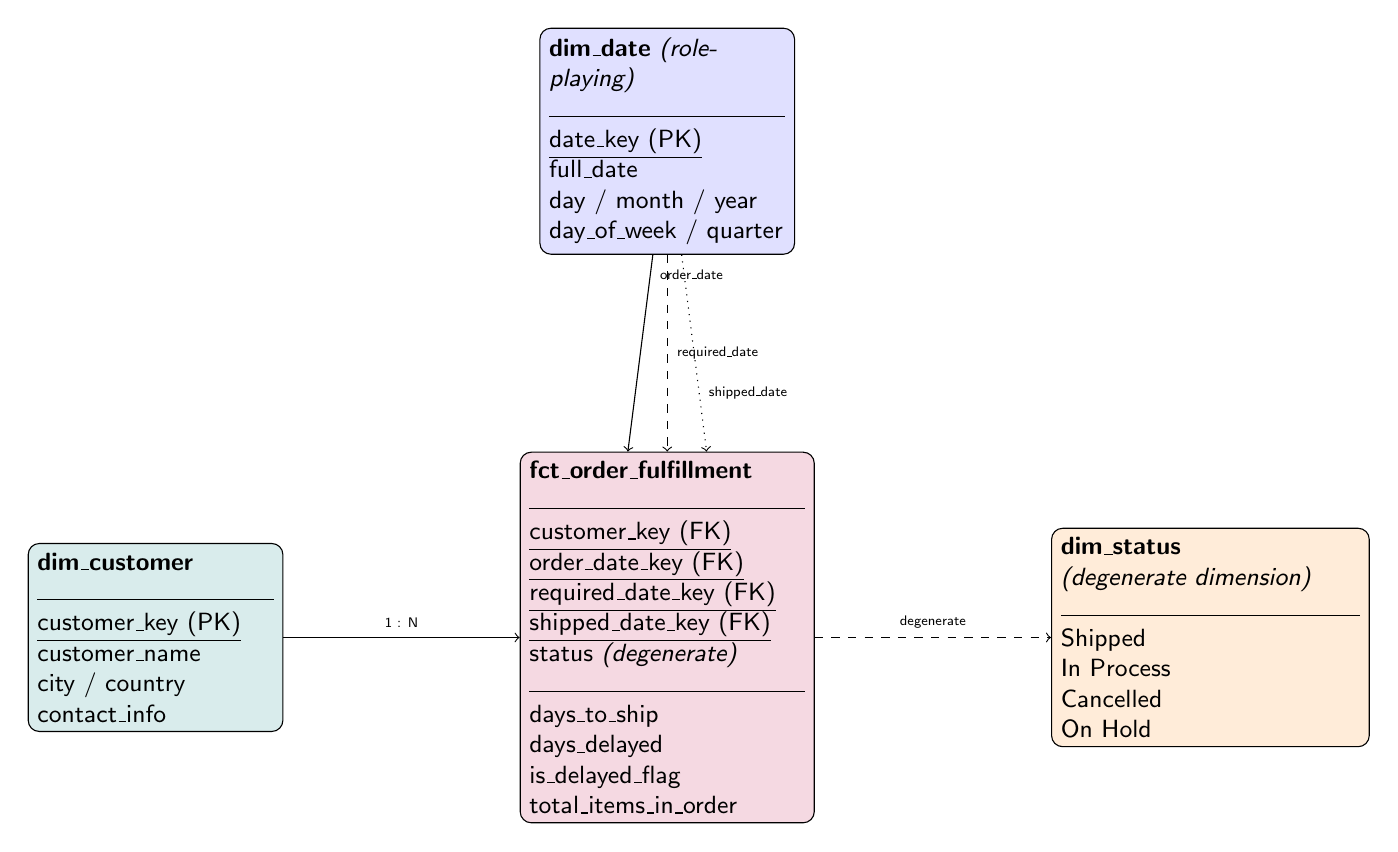
\begin{tikzpicture}[
        node distance=1cm,
        fact/.style={rectangle, draw, fill=purple!15, text width=3.5cm, align=left, rounded corners, font=\small},
        dim/.style={rectangle, draw, fill=teal!15, text width=3cm, align=left, rounded corners, font=\small},
        dimdate/.style={rectangle, draw, fill=blue!12, text width=3cm, align=left, rounded corners, font=\small},
        dimstatus/.style={rectangle, draw, fill=orange!15, text width=3.8cm, align=left, rounded corners, font=\small},
    ]

    %% Fact Table (center)
    \node[fact] (fact) {
        \textbf{fct\_order\_fulfillment} \\
        \rule{\linewidth}{0.4pt} \\
        \underline{customer\_key (FK)} \\
        \underline{order\_date\_key (FK)} \\
        \underline{required\_date\_key (FK)} \\
        \underline{shipped\_date\_key (FK)} \\
        status \textit{(degenerate)} \\
        \rule{\linewidth}{0.4pt} \\
        days\_to\_ship \\
        days\_delayed \\
        is\_delayed\_flag \\
        total\_items\_in\_order
    };

    %% dim_customer (left)
    \node[dim, left=3cm of fact] (dimcust) {
        \textbf{dim\_customer} \\
        \rule{\linewidth}{0.4pt} \\
        \underline{customer\_key (PK)} \\
        customer\_name \\
        city / country \\
        contact\_info
    };

    %% dim_date (top) — shared, role-playing 3×
    \node[dimdate, above=2.5cm of fact] (dimdate) {
        \textbf{dim\_date} \textit{(role-playing)} \\
        \rule{\linewidth}{0.4pt} \\
        \underline{date\_key (PK)} \\
        full\_date \\
        day / month / year \\
        day\_of\_week / quarter
    };

    %% dim_status (right) — degenerate
    \node[dimstatus, right=3cm of fact] (dimstat) {
        \textbf{dim\_status} \\
        \textit{(degenerate dimension)} \\
        \rule{\linewidth}{0.4pt} \\
        Shipped \\
        In Process \\
        Cancelled \\
        On Hold
    };

    %% Arrows
    \draw[->] (dimcust) -- node[above, font=\tiny]{1 : N} (fact);
    \draw[->] (dimdate) -- node[pos=0.1, right, font=\tiny]{order\_date}
              ([xshift=-0.5cm]fact.north);
    \draw[->, dashed] (dimdate) -- node[pos=0.5, right, font=\tiny]{required\_date}
              (fact.north);
    \draw[->, dotted] (dimdate) -- node[pos=0.7, right, font=\tiny]{shipped\_date}
              ([xshift=0.5cm]fact.north);
    \draw[->, dashed] (fact) -- node[above, font=\tiny]{degenerate} (dimstat);

    \end{tikzpicture}%
    }
    \caption{Star Schema --- \texttt{fct\_order\_fulfillment} (Accumulating Snapshot)}
    \label{fig:star-schema-fulfillment}
\end{figure}

\subsection{Implementasi dbt (Data Transformation)}
Langkah ini melibatkan pembuatan model SQL di dbt untuk mentransformasi data \textit{staging} menjadi tabel fakta operasional.

\begin{lstlisting}[language=Python, caption=Skrip Python untuk Menyiapkan Model dbt Fulfillment]
def setup_dbt_content():
    # Menyiapkan direktori proyek
    folders = ["models/staging", "models/dimensions", "models/marts"]
    for folder in folders:
        os.makedirs(os.path.join(PROJECT_BASE, folder), exist_ok=True)

    # Implementasi Logika SQL Marts
    mart_files_4 = {
      "models/dimensions/dim_status.sql": """
          select distinct status as order_status
          from {{ ref('stg_orders') }}
      """,

      "models/marts/fct_order_fulfillment.sql": """
          with orders as (
              select * from {{ ref('stg_orders') }}
          ),
          order_items_summary as (
              select
                  order_id,
                  count(product_code) as total_items_in_order
              from {{ ref('stg_orderdetails') }}
              group by 1
          )

          select
              o.order_id as order_key,
              o.customer_id,
              o.order_date,
              o.required_date,
              o.shipped_date,
              o.status as order_status,

              -- Kalkulasi Logistik
              date_diff('day', o.order_date, o.shipped_date) as days_to_ship,
              date_diff('day', o.required_date, o.shipped_date) as days_delayed,

              case
                  when o.shipped_date > o.required_date then 1
                  else 0
              end as is_delayed_flag,

              s.total_items_in_order

          from orders o
          left join order_items_summary s on o.order_id = s.order_id
      """
    }

    # Penulisan file ke sistem
    for rel_path, content in mart_files_4.items():
        full_path = os.path.join(PROJECT_BASE, rel_path)
        with open(full_path, "w") as f:
            f.write(content.strip())

    print("[OK] data marts siap!")
\end{lstlisting}

\subsection{Output Verifikasi}
Setelah menjalankan fungsi di atas, sistem akan memberikan konfirmasi sebagai berikut:
\begin{verbatim}
[INFO] Menyiapkan model di: /content/drive/MyDrive/Tugas DBT/dbt_classicmodels
[OK] data marts siap!
\end{verbatim}

\subsection{Nilai Strategis Bisnis}
Berbeda dengan model pendapatan (Revenue) yang fokus pada hasil finansial, model ini fokus pada \textbf{Operational Excellence}. Jika performa logistik buruk (banyak pesanan terlambat), maka tingkat kepuasan pelanggan akan menurun, yang pada akhirnya akan mengancam \textit{future revenue}.

\subsubsection{Business Process 5: Inventory Valuation \& Product Health}
Menghitung modal yang tertanam di gudang dan mengidentifikasi risiko \textit{stock-out}.
Tabel status inventori memantau nilai modal yang tertahan di
gudang sekaligus mengidentifikasi risiko \textit{stock-out} dan
\textit{overstock} pada level produk. \textit{Grain}: 1 produk (snapshot
stok saat ini). Berbeda dengan fact table transaksional, model ini bersifat
\textit{point-in-time snapshot} sehingga setiap eksekusi mencerminkan kondisi
gudang pada saat pipeline dijalankan.
 
Analisis dilakukan melalui tiga kueri terpisah yang masing-masing menjawab
pertanyaan bisnis berbeda: valuasi modal per lini produk, deteksi
\textit{dead stock}, dan deteksi risiko \textit{stock-out}.
 
%% --- Query 1 ---
\paragraph{Kueri 1 — Total Inventory Value by Product Line.}
Menghitung berapa besar modal yang tertahan di gudang per kategori produk,
diperoleh dari perkalian \texttt{quantityInStock} dengan \texttt{buyPrice}
untuk setiap produk, lalu diagregasi per \texttt{productLine}.
 
\begin{lstlisting}[
  language=SQL,
  caption={Valuasi stok per lini produk},
  label={lst:inv-value-detail},
  basicstyle=\ttfamily\footnotesize,
  keywordstyle=\color{blue!70!black}\bfseries,
  commentstyle=\color{gray}\itshape,
  showstringspaces=false,
  breaklines=true,
  frame=single,
  numbers=left,
  numberstyle=\tiny\color{gray},
  numbersep=8pt,
  xleftmargin=15pt
]
SELECT
    p.productLine                            AS product_line,
    SUM(p.quantityInStock)                   AS total_items_in_stock,
    SUM(p.quantityInStock * p.buyPrice)      AS total_inventory_value
FROM products p
GROUP BY p.productLine
ORDER BY total_inventory_value DESC;
\end{lstlisting}
 
\texttt{total\_inventory\_value} menjadi KPI utama manajemen modal kerja.
Lini produk dengan nilai tertinggi menjadi prioritas evaluasi efisiensi
rotasi stok.
 
%% --- Query 2 ---
\paragraph{Kueri 2 — Top 5 Dead Stock / Overstocked Products.}
Mengidentifikasi produk dengan stok sangat banyak tetapi historis
penjualannya rendah. Metrik kunci adalah
\texttt{stock\_to\_sales\_ratio} = \texttt{current\_stock} $\div$
\texttt{total\_sold}; rasio tinggi mengindikasikan modal idle yang berisiko.
 
\begin{lstlisting}[
  language=SQL,
  caption={Deteksi produk \textit{dead stock} (rasio stok-ke-penjualan tertinggi)},
  label={lst:inv-overstock-detail},
  basicstyle=\ttfamily\footnotesize,
  keywordstyle=\color{blue!70!black}\bfseries,
  commentstyle=\color{gray}\itshape,
  showstringspaces=false,
  breaklines=true,
  frame=single,
  numbers=left,
  numberstyle=\tiny\color{gray},
  numbersep=8pt,
  xleftmargin=15pt
]
WITH sales_history AS (
    SELECT productCode,
           SUM(quantityOrdered) AS total_sold
    FROM orderdetails
    GROUP BY productCode
)
SELECT
    p.productCode                                AS product_code,
    p.productName                                AS product_name,
    p.quantityInStock                            AS current_stock,
    COALESCE(s.total_sold, 0)                    AS total_sold,
    ROUND(p.quantityInStock * 1.0
          / NULLIF(s.total_sold, 0), 2)          AS stock_to_sales_ratio
FROM products p
LEFT JOIN sales_history s ON p.productCode = s.productCode
WHERE p.quantityInStock > 1000   -- filter minimum relevansi
ORDER BY stock_to_sales_ratio DESC NULLS FIRST
LIMIT 5;
\end{lstlisting}
 
\texttt{NULLIF(s.total\_sold, 0)} mencegah pembagian dengan nol untuk produk
yang belum pernah terjual sama sekali, yang kemudian ditangkap oleh
\texttt{NULLS FIRST} agar muncul di posisi teratas sebagai prioritas
penanganan.
 
%% --- Query 3 ---
\paragraph{Kueri 3 — Top 5 Stock-Out Risk Products.}
Mengidentifikasi produk yang sangat laku namun sisa stoknya sudah
sangat sedikit. Filter \texttt{quantityInStock < 500} menetapkan ambang
peringatan, sedangkan pengurutan \texttt{stock\_to\_sales\_ratio ASC}
menempatkan produk dengan risiko tertinggi di posisi pertama.
 
\begin{lstlisting}[
  language=SQL,
  caption={Deteksi risiko \textit{stock-out} (rasio stok-ke-penjualan terendah)},
  label={lst:inv-stockout-detail},
  basicstyle=\ttfamily\footnotesize,
  keywordstyle=\color{blue!70!black}\bfseries,
  commentstyle=\color{gray}\itshape,
  showstringspaces=false,
  breaklines=true,
  frame=single,
  numbers=left,
  numberstyle=\tiny\color{gray},
  numbersep=8pt,
  xleftmargin=15pt
]
WITH sales_history AS (
    SELECT productCode,
           SUM(quantityOrdered) AS total_sold
    FROM orderdetails
    GROUP BY productCode
)
SELECT
    p.productCode                                AS product_code,
    p.productName                                AS product_name,
    p.quantityInStock                            AS current_stock,
    s.total_sold,
    ROUND(p.quantityInStock * 1.0
          / NULLIF(s.total_sold, 0), 2)          AS stock_to_sales_ratio
FROM products p
JOIN sales_history s ON p.productCode = s.productCode
WHERE p.quantityInStock < 500    -- ambang peringatan stock-out
ORDER BY stock_to_sales_ratio ASC
LIMIT 5;
\end{lstlisting}
 
Perbedaan antara Kueri~2 dan Kueri~3 terletak pada jenis \texttt{JOIN}:
Kueri~2 menggunakan \texttt{LEFT JOIN} untuk menangkap produk tanpa riwayat
penjualan sama sekali, sedangkan Kueri~3 menggunakan \texttt{INNER JOIN}
karena produk tanpa penjualan tidak dapat memiliki risiko \textit{stock-out}
yang bermakna.
 
Ketiga kueri ini secara bersama-sama membentuk laporan \textit{Product Health
Dashboard} yang memungkinkan tim operasional mengambil keputusan: negosiasi
ulang harga atau promosi untuk produk \textit{overstocked}, serta percepatan
pemesanan ulang untuk produk berisiko \textit{stock-out}.
 Tabel status inventori memantau nilai modal yang tertahan di
gudang sekaligus mengidentifikasi risiko \textit{stock-out} dan
\textit{overstock} pada level produk. \textit{Grain}: 1 produk (snapshot
stok saat ini). Berbeda dengan fact table transaksional, model ini bersifat
\textit{point-in-time snapshot} sehingga setiap eksekusi mencerminkan kondisi
gudang pada saat pipeline dijalankan.
 
Analisis dilakukan melalui tiga kueri terpisah yang masing-masing menjawab
pertanyaan bisnis berbeda: valuasi modal per lini produk, deteksi
\textit{dead stock}, dan deteksi risiko \textit{stock-out}.
 
%% --- Query 1 ---
\paragraph{Kueri 1 — Total Inventory Value by Product Line.}
Menghitung berapa besar modal yang tertahan di gudang per kategori produk,
diperoleh dari perkalian \texttt{quantityInStock} dengan \texttt{buyPrice}
untuk setiap produk, lalu diagregasi per \texttt{productLine}.
 
\begin{lstlisting}[
  language=SQL,
  caption={Valuasi stok per lini produk},
  label={lst:inv-value},
  basicstyle=\ttfamily\footnotesize,
  keywordstyle=\color{blue!70!black}\bfseries,
  commentstyle=\color{gray}\itshape,
  showstringspaces=false,
  breaklines=true,
  frame=single,
  numbers=left,
  numberstyle=\tiny\color{gray},
  numbersep=8pt,
  xleftmargin=15pt
]
SELECT
    p.productLine                            AS product_line,
    SUM(p.quantityInStock)                   AS total_items_in_stock,
    SUM(p.quantityInStock * p.buyPrice)      AS total_inventory_value
FROM products p
GROUP BY p.productLine
ORDER BY total_inventory_value DESC;
\end{lstlisting}
 
\texttt{total\_inventory\_value} menjadi KPI utama manajemen modal kerja.
Lini produk dengan nilai tertinggi menjadi prioritas evaluasi efisiensi
rotasi stok.
 
%% --- Query 2 ---
\paragraph{Kueri 2 — Top 5 Dead Stock / Overstocked Products.}
Mengidentifikasi produk dengan stok sangat banyak tetapi historis
penjualannya rendah. Metrik kunci adalah
\texttt{stock\_to\_sales\_ratio} = \texttt{current\_stock} $\div$
\texttt{total\_sold}; rasio tinggi mengindikasikan modal idle yang berisiko.
 
\begin{lstlisting}[
  language=SQL,
  caption={Deteksi produk \textit{dead stock} (rasio stok-ke-penjualan tertinggi)},
  label={lst:inv-overstock},
  basicstyle=\ttfamily\footnotesize,
  keywordstyle=\color{blue!70!black}\bfseries,
  commentstyle=\color{gray}\itshape,
  showstringspaces=false,
  breaklines=true,
  frame=single,
  numbers=left,
  numberstyle=\tiny\color{gray},
  numbersep=8pt,
  xleftmargin=15pt
]
WITH sales_history AS (
    SELECT productCode,
           SUM(quantityOrdered) AS total_sold
    FROM orderdetails
    GROUP BY productCode
)
SELECT
    p.productCode                                AS product_code,
    p.productName                                AS product_name,
    p.quantityInStock                            AS current_stock,
    COALESCE(s.total_sold, 0)                    AS total_sold,
    ROUND(p.quantityInStock * 1.0
          / NULLIF(s.total_sold, 0), 2)          AS stock_to_sales_ratio
FROM products p
LEFT JOIN sales_history s ON p.productCode = s.productCode
WHERE p.quantityInStock > 1000   -- filter minimum relevansi
ORDER BY stock_to_sales_ratio DESC NULLS FIRST
LIMIT 5;
\end{lstlisting}
 
\texttt{NULLIF(s.total\_sold, 0)} mencegah pembagian dengan nol untuk produk
yang belum pernah terjual sama sekali, yang kemudian ditangkap oleh
\texttt{NULLS FIRST} agar muncul di posisi teratas sebagai prioritas
penanganan.
 
%% --- Query 3 ---
\paragraph{Kueri 3 — Top 5 Stock-Out Risk Products.}
Mengidentifikasi produk yang sangat laku namun sisa stoknya sudah
sangat sedikit. Filter \texttt{quantityInStock < 500} menetapkan ambang
peringatan, sedangkan pengurutan \texttt{stock\_to\_sales\_ratio ASC}
menempatkan produk dengan risiko tertinggi di posisi pertama.
 
\begin{lstlisting}[
  language=SQL,
  caption={Deteksi risiko \textit{stock-out} (rasio stok-ke-penjualan terendah)},
  label={lst:inv-stockout},
  basicstyle=\ttfamily\footnotesize,
  keywordstyle=\color{blue!70!black}\bfseries,
  commentstyle=\color{gray}\itshape,
  showstringspaces=false,
  breaklines=true,
  frame=single,
  numbers=left,
  numberstyle=\tiny\color{gray},
  numbersep=8pt,
  xleftmargin=15pt
]
WITH sales_history AS (
    SELECT productCode,
           SUM(quantityOrdered) AS total_sold
    FROM orderdetails
    GROUP BY productCode
)
SELECT
    p.productCode                                AS product_code,
    p.productName                                AS product_name,
    p.quantityInStock                            AS current_stock,
    s.total_sold,
    ROUND(p.quantityInStock * 1.0
          / NULLIF(s.total_sold, 0), 2)          AS stock_to_sales_ratio
FROM products p
JOIN sales_history s ON p.productCode = s.productCode
WHERE p.quantityInStock < 500    -- ambang peringatan stock-out
ORDER BY stock_to_sales_ratio ASC
LIMIT 5;
\end{lstlisting}
 
Perbedaan antara Kueri~2 dan Kueri~3 terletak pada jenis \texttt{JOIN}:
Kueri~2 menggunakan \texttt{LEFT JOIN} untuk menangkap produk tanpa riwayat
penjualan sama sekali, sedangkan Kueri~3 menggunakan \texttt{INNER JOIN}
karena produk tanpa penjualan tidak dapat memiliki risiko \textit{stock-out}
yang bermakna.
 
Ketiga kueri ini secara bersama-sama membentuk laporan \textit{Product Health
Dashboard} yang memungkinkan tim operasional mengambil keputusan: negosiasi
ulang harga atau promosi untuk produk \textit{overstocked}, serta percepatan
pemesanan ulang untuk produk berisiko \textit{stock-out}.
 


\begin{itemize}
    \item \textbf{Stock-to-Sales Ratio:} \texttt{qty\_stock / total\_units\_sold}.
\end{itemize}

\section{Part 4: Data Exploration and Deployment}

\subsection{Data Exploration}

Pada tahap ini, kita mengeksplorasi insight bisnis dari tabel-tabel yang telah dibangun menggunakan query SQL melalui koneksi \texttt{DuckDB} di dalam Python.

\subsubsection{Kode Implementasi}

\begin{lstlisting}[language=Python, caption={Step 8 -- Explore Business Insight}, label={lst:step8}]
import duckdb
import pandas as pd

insight_query = """
    SELECT
        p.product_line,
        ROUND(SUM(f.quantity_ordered * f.price_each), 2)
            AS total_revenue,
        ROUND(SUM(f.quantity_ordered * (f.price_each - p.buy_price)), 2)
            AS total_profit,
        ROUND(
            (SUM(f.quantity_ordered * (f.price_each - p.buy_price))
             / SUM(f.quantity_ordered * f.price_each)) * 100, 2
        ) AS margin_pct
    FROM fct_order_lines f
    JOIN stg_products p ON f.product_code = p.product_code
    GROUP BY 1
    ORDER BY total_revenue DESC
"""

def run_insight_table(query):
    conn = duckdb.connect(database_path)
    try:
        print("Menghasilkan Tabel Insight Bisnis...")
        df = conn.execute(query).df()
        if df.empty:
            print("Tidak ada data. Pastikan tabel sudah terisi.")
        else:
            pd.options.display.float_format = '{:,.2f}'.format
            display(df)
    except Exception as e:
        print(f"Error pada Query: {e}")
    finally:
        conn.close()

run_insight_table(insight_query)
\end{lstlisting}

\subsubsection{Penjelasan Query SQL}

Query di atas melakukan agregasi dari dua tabel utama:

\begin{itemize}
    \item Tabel fakta pesanan menyimpan detail setiap baris pesanan, termasuk jumlah pesanan dan harga jual.
    \item Tabel staging produk menyimpan harga beli/HPP dan lini produk.
\end{itemize}

Ketiga metrik yang dihitung adalah:

\begin{enumerate}
    \item \textbf{\texttt{total\_revenue}} — total pendapatan kotor per lini produk, dihitung sebagai $\sum (\texttt{quantity\_ordered} \times \texttt{price\_each})$.
    \item \textbf{\texttt{total\_profit}} — total laba bersih per lini produk, dihitung sebagai $\sum (\texttt{quantity\_ordered} \times (\texttt{price\_each} - \texttt{buy\_price}))$.
    \item \textbf{\texttt{margin\_pct}} — persentase margin keuntungan, dihitung sebagai $\frac{\texttt{total\_profit}}{\texttt{total\_revenue}} \times 100$.
\end{enumerate}

\subsubsection{Hasil Output}

Tabel~\ref{tab:insight-revenue} menampilkan hasil query yang menunjukkan perbandingan \textit{revenue}, \textit{profit}, dan \textit{margin} antar lini produk, diurutkan dari pendapatan tertinggi.

\begin{table}[H]
    \centering
    \caption{Revenue by Product Line with Margin}
    \label{tab:insight-revenue}
    \small
    \begin{tabular}{lrrr}
        \toprule
        \textbf{Product Line} & \textbf{Total Revenue} & \textbf{Total Profit} & \textbf{Margin (\%)} \\
        \midrule
        Classic Cars      & 3,853,922.49 & 1,526,212.20 & 39.60 \\
        Vintage Cars      & 1,797,559.63 &   737,268.33 & 41.01 \\
        Motorcycles       & 1,121,426.12 &   469,255.30 & 41.84 \\
        Trucks and Buses  & 1,024,113.57 &   400,553.22 & 39.11 \\
        Planes            &   954,637.54 &   365,960.71 & 38.34 \\
        Ships             &   663,998.34 &   261,289.47 & 39.35 \\
        Trains            &   188,532.92 &    65,341.02 & 34.66 \\
        \bottomrule
    \end{tabular}
\end{table}

\textbf{Insight utama:} \textit{Classic Cars} mendominasi total revenue dengan nilai \$3,853,922.49, sementara \textit{Motorcycles} mencatatkan margin tertinggi sebesar 41.84\%. Lini \textit{Trains} memiliki kontribusi revenue terkecil sekaligus margin paling rendah (34.66\%).

% ─────────────────────────────────────────────
\subsection{Deployment}

Tahap ini membangkitkan dokumentasi otomatis dari proyek dbt, termasuk \textit{lineage graph} yang memvisualisasikan aliran data dari \textit{staging table} hingga \textit{fact table}.

\subsubsection{Kode Implementasi}

\begin{lstlisting}[language=bash, caption={Step 9 -- Generate dan Serve dbt Docs}, label={lst:step9}]
# Generate catalog.json dan dokumentasi
!dbt docs generate

# Forward port 8088 agar dapat diakses dari browser
from google.colab import output
output.serve_kernel_port_as_window(8088)

# Jalankan server dokumentasi
!dbt docs serve --port 8088
\end{lstlisting}

\subsubsection{Penjelasan Perintah}

\begin{itemize}
    \item \texttt{dbt docs generate} — memindai seluruh model, sumber data, dan metadata proyek, lalu menghasilkan file \texttt{catalog.json} di direktori \texttt{target/}. File ini berisi informasi skema, tipe data kolom, dan deskripsi tiap model.
    \item \texttt{output.serve\_kernel\_port\_as\_window(8088)} — fungsi dari Google Colab untuk meneruskan (\textit{forward}) port kernel ke jendela browser, sehingga server lokal dapat diakses dari luar lingkungan Colab.
    \item \texttt{dbt docs serve --port 8088} — menjalankan server web statis pada port 8088 yang menyajikan dokumentasi interaktif beserta \textit{lineage graph}.
\end{itemize}

\subsubsection{Output dan Log Eksekusi}

Setelah perintah dijalankan, terminal menampilkan log berikut:

\begin{lstlisting}[language=bash, caption={Log eksekusi dbt docs generate \& serve}]
Running with dbt=1.11.9
Registered adapter: duckdb=1.10.1
Found 18 models, 4 data tests, 8 sources, 477 macros
Concurrency: 4 threads (target='dev')
Building catalog
Catalog written to .../target/catalog.json
Running with dbt=1.11.9
Serving docs at 8088
To access from your browser, navigate to: http://localhost:8088
\end{lstlisting}

Dokumentasi dapat diakses melalui \texttt{http://localhost:8088}. Pada antarmuka tersebut tersedia \textit{lineage graph} interaktif yang menampilkan ketergantungan antar model secara visual, dari lapisan \textit{staging} (\texttt{stg\_*}) hingga lapisan \textit{dimension} (\texttt{dim\_*}) dan \textit{fact} (\texttt{fct\_*}).

\begin{figure}[H]
    \centering
    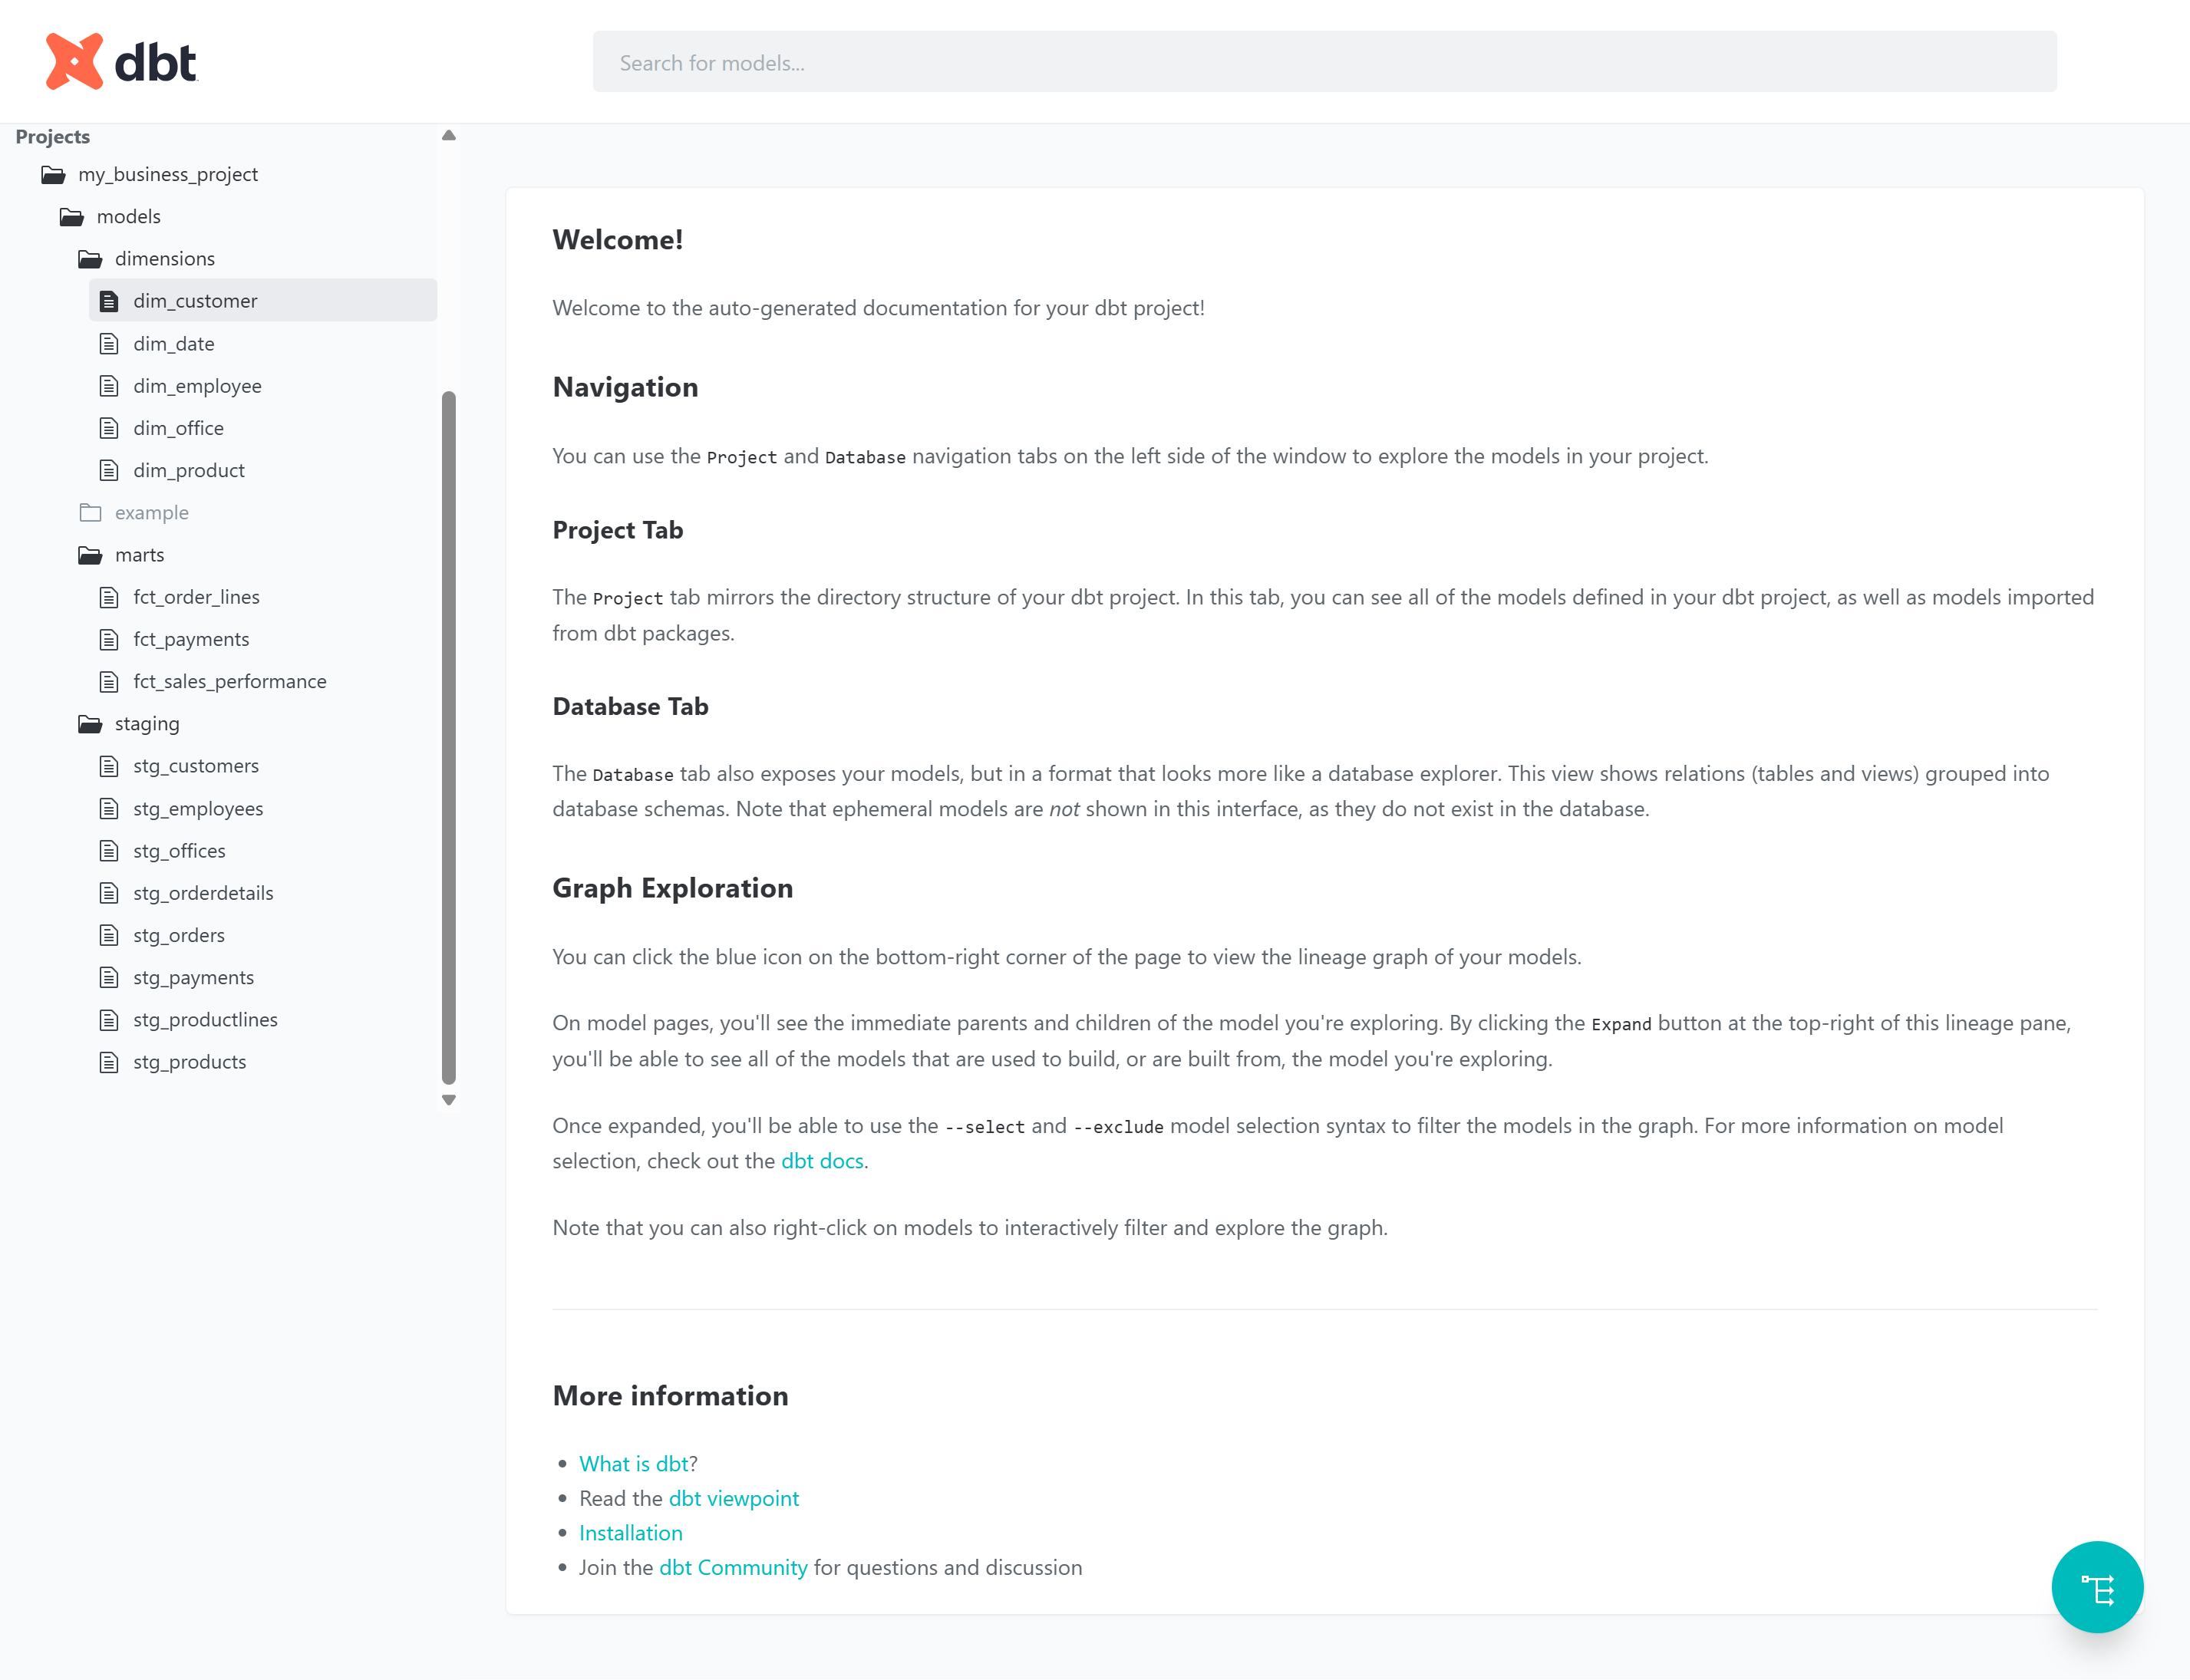
\includegraphics[width=0.95\textwidth]{figures/home-dbt.png}
    \caption{Dokumentasi yang diakses lewat localhost}
    \label{fig:home-dbt}
\end{figure}

\begin{figure}[H]
    \centering
    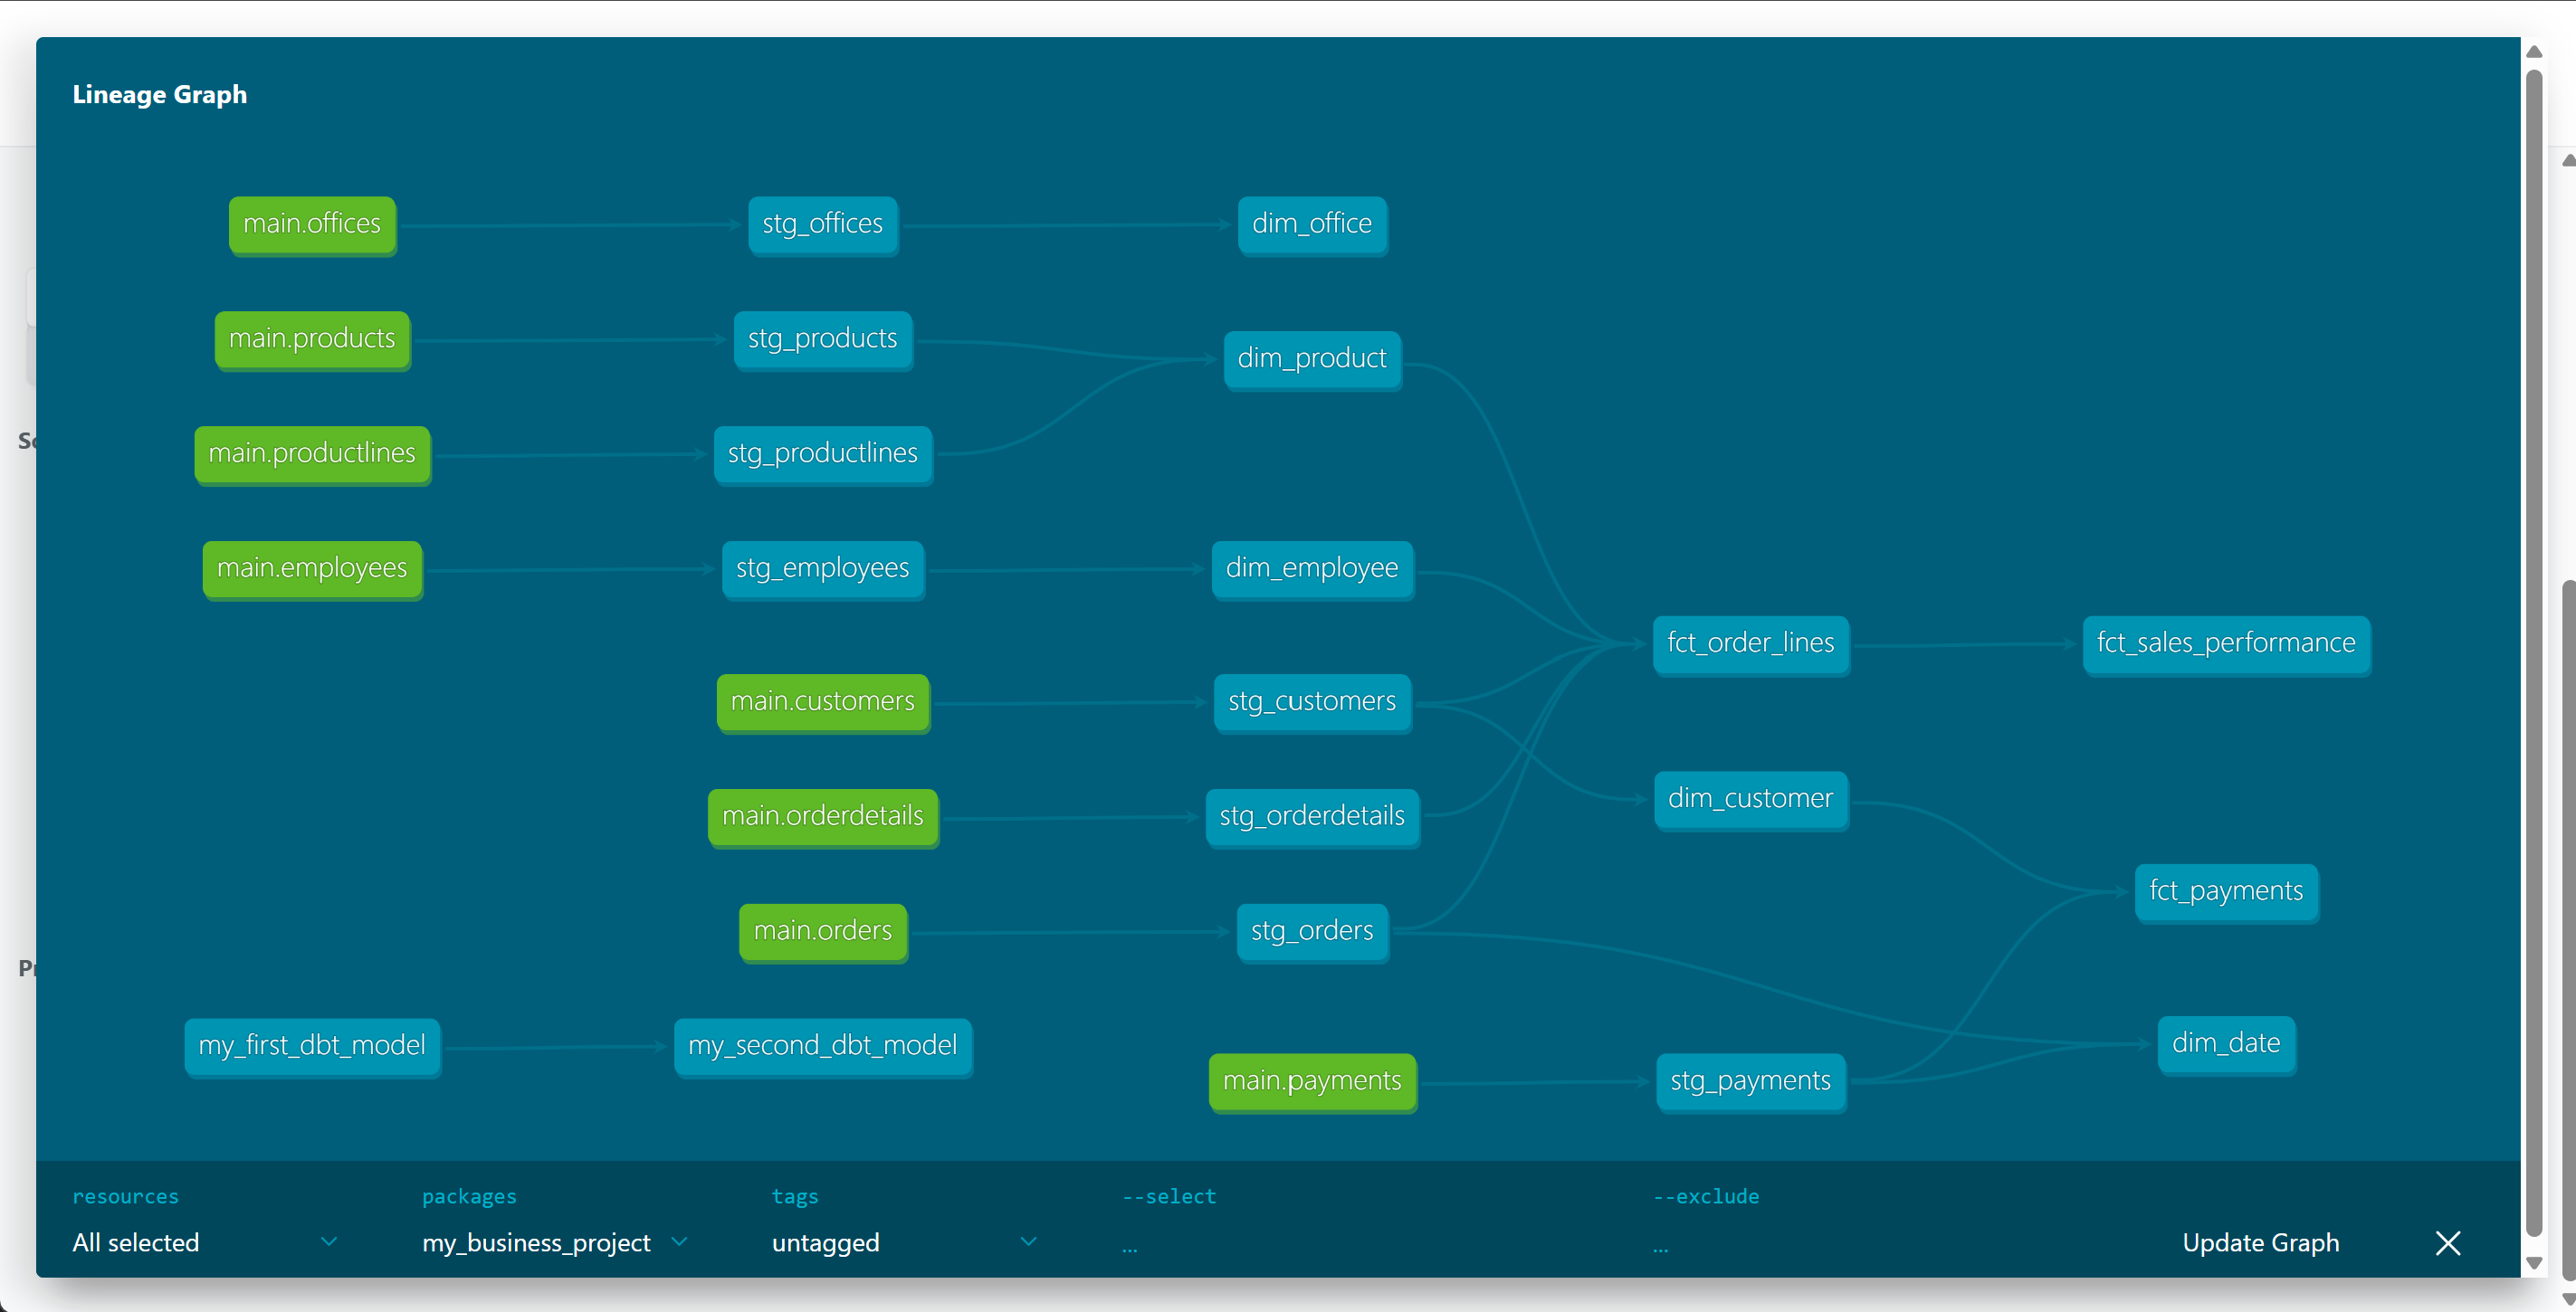
\includegraphics[width=0.95\textwidth]{figures/graph-dbt.png}
    \caption{Lineage Graph Interaktif yang menampilkan relasi antar lapisan staging, dimension dan fact}
    \label{fig:graph-dbt}
\end{figure}

\subsection{Analisis Lineage Graph (Silsilah Data)}

Berdasarkan grafik tersebut, alur data dibagi menjadi tiga tingkatan utama sesuai dengan prinsip \textit{Medallion Architecture}:

\begin{enumerate}
    \item \textbf{Source Layer (Main):} Titik awal data yang berasal dari database DuckDB (\texttt{main}). Terdapat empat tabel sumber utama yang diidentifikasi, yaitu \texttt{customers}, \texttt{orderdetails}, \texttt{orders}, dan \texttt{products}.
    \item \textbf{Staging Layer (Silver):} Data mentah ditransformasikan menjadi model \textit{staging} (\texttt{stg\_}). 
    \begin{itemize}
        \item \texttt{stg\_customers}, \texttt{stg\_orderdetails}, \texttt{stg\_orders}, dan \texttt{stg\_products} melakukan pembersihan awal (seperti penggantian nama kolom atau perubahan tipe data).
    \end{itemize}
    \item \textbf{Intermediate/Dimension Layer:} 
    \begin{itemize}
        \item \texttt{dim\_customer} mengambil referensi langsung dari \texttt{stg\_customers}.
        \item \texttt{dim\_product} mengambil referensi dari \texttt{stg\_products}.
    \end{itemize}
    \item \textbf{Mart/Fact Layer (Gold):} Puncak dari transformasi adalah tabel \texttt{fct\_order\_lines}. Tabel fakta ini memiliki ketergantungan (\textit{dependencies}) paling kompleks karena menggabungkan data dari \texttt{stg\_orderdetails}, \texttt{stg\_orders}, serta melakukan \textit{lookup} ke tabel dimensi \texttt{dim\_customer} dan \texttt{dim\_product}.
\end{enumerate}

\subsubsection{Fungsi dan Manfaat Lineage Graph}
\begin{itemize}
    \item \textbf{Data Traceability:} Memungkinkan pengembang untuk melacak asal-usul setiap kolom data. Jika ditemukan kesalahan pada \texttt{fct\_order\_lines}, pengembang dapat dengan mudah menelusuri ke belakang apakah kesalahan terjadi di level \textit{staging} atau pada data sumber.
    \item \textbf{Impact Analysis:} Sebelum melakukan perubahan pada tabel di level \textit{staging}, tim data dapat melihat model mana saja yang akan terdampak (misalnya, mengubah \texttt{stg\_products} akan berdampak pada \texttt{dim\_product} dan \texttt{fct\_order\_lines}).
    \item \textbf{Optimasi Kueri:} dbt menggunakan grafik ini untuk menentukan urutan eksekusi yang paling optimal
\end{itemize}
\clearpage
\subsection{Rincian Kontribusi Kelompok}
Seluruh tahapan dalam studi kasus ini dikerjakan secara kolaboratif dengan pembagian tanggung jawab yang mencakup penyusunan konten modul, penyiapan lingkungan teknis, hingga eksekusi transformasi data. Berikut adalah matriks kontribusi anggota kelompok yang merujuk pada struktur pembahasan dalam laporan ini:
\begin{table}[ht]
\centering
\caption{Rincian Kontribusi Anggota Kelompok Berdasarkan Struktur Laporan}
\label{tab:kontribusi-kelompok-detail}
\begin{tabular}{|c|l|p{8.5cm}|}
\hline
\textbf{No} & \textbf{Nama Anggota} & \textbf{Kontribusi Berdasarkan Struktur Bab} \\ \hline
1 & Engelbertus Rande & \textbf{Bab I (dbt Sebagai Tools Bantu):} Menyusun pengenalan dbt, konsep arsitektur, struktur model, serta dokumentasi standar \textit{Data Quality}. \\ \hline
2 & Gilbert Fandiliam Mooy & \textbf{Bab II (Penyiapan Lingkungan dbt):} Menyusun perbandingan dbt Core vs Cloud, dokumentasi instalasi \textit{package}, serta workflow inisialisasi proyek. \\ \hline
3 & Sinta Siti Nuriah & \textbf{Bab III (Studi Kasus - Fase Awal):} Menyusun skema DB/DW, konversi MySQL ke DuckDB, penyiapan \textit{Staging Layer}, serta implementasi \textit{Initial Code} dbt. \\ \hline
4 & Vicky Mahfudy & \textbf{Bab III (Studi Kasus - Fase Akhir):} Implementasi \textit{Dimensional Modeling} (Fakta \& Dimensi), optimasi \textit{Star Schema}, \textit{Data Exploration}, serta validasi kesesuaian antara modul dan teknis. \\ \hline
\end{tabular}
\end{table}

\part{Synthetic Data Generation}
\chapter{Synthetic Data Generation}

% ============================================================
%  BAB IV: SYNTHETIC DATA GENERATION
% ============================================================

 
\section{Strategi Generator Data Sintetik}
 
Proses perancangan ekosistem data rumah sakit dalam skala volume 12.000 transaksi mensyaratkan strategi simulasi logis yang merepresentasikan probabilitas keadaan lapangan yang sesungguhnya (\textit{Constraint Enforcement}). Metodologi augmentasi Python berlandaskan aturan berikut:
 
\begin{itemize}
    \item \textbf{Sinergi Kredensial Tarif Medis:} Beban tarif pada \texttt{biaya\_konsultasi} bukanlah angka yang diacak sepenuhnya, melainkan dikunci berdasarkan nilai kamus tarif spesialisasi.
    \item \textbf{Isolasi Logika Fasilitas Non-Inap:} Jika alokasi unit merujuk ke ``IGD'' atau ``Rawat Jalan'', algoritma menginstruksikan kalkulasi durasi inap absolut di angka 0 dan tidak membebankan biaya sewa ruangan.
    \item \textbf{Pembobotan Pemulihan Pasien Inap:} Pasien yang dialokasikan ke ``Rawat Inap'' memiliki hari rawat yang disimulasikan (1--14 hari) dan luaran klinis yang ditentukan oleh probabilitas empiris: 80\% dinyatakan Sembuh, dan hanya sisanya Dirujuk/Meninggal.
    \item \textbf{Logika Integritas Keuangan (\textit{Billing}):} \texttt{total\_biaya} dieksekusi secara matematis ketat melalui penjumlahan komponen linier: jasa dokter + obat farmasi + tindakan alat + sewa ruangan, meniadakan kesalahan agregasi fiskal pada Data Warehouse.
\end{itemize}
 
\section{Kode Generator Utama}
 
Berikut adalah \textit{source code} Python yang dikompilasi secara deterministik untuk merakit data sumber transaksi rumah sakit operasional ke dalam direktori file CSV:
 
\begin{lstlisting}[language=Python, caption=Generator Data Sintetik Operasional Rumah Sakit]
import os
import random
from datetime import datetime, timedelta
import pandas as pd
from faker import Faker
 
# Inisialisasi Faker dengan lokalisasi Indonesia
fake = Faker('id_ID')
Faker.seed(42)
random.seed(42)
 
# Konfigurasi Jumlah Data
TOTAL_PASIEN = 2500
TOTAL_DOKTER = 80
TOTAL_TRANSAKSI_KUNJUNGAN = 12000
 
print("Memulai pembuatan dataset sintetik rumah sakit...")
 
# ==========================================
# 1. GENERATE TABEL SUMBER: PASIEN
# ==========================================
data_pasien = []
golongan_darah_opsi = ['A', 'B', 'AB', 'O']
jenis_kelamin_opsi = ['Laki-laki', 'Perempuan']
 
for pasien_id in range(1, TOTAL_PASIEN + 1):
    jk = random.choice(jenis_kelamin_opsi)
    nama = fake.name_male() if jk == 'Laki-laki' else fake.name_female()
    data_pasien.append({
        'id_pasien'      : f'PSN-{pasien_id:05d}',
        'nama_pasien'    : nama,
        'jenis_kelamin'  : jk,
        'tanggal_lahir'  : fake.date_of_birth(minimum_age=0, maximum_age=85)
                               .strftime('%Y-%m-%d'),
        'alamat'         : fake.street_address(),
        'kota'           : fake.city(),
        'golongan_darah' : random.choice(golongan_darah_opsi)
    })
df_pasien = pd.DataFrame(data_pasien)
 
# ==========================================
# 2. GENERATE TABEL SUMBER: DOKTER
# ==========================================
data_dokter = []
spesialisasi_opsi = {
    'Umum': 30, 'Anak': 40, 'Penyakit Dalam': 50,
    'Bedah': 60, 'Jantung': 80, 'Saraf': 70, 'Mata': 45
}
 
for dokter_id in range(1, TOTAL_DOKTER + 1):
    spesialisasi = random.choice(list(spesialisasi_opsi.keys()))
    biaya_konsultasi = spesialisasi_opsi[spesialisasi] * 1000
    data_dokter.append({
        'id_dokter'           : f'DKT-{dokter_id:03d}',
        'nama_dokter'         : fake.name(),
        'spesialisasi'        : spesialisasi,
        'biaya_konsultasi'    : biaya_konsultasi,
        'nomor_izin_praktek'  : f'STR-{random.randint(100000, 999999)}'
    })
df_dokter = pd.DataFrame(data_dokter)
 
# ==========================================
# 3. GENERATE TABEL SUMBER: KUNJUNGAN
# ==========================================
data_kunjungan = []
tipe_fasilitas_opsi   = ['IGD', 'Rawat Jalan', 'Rawat Inap']
status_keluar_opsi    = ['Sembuh', 'Dirujuk', 'Pulang Paksa', 'Meninggal']
metode_pembayaran_opsi = ['BPJS', 'Asuransi Swasta', 'Mandiri']
start_date = datetime(2025, 1, 1)
 
for kunjungan_id in range(1, TOTAL_TRANSAKSI_KUNJUNGAN + 1):
    pasien           = random.choice(data_pasien)
    dokter           = random.choice(data_dokter)
    tipe_fasilitas   = random.choice(tipe_fasilitas_opsi)
    metode_pembayaran = random.choice(metode_pembayaran_opsi)
 
    # Logika Lama Rawat Inap (Length of Stay)
    if tipe_fasilitas == 'Rawat Inap':
        lama_rawat    = random.randint(1, 14)
        status_keluar = random.choices(
            status_keluar_opsi, weights=[80, 12, 6, 2])[0]
        biaya_kamar   = lama_rawat * random.choice([250000, 500000, 1200000])
    else:
        lama_rawat    = 0
        status_keluar = 'Sembuh'
        biaya_kamar   = 0
 
    # Simulasi Komponen Biaya Medis
    biaya_konsul    = dokter['biaya_konsultasi']
    biaya_obat      = (random.randint(50000, 750000)
                       if tipe_fasilitas != 'IGD'
                       else random.randint(30000, 200000))
    biaya_tindakan  = (random.choice([0, 150000, 300000, 1500000])
                       if tipe_fasilitas in ['IGD', 'Rawat Inap'] else 0)
    total_biaya     = biaya_konsul + biaya_obat + biaya_tindakan + biaya_kamar
    tgl_kunjungan   = start_date + timedelta(days=random.randint(0, 450))
 
    data_kunjungan.append({
        'id_kunjungan'      : f'TX-{kunjungan_id:06d}',
        'id_pasien'         : pasien['id_pasien'],
        'id_dokter'         : dokter['id_dokter'],
        'tanggal_kunjungan' : tgl_kunjungan.strftime('%Y-%m-%d %H:%M:%S'),
        'tipe_fasilitas'    : tipe_fasilitas,
        'lama_rawat_hari'   : lama_rawat,
        'status_keluar'     : status_keluar,
        'metode_pembayaran' : metode_pembayaran,
        'biaya_konsultasi'  : biaya_konsul,
        'biaya_obat'        : biaya_obat,
        'biaya_tindakan'    : biaya_tindakan,
        'biaya_kamar'       : biaya_kamar,
        'total_biaya'       : total_biaya
    })
df_kunjungan = pd.DataFrame(data_kunjungan)
 
# ==========================================
# 4. MENYIMPAN DATA KE CSV
# ==========================================
OUTPUT_DIR = '/opt/airflow/data_generator/output'
os.makedirs(OUTPUT_DIR, exist_ok=True)
 
df_pasien.to_csv(os.path.join(OUTPUT_DIR, 'source_pasien.csv'), index=False)
df_dokter.to_csv(os.path.join(OUTPUT_DIR, 'source_dokter.csv'), index=False)
df_kunjungan.to_csv(os.path.join(OUTPUT_DIR, 'source_kunjungan.csv'), index=False)
 
print("Pembuatan dataset selesai!")
print(f"   - Total Pasien   : {len(df_pasien)} baris")
print(f"   - Total Dokter   : {len(df_dokter)} baris")
print(f"   - Total Kunjungan: {len(df_kunjungan)} baris")
\end{lstlisting}
 
\section{Contoh Data Mentah (Output source\_kunjungan.csv)}
 
Berikut adalah cuplikan simulasi hasil output transaksi yang memperlihatkan keutuhan integritas perhitungan \textit{billing} matematis dalam \textit{pipeline} DWBI ini.
 
\begin{table}[H]
\centering
\caption{Contoh Data Mentah Transaksi Kunjungan}
\small
\begin{tabularx}{\linewidth}{p{2cm}p{2cm}p{0.8cm}p{1.8cm}p{1.8cm}p{2cm}p{1.8cm}X}
\toprule
\textbf{ID Kunjungan} & \textbf{Fasilitas} & \textbf{LOS} & \textbf{Biaya Konsul} & \textbf{Biaya Obat} & \textbf{Biaya Tindakan} & \textbf{Biaya Kamar} & \textbf{Total (Rp)} \\
\midrule
TX-000001 & Rawat Inap   & 4 & 50.000  & 630.000 & 300.000   & 1.000.000 & 1.980.000 \\
TX-000002 & IGD          & 0 & 80.000  & 75.000  & 1.500.000 & 0         & 1.655.000 \\
TX-000003 & Rawat Jalan  & 0 & 30.000  & 125.000 & 0         & 0         & 155.000   \\
\bottomrule
\end{tabularx}
\end{table}
 
\section{Skema Sumber (Data Dictionary)}
 
Skema akhir luaran generator diklasifikasikan menjadi tiga repositori utama yang saling terhubung menggunakan \textit{Primary Key} (PK) dan \textit{Foreign Key} (FK).
 
\subsubsection{Sumber 1 — source\_pasien.csv}
 
Data master yang berisi informasi profil identitas pasien, meliputi: \texttt{id\_pasien} (PK), \texttt{nama\_pasien}, \texttt{jenis\_kelamin}, \texttt{tanggal\_lahir}, \texttt{alamat}, \texttt{kota}, dan \texttt{golongan\_darah}.
 
\subsubsection{Sumber 2 — source\_dokter.csv}
 
Data master yang berisi parameter profesi kesehatan dokter, meliputi: \texttt{id\_dokter} (PK), \texttt{nama\_dokter}, \texttt{spesialisasi}, \texttt{biaya\_konsultasi}, dan \texttt{nomor\_izin\_praktek}.
 
\subsubsection{Sumber 3 — source\_kunjungan.csv}
 
Data transaksi historis operasional yang menautkan kunci referensial dan parameter beban tagihan pasien, meliputi: \texttt{id\_kunjungan} (PK), \texttt{id\_pasien} (FK), \texttt{id\_dokter} (FK), \texttt{tanggal\_kunjungan}, \texttt{tipe\_fasilitas}, \texttt{lama\_rawat\_hari}, \texttt{status\_keluar}, \texttt{metode\_pembayaran}, \texttt{biaya\_konsultasi}, \texttt{biaya\_obat}, \texttt{biaya\_tindakan}, \texttt{biaya\_kamar}, dan \texttt{total\_biaya}.
 

\part{Implementasi Orkestrasi Apache Airflow}
\chapter{Implementasi Orkestrasi Apache Airflow}

% ============================================================
%  BAB V: IMPLEMENTASI ORKESTRASI APACHE AIRFLOW
% ============================================================
 
\section{Arsitektur DAG (Directed Acyclic Graph)}
 
Apache Airflow bertindak sebagai mesin pengatur dan penjadwal utama (\textit{enterprise orchestrator}) untuk mengotomatisasi seluruh siklus data dalam sistem DWBI rumah sakit ini. Di dalam Airflow, rangkaian alur kerja didefinisikan sebagai \textbf{Directed Acyclic Graph (DAG)} bernama \texttt{02\_healthcare\_data\_pipeline}. Karakteristik \textit{"directed"} menandakan alur eksekusi memiliki arah ketergantungan yang jelas dari awal hingga akhir, sedangkan \textit{"acyclic"} menjamin bahwa tidak ada tugas yang berjalan berulang atau membentuk putaran tak berujung (\textit{infinite loop}).
 
Konfigurasi parameter operasional dan manajemen risiko dari DAG ini dirancang menggunakan argumen bawaan (\textit{default args}) sebagai berikut:
 
\begin{itemize}
    \item \textbf{Owner (\texttt{kelompok\_healthcare}):} Digunakan sebagai identitas pengelola aset \textit{pipeline} untuk mempermudah kategorisasi, audit log, dan pemfilteran pada dasbor Web UI Airflow.
    \item \textbf{Depends on Past (False):} Keberhasilan eksekusi \textit{pipeline} hari ini tidak digantungkan pada status keberhasilan eksekusi hari sebelumnya, sehingga mencegah kemacetan massal (\textit{data blocking}).
    \item \textbf{Retries (1) \& Retry Delay (2 menit):} Jika sebuah \textit{task} gagal akibat masalah jaringan atau database PostgreSQL yang sedang sibuk, Airflow akan menjadwalkan ulang eksekusi otomatis satu kali lagi setelah jeda 2 menit.
    \item \textbf{Schedule Interval (None) \& Catchup (False):} \textit{Pipeline} dikonfigurasi untuk berjalan berdasarkan pemicu manual (\textit{Manual Trigger}). Penonaktifan \textit{catchup} mencegah Airflow melakukan eksekusi susulan (\textit{backfilling}) terhadap jadwal historis masa lalu.
\end{itemize}
 
\section{Topologi dan Penjelasan Task Dependencies}
 
\textit{Pipeline} dipecah menjadi 4 \textit{task} diskrit yang dikelola oleh dua operator utama: \texttt{BashOperator} (untuk mengeksekusi skrip eksternal di lingkungan OS) dan \texttt{PythonOperator} (untuk mengeksekusi fungsi di dalam memori Python). Keempat \textit{task} diikat menggunakan operator dependensi sekuensial linear (\texttt{>>}), membentuk urutan kronologis sebagai berikut:
 
\textbf{Task 1: \texttt{run\_data\_generator} (BashOperator)}
 
Airflow memicu lingkungan \textit{shell} Linux untuk menjalankan skrip pembuat data sintetik.
 
\begin{lstlisting}[language=Python, caption=Definisi Task run\_data\_generator]
task_generate_data = BashOperator(
    task_id='run_data_generator',
    bash_command='python /opt/airflow/data_generator/src/generator.py',
)
\end{lstlisting}
 
Airflow memastikan file \texttt{generator.py} selesai dieksekusi 100\% dan menghasilkan 3 file CSV di folder \textit{shared storage} sebelum mengizinkan aliran data berpindah ke tahap berikutnya.
 
\textbf{Task 2: \texttt{ingest\_csv\_to\_database} (PythonOperator)}
 
Airflow memanggil fungsi Python internal untuk memindahkan data dari file \texttt{.csv} ke tabel relasional database.
 
\begin{lstlisting}[language=Python, caption=Definisi Task ingest\_csv\_to\_database]
task_ingest_data = PythonOperator(
    task_id='ingest_csv_to_database',
    python_callable=ingest_csv_to_postgres,
)
\end{lstlisting}
 
Fungsi \texttt{ingest\_csv\_to\_postgres} menggunakan \textit{connection string} PostgreSQL \texttt{postgresql+psycopg2:\\//airflow:airflow@postgres:5432/airflow} untuk membaca CSV via \textit{Dataframe} Pandas dan menuliskannya ke tabel \texttt{src\_pasien}, \texttt{src\_dokter}, dan \texttt{src\_kunjungan} dengan metode \textit{overwrite} (\texttt{if\_exists='replace'}).
 
\textbf{Task 3: \texttt{dbt\_run\_transformation} (BashOperator)}
 
Airflow memerintahkan \texttt{dbt} sebagai \textit{third-party tool} untuk memproses transformasi.
 
\begin{lstlisting}[language=Python, caption=Definisi Task dbt\_run\_transformation]
task_dbt_run = BashOperator(
    task_id='dbt_run_transformation',
    bash_command=(
        'cd /opt/airflow/dbt_project && '
        'dbt run --target docker_env --profiles-dir .'
    ),
)
\end{lstlisting}
 
Airflow mengirimkan sinyal perintah CLI \texttt{dbt run} untuk memproses pembentukan \textit{Star Schema} (Tabel Fakta dan Dimensi) di dalam database.
 
\textbf{Task 4: \texttt{dbt\_data\_quality\_test} (BashOperator)}
 
Airflow mengeksekusi proses pengujian kualitas data sebelum laporan siap dikonsumsi.
 
\begin{lstlisting}[language=Python, caption=Definisi Task dbt\_data\_quality\_test]
task_dbt_test = BashOperator(
    task_id='dbt_data_quality_test',
    bash_command=(
        'cd /opt/airflow/dbt_project && '
        'dbt test --target docker_env --profiles-dir .'
    ),
)
\end{lstlisting}
 
Jika pengujian integritas (seperti deteksi \textit{null value} atau duplikasi kunci utama) menemukan kegagalan, Airflow akan menandai \textit{task} ini berwarna merah (\textit{Failed}) dan menghentikan seluruh \textit{pipeline}.
 
\section{Panduan Dokumentasi Antarmuka Airflow UI}
 
Untuk membuktikan bahwa arsitektur orkestrasi ini berjalan dengan sukses di lingkungan Docker, lampirkan beberapa tangkapan layar dari Apache Airflow Web UI (akses via \texttt{localhost:8080}) dengan penjelasan sebagai berikut:
 
\begin{itemize}
    \item \textbf{Screenshot Graph View:} 
   \begin{center}
        \centering
        
\includegraphics[width=0.9\textwidth]{"./figures/5-1_DAG_graph.png"}
        \captionof{figure}{Gambar 5.1 Tampilan Graph View Ketergantungan Task.}
        \label{fig:5.1.DAG_graph}
    \end{center}
    
    Gambar ini mendokumentasikan visualisasi topologi linear dari pipeline. Terlihat jelas arah panah eksekusi dari kiri ke kanan yang dimulai dari pembuatan data hingga pengujian kualitas data. Seluruh bingkai kotak (node) harus dipastikan berwarna hijau tua (dark green), yang menjadi indikator absolut di Airflow bahwa seluruh perintah script sukses dieksekusi tanpa interupsi.
 
    \item \textbf{Screenshot Grid / Tree View:} 
    \begin{center}
        \centering
        
\includegraphics[width=0.4\textwidth]{"./figures/5-2_DAG_grid_time.png"}
        \captionof{figure}{Gambar 5.2 Tampilan Grid View Histori Eksekusi Pipeline.}
        \label{fig:5.2.DAG_grid_time}
    \end{center}
    
    Dokumentasi ini memperlihatkan rekam jejak (log run) dari eksekusi DAG. Lajur kotak vertikal berwarna hijau penuh menandakan keberhasilan run secara utuh pada baris waktu tertentu. Melalui tampilan ini, pengelola Data Warehouse dapat memantau durasi performa kecepatan eksekusi tiap task dan mendeteksi jika terjadi lonjakan beban komputasi (bottleneck).
 
    \item \textbf{Screenshot Task Log:}
    \begin{center}
        \centering
        
\includegraphics[width=0.9\textwidth]{"./figures/5-3_DAG_task_log.png"}
        \captionof{figure}{Gambar 5.3 Tampilan Log Output Terminal Eksekusi Task.}
        \label{fig:5.3.DAG_task_log}
    \end{center}
    
    Dokumen log menunjukkan status keluaran sistem yang bersih dengan kode balik \texttt{INFO - Command exited with return code 0} pada task \texttt{run\_data\_generator}, membuktikan Airflow berhasil menyelesaikan pemanggilan fungsi eksternal dengan sukses.
\end{itemize}



\part{Implementasi dbt (Data Build Tool)}
\chapter{Implementasi dbt (Data Build Tool)}
 
% ============================================================
%  6 IMPLEMENTASI DBT (DATA BUILD TOOL)
% ============================================================
 
Proses transformasi data dalam arsitektur Data Warehouse kesehatan ini menerapkan pendekatan ELT (\textit{Extract-Load-Transform}). Setelah data mentah (\textit{raw data}) dimuat ke dalam database pementasan oleh Apache Airflow, seluruh lapisan transformasi dan pemodelan data diserahkan kepada \textbf{dbt} (\textit{Data Build Tool}).
 
Peran dbt di dalam sistem ini adalah mengelola kode SQL transformasi secara modular, menerapkan prinsip rekayasa perangkat lunak seperti kontrol versi (\textit{version control}), memisahkan logika bisnis ke dalam beberapa tingkatan (\textit{layering}), melakukan pengujian integritas otomatis, serta menghasilkan dokumentasi skema data secara interaktif.
 
\section{Struktur Proyek dbt}
 
Proyek dbt diintegrasikan di dalam ekosistem Docker Apache Airflow pada direktori \texttt{/opt/airflow/dbt\_project}. Struktur direktori ini dirancang secara modular untuk memisahkan konfigurasi global, kredensial keamanan, dan berkas kode transformasi SQL.
 
Berikut adalah visualisasi struktur direktori (\textit{directory tree}) dari proyek dbt secara menyeluruh:
 
\begin{figure}[H]
\dirtree{%
  .1 dbt\_project/.
  .2 dbt\_project.yml \DTcomment{Konfigurasi utama proyek dbt}.
  .2 profiles.yml \DTcomment{Konfigurasi keamanan dan koneksi database}.
  .2 target/ \DTcomment{Berkas hasil kompilasi otomatis dbt (generated)}.
  .2 models/.
  .3 staging/.
  .4 sources.yml \DTcomment{Deklarasi tabel sumber mentah (PostgreSQL public)}.
  .4 stg\_pasien.sql \DTcomment{Transformasi awal data pasien}.
  .4 stg\_dokter.sql \DTcomment{Transformasi awal data dokter}.
  .4 stg\_kunjungan.sql \DTcomment{Transformasi awal data kunjungan}.
  .3 dimensions/.
  .4 dim\_pasien.sql \DTcomment{Pembentukan tabel master dimensi pasien}.
  .4 dim\_dokter.sql \DTcomment{Pembentukan tabel master dimensi dokter}.
  .4 dim\_waktu.sql \DTcomment{Pembentukan tabel master dimensi deret waktu}.
  .4 dim\_fasilitas.sql \DTcomment{Pembentukan dimensi tipe fasilitas pelayanan}.
  .4 dim\_pembayaran.sql \DTcomment{Pembentukan dimensi jenis metode pembayaran}.
  .3 marts/.
  .4 fct\_kunjungan.sql \DTcomment{Pembentukan tabel fakta utama transaksi kunjungan}.
  .4 schema.yml \DTcomment{Deklarasi pengujian data \& dokumentasi kolom}.
}
\caption{Struktur Direktori Proyek dbt}
\label{fig:dbt_dirtree}
\end{figure}
 
Penjelasan fungsional dari berkas konfigurasi utama proyek adalah sebagai berikut:
 
\begin{itemize}
    \item \textbf{\texttt{dbt\_project.yml}:} Berkas konfigurasi pusat yang mendefinisikan nama proyek (\texttt{healthcare\\\_transformation}), versi, konfigurasi profil koneksi yang harus digunakan, serta aturan materialisasi (\textit{materialization}) global untuk masing-masing direktori \texttt{models}. Direktori \texttt{staging} dikonfigurasi sebagai \texttt{view} guna menghemat ruang penyimpanan, sedangkan direktori \texttt{dimensions} dan \texttt{marts} dimaterialisasikan sebagai \texttt{table} secara fisik untuk mengoptimalkan kecepatan \textit{query} analitik.
 
    \item \textbf{\texttt{profiles.yml}:} Menyimpan detail teknis kredensial database PostgreSQL, termasuk alamat \textit{host} jaringan Docker (\texttt{postgres}), \textit{port} (5432), nama database (\texttt{airflow}), skema target (\texttt{public}), serta batasan jumlah \textit{threads} komputasi paralel yang diizinkan untuk mengeksekusi \textit{query} secara bersamaan.
\end{itemize}
 
\section{Penjelasan Tiap Lapisan (\textit{Layering Architecture})}
 
Untuk menjamin pemeliharaan kode yang berkelanjutan dan mencegah redundansi logika SQL, arsitektur transformasi dbt dibagi menjadi tiga lapisan terisolasi yang saling bergantung secara sekuensial (\textit{lineage dependency}):
 
\begin{center}
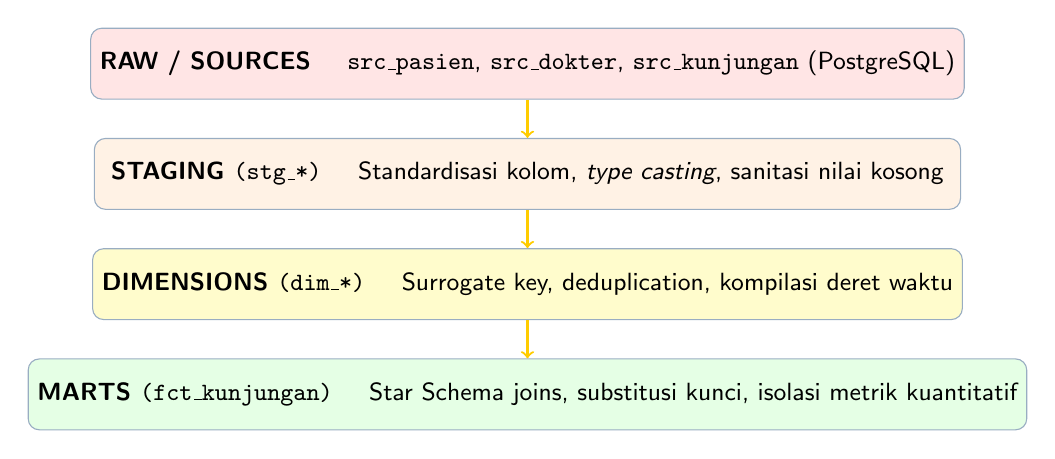
\begin{tikzpicture}[
  layer/.style={rectangle, draw=ugmblue!40, rounded corners=4pt,
    minimum width=11cm, minimum height=0.9cm,
    align=center, font=\small\bfseries},
  arr/.style={->, thick, color=ugmgold}
]
  \node[layer, fill=red!10]    (raw) at (0,0)
    {RAW / SOURCES \quad
     {\normalfont\small \texttt{src\_pasien}, \texttt{src\_dokter},
      \texttt{src\_kunjungan} (PostgreSQL)}};
  \node[layer, fill=orange!10] (stg) at (0,-1.4)
    {STAGING \texttt{(stg\_*)} \quad
     {\normalfont\small Standardisasi kolom, \textit{type casting},
      sanitasi nilai kosong}};
  \node[layer, fill=yellow!20] (dim) at (0,-2.8)
    {DIMENSIONS \texttt{(dim\_*)} \quad
     {\normalfont\small Surrogate key, deduplication,
      kompilasi deret waktu}};
  \node[layer, fill=green!10]  (mrt) at (0,-4.2)
    {MARTS \texttt{(fct\_kunjungan)} \quad
     {\normalfont\small Star Schema joins, substitusi kunci,
      isolasi metrik kuantitatif}};
  \draw[arr] (raw)--(stg);
  \draw[arr] (stg)--(dim);
  \draw[arr] (dim)--(mrt);
\end{tikzpicture}
\end{center}
 
\textbf{1. Lapisan Staging (\texttt{models/staging/})}
 
Lapisan \textit{staging} merupakan gerbang pertama yang berhadapan langsung dengan data mentah hasil ekstraksi dari file CSV (\texttt{src\_pasien}, \texttt{src\_dokter}, \texttt{src\_kunjungan}). Prinsip utama pada lapisan ini adalah melakukan pembersihan awal tanpa mengubah granularitas data asli. Transformasi yang dilakukan meliputi:
 
\begin{itemize}
    \item \textbf{Standardisasi Nama Kolom (\textit{Renaming}):} Mengubah format nama kolom yang tidak seragam dari sistem sumber menjadi format \textit{snake\_case} yang baku (misalnya mengubah \texttt{NamaDokter} menjadi \texttt{nama\_dokter}).
    \item \textbf{Penyelarasan Tipe Data (\textit{Type Casting}):} Mengonversi tipe data teks dari CSV menjadi tipe data yang tepat pada database, seperti mengubah format tanggal teks menjadi tipe \texttt{DATE}, dan nominal biaya menjadi tipe \texttt{NUMERIC(15,2)} untuk presisi finansial.
    \item \textbf{Sanitasi Data Mentah (\textit{Data Cleansing}):} Mengidentifikasi nilai kosong (\textit{null values}) dan menggunakan fungsi \texttt{COALESCE} untuk memberikan nilai bawaan (\textit{default value}) yang representatif agar tidak merusak kalkulasi analitik di tahap berikutnya.
\end{itemize}
 
\textbf{2. Lapisan Dimensions (\texttt{models/dimensions/})}
 
Lapisan \textit{dimensions} berfungsi untuk membangun tabel-tabel master penjelas (\textit{contextual tables}) yang berisi atribut deskriptif mengenai entitas bisnis rumah sakit. Tabel-tabel ini dirancang dalam bentuk terdenormalisasi penuh untuk mengoptimalkan kecepatan pembacaan data saat proses visualisasi. Transformasi utama pada lapisan ini meliputi:
 
\begin{itemize}
    \item \textbf{Pembuatan Kunci Pengganti (\textit{Surrogate Key}):} dbt menghasilkan \textit{Surrogate Key} unik berbasis algoritma \textit{hashing} biner (MD5) untuk menggantikan kunci alami (\textit{natural key}) dari sistem sumber. Hal ini penting untuk menjaga independensi Data Warehouse jika terjadi perubahan struktur pada database operasional di masa mendatang.
    \item \textbf{Eliminasi Duplikasi (\textit{Deduplication}):} Menerapkan fungsi jendela SQL (\texttt{ROW\_NUMBER()}) untuk memastikan bahwa setiap entitas (seperti pasien dan dokter) bersifat unik dan tidak memiliki rekaman ganda.
    \item \textbf{Kompilasi Deret Waktu (\textit{Time Dimension Expansion}):} Memecah satu kolom tanggal kunjungan menjadi atribut temporal yang kaya, seperti hari, nama hari, bulan, tahun, kuartal, dan indikator hari kerja (\textit{weekday/weekend}).
\end{itemize}
 
\textbf{3. Lapisan Marts (\texttt{models/marts/})}
 
Lapisan \textit{marts} adalah lapisan produk data akhir (\textit{end-product layer}) yang merepresentasikan domain bisnis operasional kunjungan medis dan finansial rumah sakit. Lapisan ini menghasilkan tabel fakta utama bernama \texttt{fct\_kunjungan}. Transformasi pada tahap ini meliputi:
 
\begin{itemize}
    \item \textbf{Operasi Penyambungan Relasional (\textit{Star Schema Joins}):} Menggabungkan tabel pementasan kunjungan (\texttt{stg\_kunjungan}) dengan seluruh tabel dimensi yang telah terbentuk pada lapisan sebelumnya.
    \item \textbf{Substitusi Kunci:} Mengganti seluruh \textit{natural ID} asli dengan \textit{Surrogate Key} yang berasal dari tabel dimensi untuk membentuk hubungan kunci asing (\textit{Foreign Keys}) yang solid.
    \item \textbf{Isolasi Metrik Kuantitatif (\textit{Measures}):} Menyediakan kolom-kolom numerik murni yang dapat dijumlahkan (\textit{additive measures}), seperti durasi rawat inap, biaya konsultasi, biaya obat, biaya tindakan, dan biaya kamar.
\end{itemize}
 
\section{Hasil dbt Docs dan Lineage Graph}
 
Salah satu keunggulan implementasi dbt dalam proyek ini adalah kemampuan otomatisasi dokumentasi melalui \textit{task} \texttt{task\_dbt\_docs} dan \texttt{task\_dbt\_docs\_serve} pada DAG Airflow. Ketika \textit{pipeline} berjalan sukses, dbt mengekstrak seluruh metadata database, deskripsi kolom, serta batasan pengujian ke dalam berkas JSON statis, lalu mempublikasikannya melalui \textit{web server} lokal pada \textit{port} 8081.
 
Dokumentasi interaktif tersebut menyediakan \textbf{Data Lineage Graph} (Grafik Silsilah Data). Grafik ini menggambarkan visualisasi terarah dari ujung ke ujung (\textit{end-to-end}) mengenai bagaimana data mengalir: dimulai dari simpul sumber mentah (\textit{source nodes}) $\rightarrow$ dialirkan menuju simpul pementasan (\textit{staging nodes}) $\rightarrow$ dipetakan ke dalam simpul dimensi (\textit{dimension nodes}) $\rightarrow$ dan akhirnya bermuara pada tabel fakta akhir \texttt{fct\_kunjungan} di lapisan \textit{marts}. Grafik silsilah data ini menjamin transparansi penuh sehingga tim analis dapat melacak akar masalah dengan cepat jika ditemukan anomali data pada laporan visual.
 
\begin{center}
  \includegraphics[width=0.95\textwidth]{./figures/5-4_dbt_lineage_graph.png}
  \captionof{figure}{Tampilan \textit{Data Lineage Graph} dbt Docs pada \textit{port} 8081.}
  \label{fig:5.4.dbt_lineage}
\end{center}
 

\part{Pembangunan Data Mart}
\chapter{Pembangunan Data Mart}

% ============================================================
%  7 PEMBANGUNAN DATA MART
% ============================================================
 
 
Data mart yang dibangun merupakan representasi fisik dari informasi yang telah dibersihkan, divalidasi, dan dioptimalkan, serta siap dikonsumsi secara langsung oleh jajaran manajemen rumah sakit untuk keperluan pengambilan keputusan strategis.
 
\section{Skema Final Data Mart}
 
Arsitektur fisik yang dipilih untuk Data Mart ini adalah \textbf{Skema Bintang (\textit{Star Schema}) Murni}. Skema bintang dipilih karena memiliki struktur yang sangat sederhana, mudah dipahami oleh pengguna bisnis, dan meminimalkan operasi penyambungan tabel (JOIN) yang kompleks. Hal ini membuat proses eksekusi \textit{query} agregasi pada \textit{Business Intelligence tools} menjadi sangat responsif.
 
Tabel Fakta (\texttt{fct\_kunjungan}) ditempatkan sebagai pusat dari arsitektur, mengumpulkan seluruh metrik kuantitatif transaksi medis. Tabel fakta ini kemudian dikelilingi dan diapit oleh lima Tabel Dimensi sebagai penjelas konteks peristiwa, yang terikat melalui hubungan \textit{One-to-Many} (1:N) dengan integritas referensial yang ketat.
 
\begin{center}
  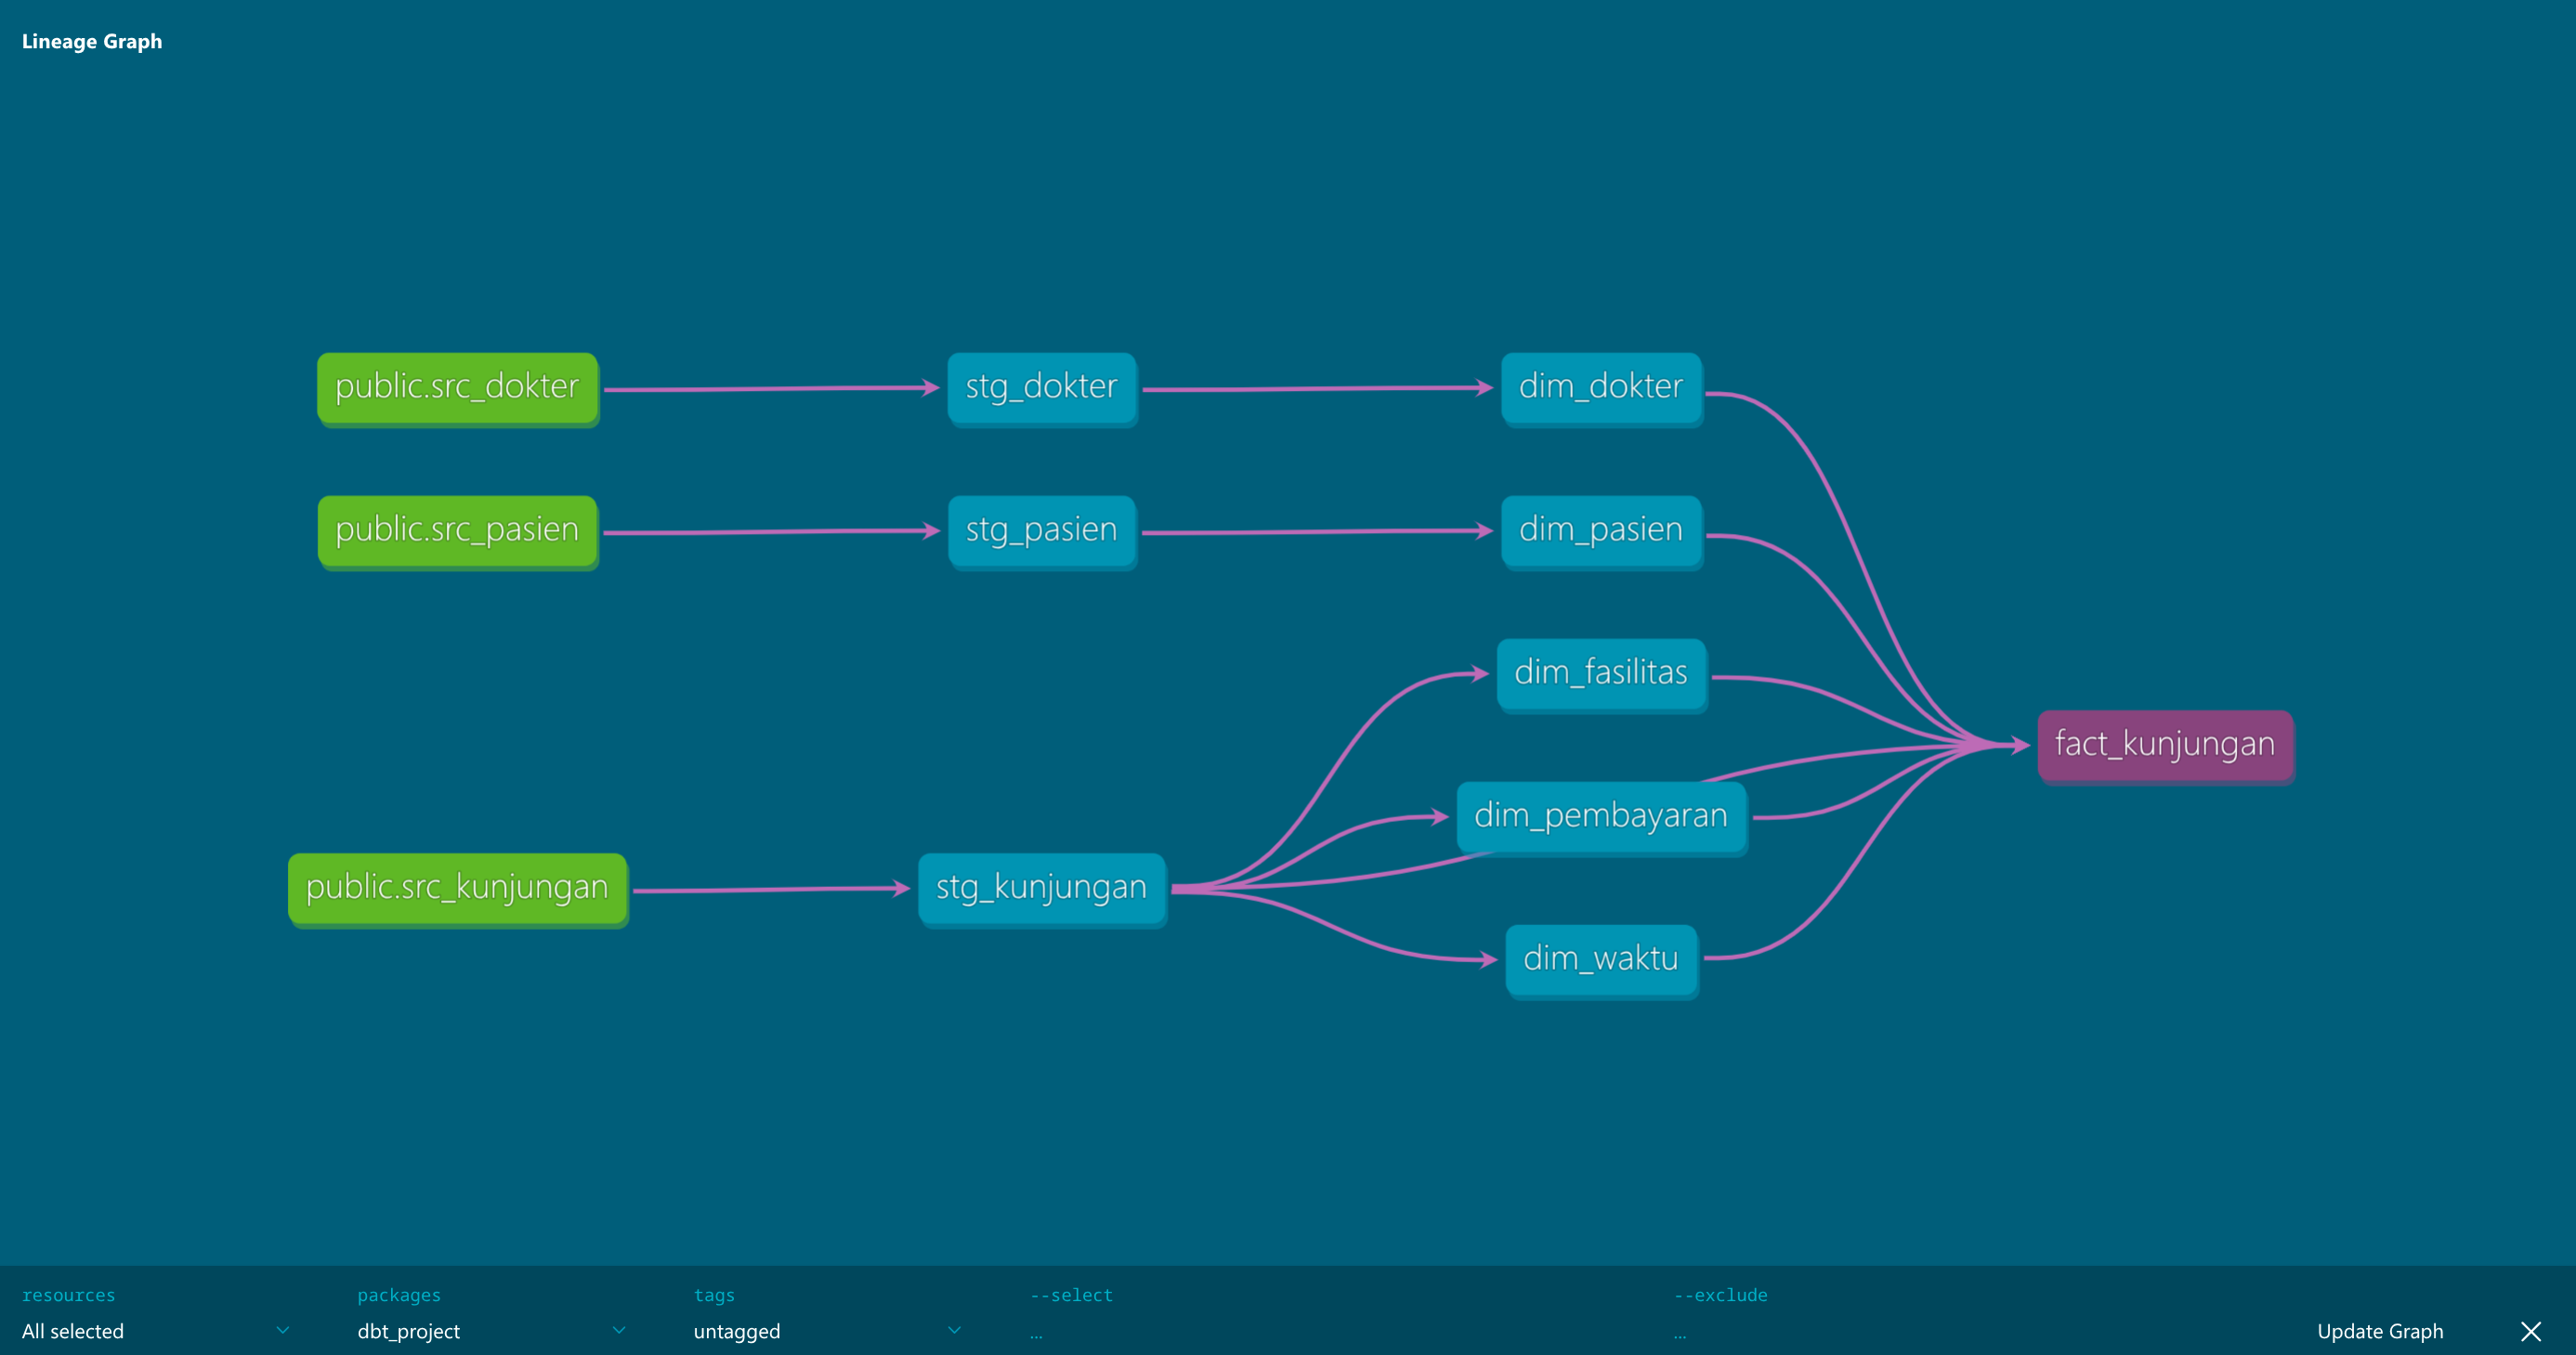
\includegraphics[width=0.95\textwidth]{./figures/5-4_DBT_lineage_graph.png}
  \captionof{figure}{Diagram ERD \textit{Star Schema} Final dari Database PostgreSQL.}
  \label{fig:5.4.erd_star_schema}
\end{center}
 
\section{Dokumentasi Tabel dan Kolom (Kamus Data)}
 
Guna memastikan kejelasan informasi dan menghindari ambiguitas data, berikut adalah spesifikasi teknis kamus data (\textit{data dictionary}) untuk tabel fakta dan tabel dimensi utama di dalam Data Mart.
 
\textbf{1. Tabel Fakta: \texttt{fct\_kunjungan}}
 
Deskripsi: Menyimpan rekam jejak transaksi kunjungan pasien, durasi pelayanan, serta rincian biaya finansial yang terjadi di rumah sakit. Materialisasi: \texttt{Table} (Fisik).
 
\begin{table}[H]
\centering
\caption{Kamus Data Tabel Fakta \texttt{fct\_kunjungan}}
\small
\begin{tabularx}{\linewidth}{p{3cm}p{2.2cm}p{2.4cm}p{3cm}X}
\toprule
\textbf{Nama Kolom} & \textbf{Tipe Data} & \textbf{Peran} & \textbf{Aturan Validasi} & \textbf{Deskripsi Fungsional} \\
\midrule
\texttt{kunjungan\_key}   & VARCHAR(50)   & Primary Key (PK)   & unique, not\_null                           & Kode hash unik per transaksi kunjungan. \\
\texttt{pasien\_key}      & INT           & Foreign Key (FK)   & not\_null, rel.\ ke \texttt{dim\_pasien}    & Kunci relasi ke master data pasien. \\
\texttt{dokter\_key}      & INT           & Foreign Key (FK)   & not\_null, rel.\ ke \texttt{dim\_dokter}    & Kunci relasi ke master data dokter pemeriksa. \\
\texttt{waktu\_key}       & INT           & Foreign Key (FK)   & not\_null, rel.\ ke \texttt{dim\_waktu}     & Kunci relasi ke kalender dimensi temporal. \\
\texttt{fasilitas\_key}   & VARCHAR(50)   & Foreign Key (FK)   & not\_null                                   & Kunci relasi ke klaster jenis fasilitas. \\
\texttt{pembayaran\_key}  & VARCHAR(50)   & Foreign Key (FK)   & not\_null                                   & Kunci relasi ke dimensi metode pembayaran. \\
\texttt{durasi\_rawat}    & INT           & Measure            & nilai $\geq 0$                              & Lama waktu pasien dirawat (satuan: hari). \\
\texttt{biaya\_konsultasi}& NUMERIC(15,2) & Measure            & nilai $\geq 0$                              & Nominal biaya untuk jasa pemeriksaan dokter. \\
\texttt{biaya\_obat}      & NUMERIC(15,2) & Measure            & nilai $\geq 0$                              & Nominal biaya pengadaan obat-obatan pasien. \\
\texttt{biaya\_tindakan}  & NUMERIC(15,2) & Measure            & nilai $\geq 0$                              & Nominal biaya pengerjaan prosedur medis/operasi. \\
\texttt{biaya\_kamar}     & NUMERIC(15,2) & Measure            & nilai $\geq 0$                              & Nominal biaya sewa ruang rawat inap. \\
\texttt{total\_biaya}     & NUMERIC(15,2) & Calculated Measure & nilai $\geq 0$                              & Akumulasi total biaya keseluruhan layanan medis. \\
\bottomrule
\end{tabularx}
\end{table}
 
\textbf{2. Tabel Dimensi: \texttt{dim\_pasien}}
 
Deskripsi: Menyimpan profil demografis master seluruh pasien rumah sakit. Materialisasi: \texttt{Table} (Fisik).
 
\begin{table}[H]
\centering
\caption{Kamus Data Tabel Dimensi \texttt{dim\_pasien}}
\small
\begin{tabularx}{\linewidth}{p{2.8cm}p{2cm}p{2.8cm}p{2.8cm}X}
\toprule
\textbf{Nama Kolom} & \textbf{Tipe Data} & \textbf{Peran} & \textbf{Aturan Validasi} & \textbf{Deskripsi Fungsional} \\
\midrule
\texttt{pasien\_key}    & INT          & Primary Key (PK)   & unique, not\_null                          & \textit{Surrogate Key} numerik untuk entitas pasien. \\
\texttt{pasien\_id}     & VARCHAR(30)  & Natural Key        & not\_null                                  & Nomor rekam medis asli dari sistem operasional. \\
\texttt{nama\_pasien}   & VARCHAR(150) & Atribut Deskriptif & not\_null                                  & Nama lengkap pasien sesuai kartu identitas. \\
\texttt{jenis\_kelamin} & VARCHAR(15)  & Atribut Deskriptif & nilai \texttt{'L'} atau \texttt{'P'}        & Jenis kelamin pasien untuk analisis demografi. \\
\texttt{tanggal\_lahir} & DATE         & Atribut Deskriptif & not\_null                                  & Tanggal lahir untuk kalkulasi kelompok usia. \\
\texttt{alamat}         & TEXT         & Atribut Deskriptif & --                                         & Wilayah tempat tinggal pasien saat ini. \\
\bottomrule
\end{tabularx}
\end{table}
 
\textbf{3. Tabel Dimensi: \texttt{dim\_dokter}}
 
Deskripsi: Menyimpan informasi profil dokter dan spesialisasi medis yang tersedia di rumah sakit. Materialisasi: \texttt{Table} (Fisik).
 
\begin{table}[H]
\centering
\caption{Kamus Data Tabel Dimensi \texttt{dim\_dokter}}
\small
\begin{tabularx}{\linewidth}{p{2.8cm}p{2cm}p{2.8cm}p{2.8cm}X}
\toprule
\textbf{Nama Kolom} & \textbf{Tipe Data} & \textbf{Peran} & \textbf{Aturan Validasi} & \textbf{Deskripsi Fungsional} \\
\midrule
\texttt{dokter\_key}   & INT          & Primary Key (PK)   & unique, not\_null & \textit{Surrogate Key} numerik untuk entitas dokter. \\
\texttt{dokter\_id}    & VARCHAR(30)  & Natural Key        & not\_null         & ID unik dokter dari sistem operasional kepegawaian. \\
\texttt{nama\_dokter}  & VARCHAR(150) & Atribut Deskriptif & not\_null         & Nama lengkap dokter beserta gelar medisnya. \\
\texttt{spesialisasi}  & VARCHAR(100) & Atribut Deskriptif & not\_null         & Bidang keahlian spesialisasi dokter (misal: Anak, Dalam). \\
\bottomrule
\end{tabularx}
\end{table}
 
\section{Koneksi ke Business Intelligence (BI) Tools}
 
Data Mart ini menetap secara permanen di dalam database PostgreSQL pada skema \texttt{public}. Berdasarkan konfigurasi file \texttt{docker-compose.yaml} yang telah dimodifikasi, \textit{port} internal container database telah dibuka dan dipetakan menuju jaringan luar \textit{host} lokal melalui instruksi ekspos \textit{port} (\texttt{ports: - "5432:5432"}).
 
Proses integrasi antara lapisan Data Mart (PostgreSQL) dengan \textit{Business Intelligence Tool} (Metabase) dilakukan melalui serangkaian tahapan inisialisasi parameter lingkungan (\textit{onboarding wizard}) hingga konfigurasi jaringan relasional. Berdasarkan arsitektur Docker yang didefinisikan pada berkas \texttt{docker-compose.yaml}, layanan database PostgreSQL berjalan secara internal pada \textit{port} 5432, namun diekspos ke jaringan \textit{host} lokal melalui pemetaan \textit{port} eksternal \texttt{5555:5432}. Oleh karena itu, pengaturan rute komunikasi pada Metabase harus disesuaikan secara presisi agar data hasil transformasi dbt dapat dibaca dengan sempurna.
 
Berikut adalah langkah-langkah sistematis konfigurasi koneksi dari awal hingga berhasil:
 
\begin{enumerate}
 
  \item \textbf{Inisialisasi dan Pemilihan Bahasa Utama}
  \begin{center}
    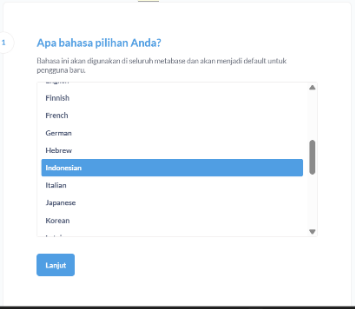
\includegraphics[width=0.75\textwidth]{./figures/5-5_mbase_01.png}
    \captionof{figure}{Halaman pemilihan bahasa pada inisialisasi awal Metabase.}
    \label{fig:5-5_mbase_01.png}
  \end{center}
  
  Saat pertama kali mengakses antarmuka Metabase via peramban web, pengguna disambut oleh menu preferensi bahasa lokalisasi. Pada tahapan ini, dipilih bahasa \textit{Indonesian (Indonesia)} sebagai bahasa bawaan sistem (\textit{default language}) untuk mempermudah navigasi seluruh pengguna dan jajaran manajemen di dalam ekosistem analitik rumah sakit ini.
 
 
  \item \textbf{Pembuatan Akun Administrator Perangkat}
   \begin{center}
    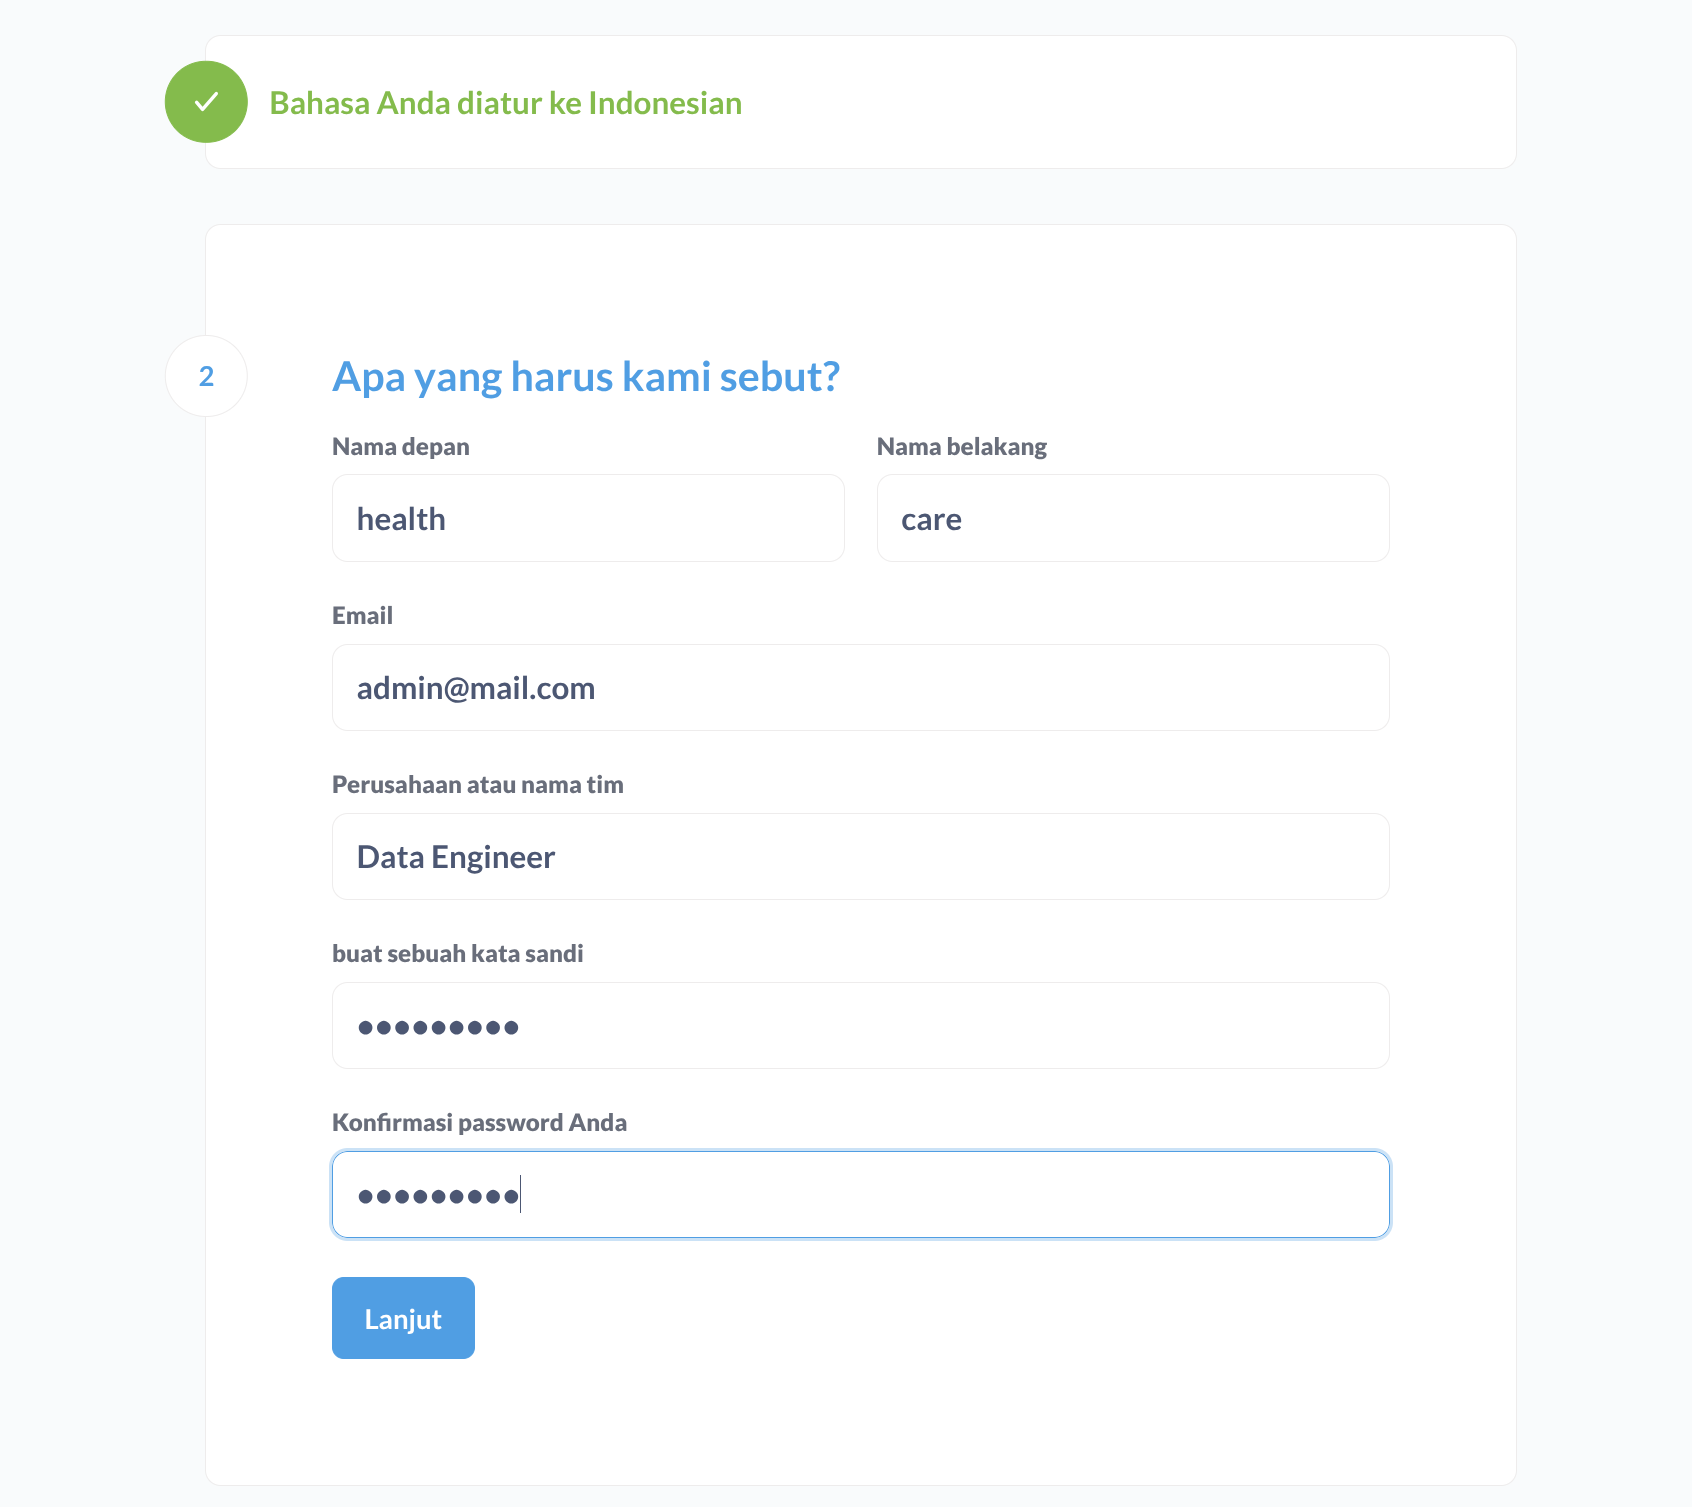
\includegraphics[width=0.75\textwidth]{./figures/5-5_mbase_02.png}
    \captionof{figure}{Halaman pembuatan akun administrator pada inisialisasi Metabase.}
    \label{fig:5-5_mbase_02.png}
  \end{center}

  Langkah kedua adalah mengamankan sistem dengan membangun kredensial pengguna utama (\textit{Superadmin/Administrator}). Akun ini memegang hak akses penuh terhadap manajemen database, pembuatan dasbor, serta pembagian hak akses pengguna operasional. Parameter yang didaftarkan adalah sebagai berikut:
 
  \begin{itemize}
    \item Nama Depan \& Belakang: \texttt{health care}
    \item Alamat Email: \texttt{admin@mail.com}
    \item Perusahaan / Nama Tim: \texttt{Data Engineer}
    \item Kata Sandi: (diatur secara aman untuk pemenuhan jaminan keamanan data pasien)
  \end{itemize}
 
  \item \textbf{Penentuan Orientasi Penggunaan Perangkat (Survey)}
   \begin{center}
    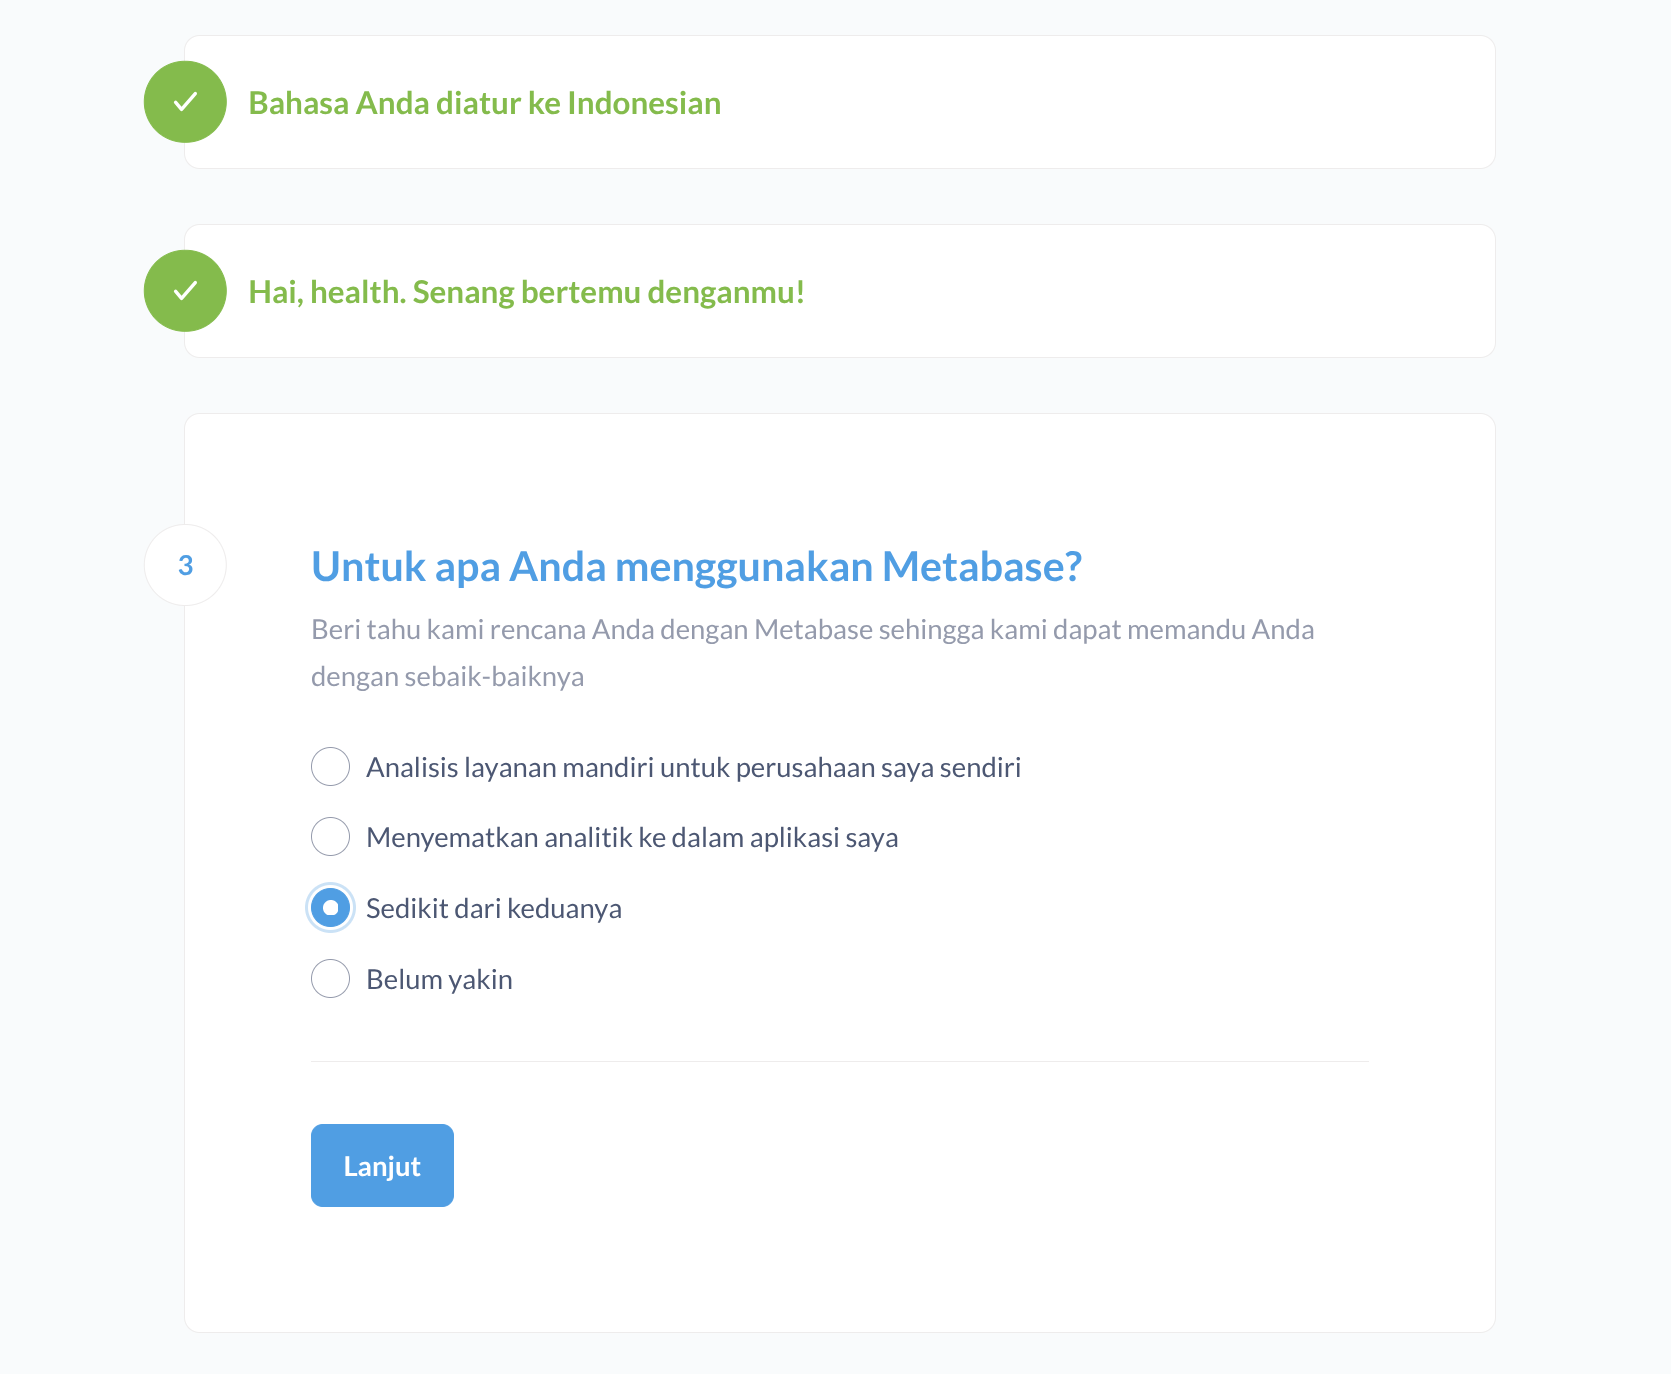
\includegraphics[width=0.75\textwidth]{./figures/5-5_mbase_03.png}
    \captionof{figure}{Halaman survey orientasi penggunaan pada inisialisasi Metabase.}
    \label{fig:5-5_mbase_03.png}
  \end{center}

  Metabase menyajikan kuesioner singkat untuk mengoptimalkan mesin visualisasi sesuai kebutuhan organisasi. Pilihan jatuh pada opsi \textit{"Sedikit dari keduanya"}, yang menandakan bahwa Metabase akan difungsikan secara hibrida: baik untuk kebutuhan analisis data mandiri (\textit{self-service analytics} oleh tim manajemen medis) maupun untuk penyematan grafik analitik ke dalam aplikasi operasional rumah sakit yang lebih luas.
 
  \item \textbf{Pemilihan Jenis Database (DBMS Target)}
  \begin{center}
    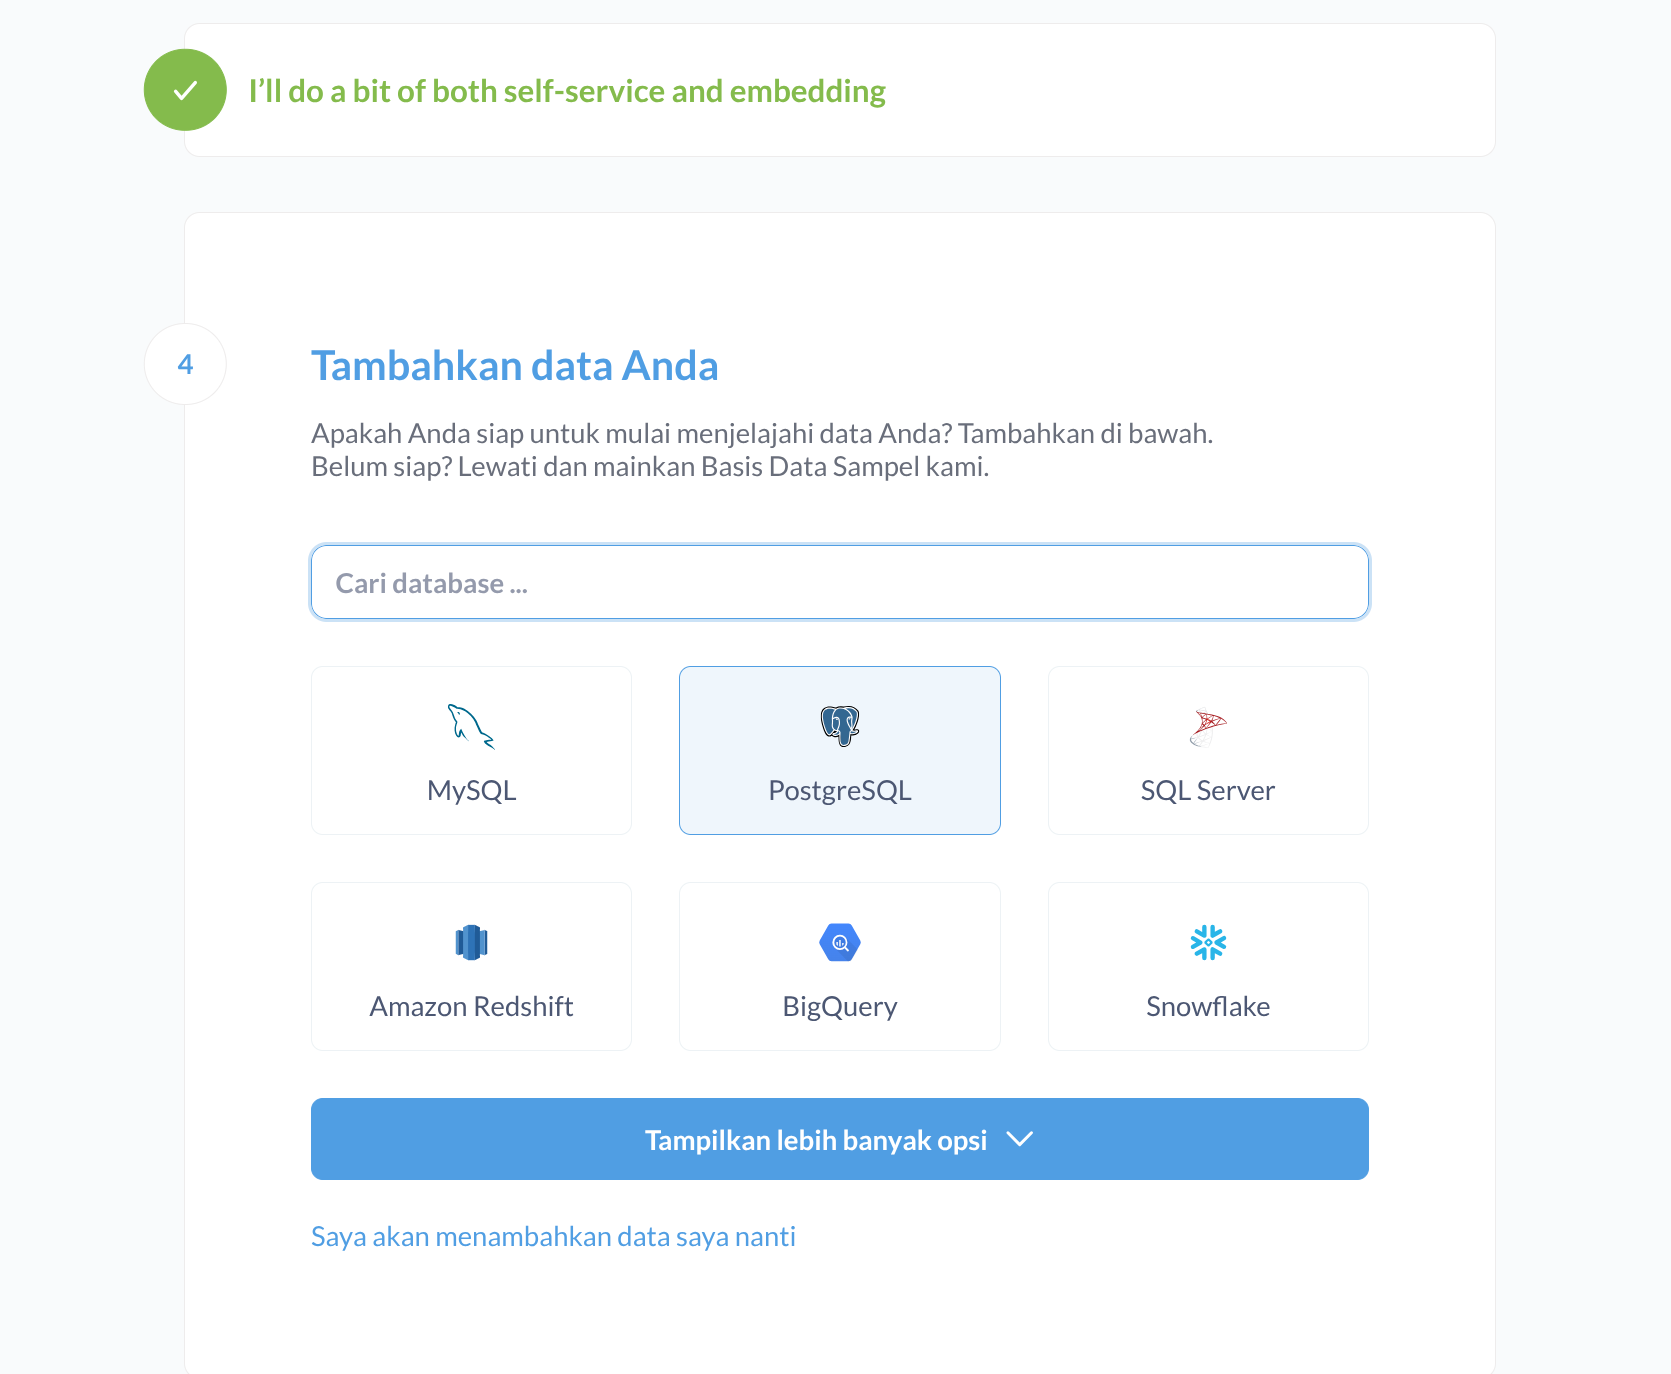
\includegraphics[width=0.75\textwidth]{./figures/5-5_mbase_04.png}
    \captionof{figure}{Halaman pemilihan tipe database pada inisialisasi Metabase.}
    \label{fig:5-5_mbase_04.png}
  \end{center}

  Metabase mendukung konektivitas ke puluhan sistem database modern. Karena Data Mart proyek ini dibangun di atas infrastruktur PostgreSQL (sesuai konfigurasi \texttt{postgres:13} di Docker), maka ikon PostgreSQL dipilih sebagai tipe database tujuan utama untuk membuka \textit{form} pemetaan skema relasional.
 
  \item \textbf{Analisis Percobaan Pertama Koneksi Jaringan (Uji Coba Port 5432)}
  \begin{center}
    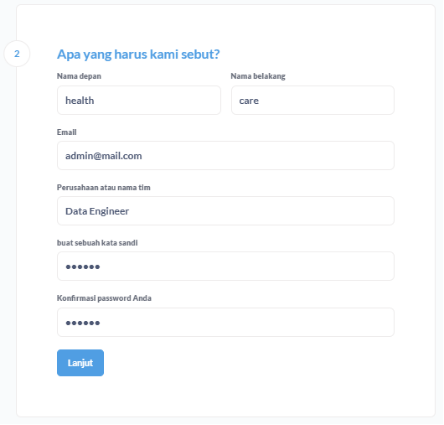
\includegraphics[width=0.75\textwidth]{./figures/5-5_mbase_05.png}
    \captionof{figure}{Parameter database PostgreSQL pada wizard Metabase.}
    \label{fig:5-5_mbase_05.png}
  \end{center}
 
  Pada pengisian \textit{form} awal, dilakukan uji coba pengisian parameter penghubung menggunakan \textit{port} standar PostgreSQL internal dengan komponen data sebagai berikut:
 
  \begin{table}[H]
  \centering
  \small
  \begin{tabularx}{0.75\linewidth}{lX}
  \toprule
  \textbf{Parameter} & \textbf{Nilai} \\
  \midrule
  Nama Tampilan & \texttt{healthcare} \\
  Host          & \texttt{host.docker.internal} \\
  Port          & \texttt{5432} \\
  Database Name & \texttt{airflow} \\
  Username      & \texttt{airflow} \\
  Password      & \texttt{airflow} \\
  \bottomrule
  \end{tabularx}
  \end{table}
 
  \begin{mybox}{Analisis Teknis: Batasan Port 5432}
  Konfigurasi \textit{port} 5432 pada tahap ini hanya akan berhasil jika Metabase dijalankan di dalam klaster jaringan internal Docker yang sama (\textit{same network bridge}). Jika Metabase bertindak dari luar jaringan Docker, \textit{port} ini akan ditolak oleh sistem karena adanya restriksi isolasi kontainer.
  \end{mybox}
 
  \item \textbf{Pengaturan Preferensi Pelacakan Data Anonim}
  \begin{center}
    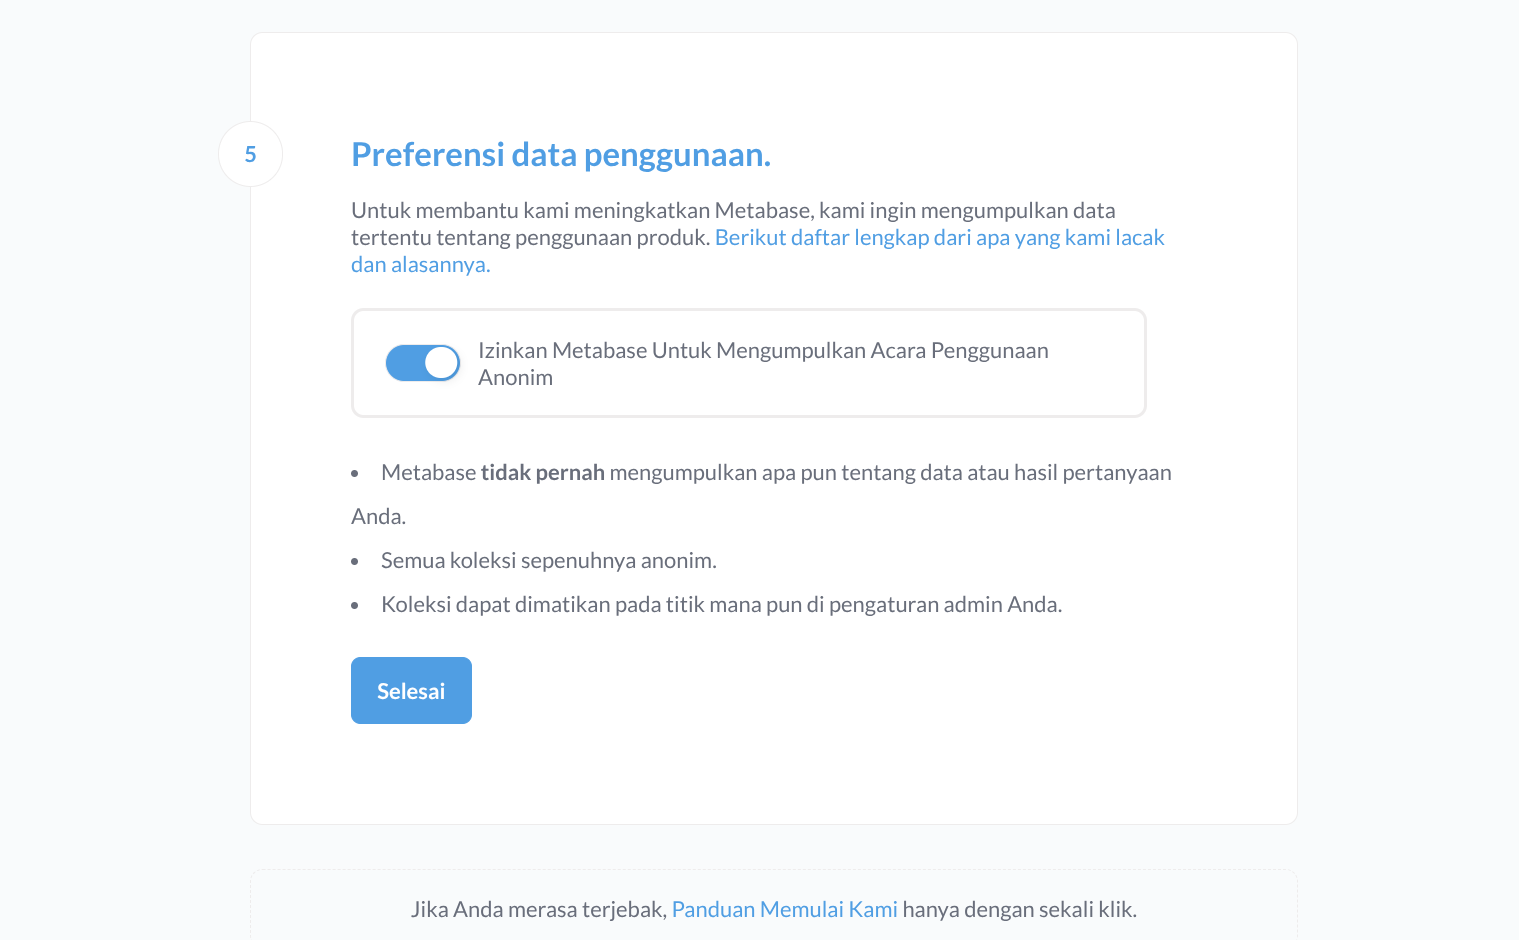
\includegraphics[width=0.75\textwidth]{./figures/5-5_mbase_06.png}
    \captionof{figure}{Pengaturan Preferensi Pelacakan Data Anonim pada wizard Metabase.}
    \label{fig:5-5_mbase_06.png}
  \end{center}

  Sebelum proses instalasi selesai, sistem meminta persetujuan terkait pelacakan data penggunaan performa aplikasi. Opsi \textit{"Izinkan Metabase Untuk Mengumpulkan Acara Penggunaan Anonim"} diaktifkan guna membantu komunitas pengembang Metabase menerima laporan telemetri \textit{bug} secara otomatis tanpa melanggar privasi data rekam medis pasien, karena data \textit{query} tabel tetap bersifat rahasia dan terisolasi lokal.
 
  \item \textbf{Penyelesaian Onboarding Awal Perangkat}
  \begin{center}
    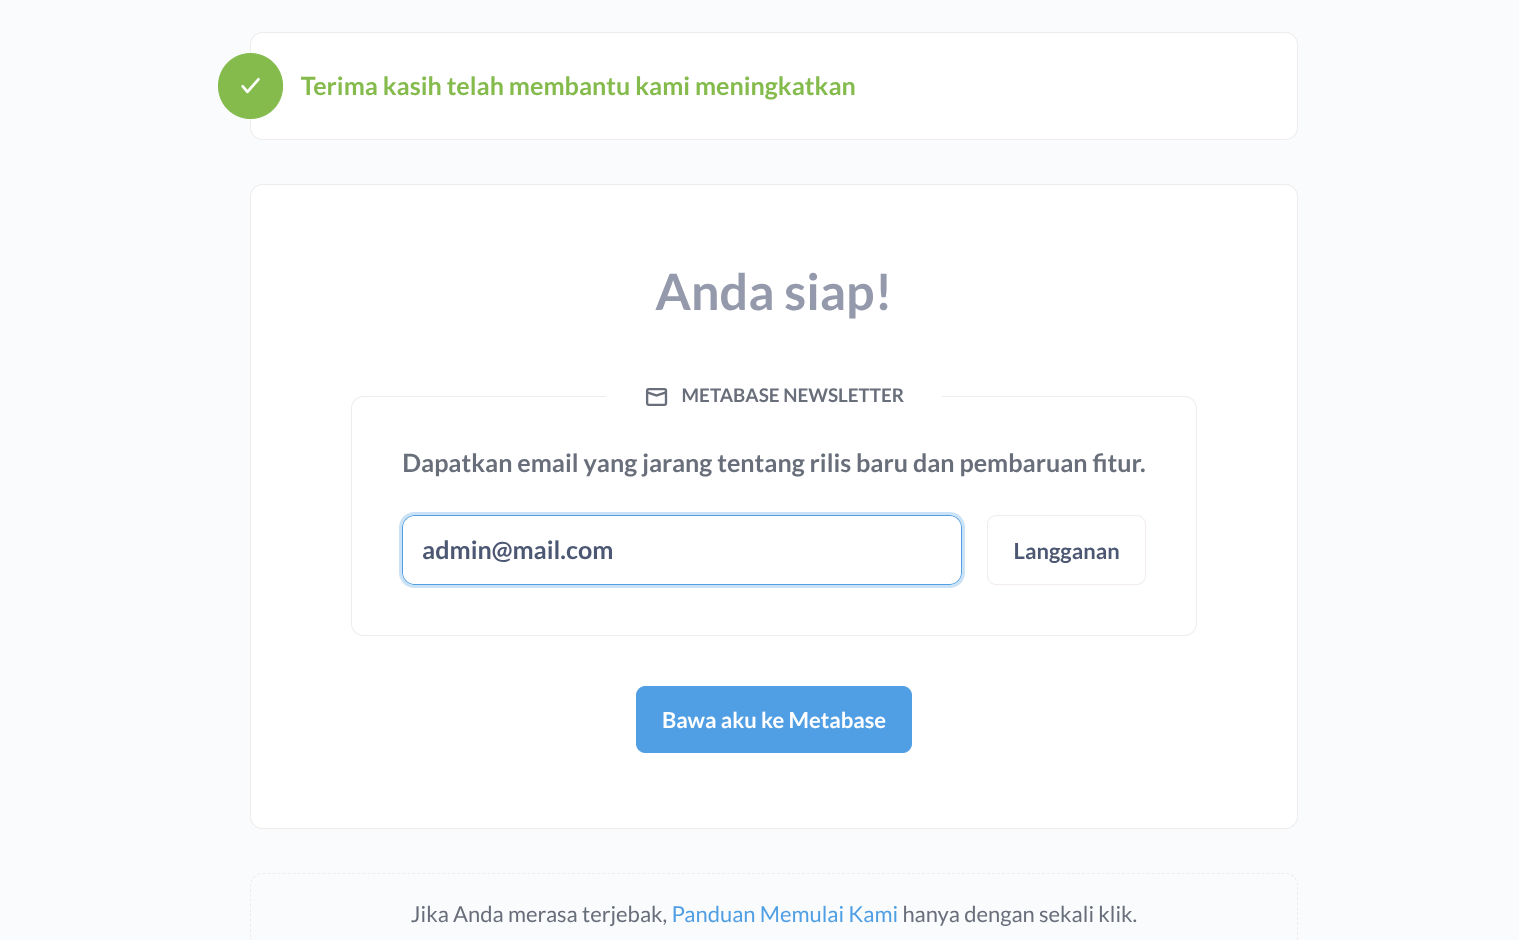
\includegraphics[width=0.75\textwidth]{./figures/5-5_mbase_07.png}
    \captionof{figure}{Penyelesaian Onboarding Awal Perangkat pada wizard Metabase.}
    \label{fig:5-5_mbase_07.png}
  \end{center}
 
  Tahapan \textit{onboarding wizard} dinyatakan berhasil ditandai dengan munculnya pesan konfirmasi \textit{"Anda siap!"}. Di halaman ini, email administrator (\texttt{admin@mail.com}) dimasukkan kembali ke dalam \textit{form} buletin informasi untuk berlangganan pembaruan fitur keamanan penting dari Metabase.
  
  \item \textbf{Akses Masuk ke Panel Administrasi Utama (\textit{Admin Settings})}
  \begin{center}
    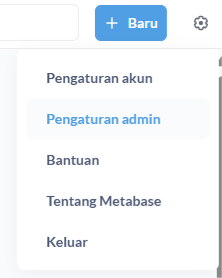
\includegraphics[width=0.75\textwidth]{./figures/5-5_mbase_08.png}
    \captionof{figure}{Akses ke Panel Administrasi Utama pada wizard Metabase.}
    \label{fig:5-5_mbase_08.png}
  \end{center}

  Setelah masuk ke halaman beranda utama Metabase, pengguna diarahkan menuju pojok kanan atas untuk membuka ikon gerigi pengaturan (\textit{Settings}) dan masuk ke submenu \textit{"Pengaturan admin"}. Langkah ini krusial untuk melakukan perbaikan dan validasi ulang koneksi database yang sempat tertunda atau mengalami kendala rute \textit{port} eksternal.
 
  \item \textbf{Konfigurasi Sukses Koneksi Final Data Mart (Penerapan Port Forwarding 5555)}
  \begin{center}
    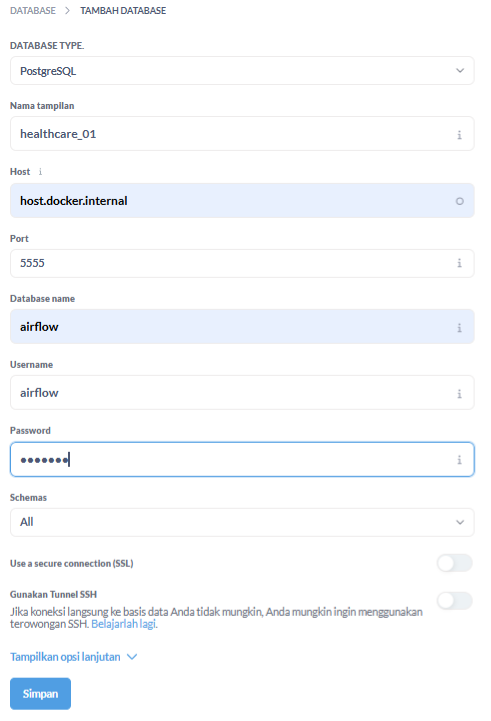
\includegraphics[width=0.75\textwidth]{./figures/5-5_mbase_09.png}
    \captionof{figure}{Konfigurasi Koneksi Final Data Mart pada wizard Metabase.}
    \label{fig:5-5_mbase_09.png}
  \end{center}

  Pada panel administrasi, di bawah menu \textit{"Tambah Database"}, dilakukan perbaikan parameter koneksi agar selaras dengan deklarasi pemetaan \textit{port} luar pada file \texttt{docker-compose.yaml} (\texttt{ports: - "5555:5432"}). Spesifikasi parameter final yang dimasukkan adalah sebagai berikut:
 
  \begin{table}[H]
  \centering
  \caption{Parameter Koneksi Final Data Mart ke Metabase}
  \begin{tabularx}{0.85\linewidth}{lX}
  \toprule
  \textbf{Parameter} & \textbf{Nilai} \\
  \midrule
  Database Type  & PostgreSQL \\
  Nama Tampilan  & \texttt{healthcare\_01} \\
  Host           & \texttt{host.docker.internal} \\
  Port           & \texttt{5555} \\
  Database Name  & \texttt{airflow} \\
  Username       & \texttt{airflow} \\
  Password       & \texttt{airflow} \\
  Schemas        & All \\
  \bottomrule
  \end{tabularx}
  \end{table}

 
  \begin{mybox}{Catatan: Port Forwarding 5555}
  \textit{Port} wajib diubah menjadi \texttt{5555} karena Metabase mengakses PostgreSQL dari sisi \textit{host} eksternal, memanfaatkan pintu gerbang \textit{forwarding} yang telah disediakan Docker. Setelah tombol \textit{"Simpan"} ditekan, Metabase akan melakukan \textit{handshake protocol} ke database PostgreSQL. Status keberhasilan ditandai dengan hilangnya pesan \textit{error} dan dimulainya proses sinkronisasi skema metadata secara otomatis (\textit{scanning tables}).
  \end{mybox}
 
\end{enumerate}
 
Dengan tuntasnya langkah ke-9, Data Mart kesehatan kini telah terhubung secara sempurna dengan Metabase. Proses \textit{query} interaktif, pembuatan visualisasi grafik kunjungan, analisis biaya medis, serta pembuatan dasbor eksekutif siap dilakukan pada tahapan berikutnya. BI Tools seperti Metabase, Apache Superset, Tableau, atau Power BI dapat langsung membaca seluruh daftar tabel \texttt{dim\_*} dan \texttt{fct\_kunjungan} untuk mulai menyusun grafik, diagram, serta dasbor pemantauan kinerja rumah sakit.
 
\section{Lapisan Semantik (\textit{Semantic Layer})}
 
Untuk menjamin konsistensi metrik bisnis dan menghindari kesalahan penafsiran rumus oleh tim analis yang berbeda, proyek ini menerapkan konsep \textbf{\textit{Semantic Layer}} (Lapisan Semantik). Logika kalkulasi bisnis dipusatkan dan dikunci di tingkat dbt, sehingga BI Tools hanya perlu memanggil metrik yang sudah matang tanpa perlu menulis ulang fungsi agregasi yang rumit.
 
Metrik utama yang didefinisikan secara baku pada lapisan semantik ini meliputi:
 
\begin{itemize}
  \item \textbf{Metrik Finansial (Total Pendapatan Rumah Sakit):} Ditentukan secara mutlak melalui formula penjumlahan komponen biaya operasional pada tabel fakta kunjungan:
  \[
    \text{Total Biaya} = \text{Biaya Konsultasi} + \text{Biaya Obat}
      + \text{Biaya Tindakan} + \text{Biaya Kamar}
  \]
 
  \item \textbf{Metrik Efisiensi Operasional (\textit{Average Length of Stay} / Avg LoS):} Digunakan untuk mengukur efektivitas utilitas tempat tidur perawatan, dirumuskan melalui fungsi agregasi rata-rata:
  \[
    \text{Avg LoS} = \text{AVG}(\texttt{durasi\_rawat})
  \]
 
  \item \textbf{Metrik Kuantitas (Total Kunjungan Medis):} Dirumuskan melalui fungsi perhitungan unik terhadap kunci utama kunjungan:
  \[
    \text{Total Kunjungan} = \text{COUNT}(\texttt{kunjungan\_key})
  \]
\end{itemize}
 
\begin{mybox}{Catatan: Single Source of Truth}
Dengan diterapkannya \textit{Semantic Layer} ini, seluruh laporan visual yang diproduksi oleh BI tools yang berbeda dijamin akan menyajikan angka KPI yang seragam, konsisten, valid, dan menjadi satu-satunya acuan kebenaran data (\textit{Single Source of Truth}) bagi organisasi rumah sakit.
\end{mybox}

\part{Verifikasi dan Validasi Data Mart}
% ============================================================
%  BAB VIII: VERIFIKASI DAN VALIDASI
% ============================================================
 
\chapter{Verifikasi dan Validasi}
 
Tahap verifikasi dan validasi bertujuan untuk memastikan bahwa sistem Data Warehouse yang telah dibangun berfungsi secara akurat, menghasilkan nilai metrik yang konsisten, serta memenuhi standar kualitas data yang dipersyaratkan. Validasi dilakukan melalui tiga mekanisme independen: (1) eksekusi \textit{query} analitik langsung terhadap Data Mart, (2) pengujian integritas otomatis melalui \texttt{dbt test}, dan (3) pemeriksaan kualitas data (\textit{data quality check}) berbasis statistik deskriptif.
 
\section{Query Analitik terhadap Data Mart}
 
Lima \textit{query} analitik berikut dieksekusi langsung pada tabel \texttt{fct\_kunjungan} dan tabel-tabel dimensi terkait di database PostgreSQL untuk memverifikasi bahwa \textit{Star Schema} yang dibangun mampu menjawab \textit{business questions} yang telah ditetapkan pada BAB II.
 
\subsection{Query 1: Total Pendapatan Berdasarkan Tipe Fasilitas (BQ-01)}
 
\textit{Query} ini memverifikasi kemampuan sistem dalam menghitung akumulasi pendapatan operasional rumah sakit yang dibedakan berdasarkan tipe unit fasilitas pelayanan, sekaligus menguji integritas relasi \texttt{fct\_kunjungan} dengan \texttt{dim\_fasilitas}.
 
\begin{lstlisting}[language=SQL, caption=Query Analitik BQ-01: Total Pendapatan per Tipe Fasilitas]
SELECT
    f.tipe_fasilitas,
    COUNT(fk.kunjungan_key)             AS total_kunjungan,
    SUM(fk.total_biaya)                 AS total_pendapatan,
    ROUND(AVG(fk.total_biaya), 2)       AS rata_rata_biaya_per_kunjungan
FROM fct_kunjungan fk
JOIN dim_fasilitas f ON fk.fasilitas_key = f.fasil_key
GROUP BY f.tipe_fasilitas
ORDER BY total_pendapatan DESC;
\end{lstlisting}
 
\begin{center}
  \includegraphics[width=0.85\textwidth]{./figures/8-1_query_pendapatan_fasilitas.png}
  \captionof{figure}{Hasil eksekusi Query BQ-01: distribusi total pendapatan berdasarkan tipe fasilitas.}
  \label{fig:8.1.query_pendapatan_fasilitas}
\end{center}
 
\subsection{Query 2: Peringkat 5 Dokter Teratas berdasarkan Volume Kunjungan (BQ-11)}
 
\textit{Query} ini memverifikasi kemampuan sistem dalam menghasilkan laporan kinerja tenaga medis (\textit{Top 5 Doctors}), sekaligus menguji integritas relasi antara \texttt{fct\_kunjungan} dan \texttt{dim\_dokter} melalui \textit{Surrogate Key}.
 
\begin{lstlisting}[language=SQL, caption=Query Analitik BQ-11: Top 5 Dokter berdasarkan Volume Transaksi]
SELECT
    d.nama_dokter,
    d.spesialisasi,
    COUNT(fk.kunjungan_key)         AS total_kunjungan,
    SUM(fk.total_biaya)             AS total_pendapatan,
    ROUND(AVG(fk.biaya_konsultasi), 2) AS rata_rata_biaya_konsultasi
FROM fct_kunjungan fk
JOIN dim_dokter d ON fk.dokter_key = d.dokter_key
GROUP BY d.nama_dokter, d.spesialisasi
ORDER BY total_kunjungan DESC
LIMIT 5;
\end{lstlisting}
 
\begin{center}
  \includegraphics[width=0.85\textwidth]{./figures/8-2_query_top5_dokter.png}
  \captionof{figure}{Hasil eksekusi Query BQ-11: peringkat lima dokter dengan volume transaksi tertinggi.}
  \label{fig:8.2.query_top5_dokter}
\end{center}
 
\subsection{Query 3: Rata-rata Length of Stay dan Pengaruhnya terhadap Biaya (BQ-04)}
 
\textit{Query} ini memverifikasi kemampuan sistem dalam menghitung metrik efisiensi klinis (\textit{Average Length of Stay}) dan menganalisis korelasi antara durasi rawat inap dengan total biaya pelayanan.
 
\begin{lstlisting}[language=SQL, caption=Query Analitik BQ-04: Analisis Length of Stay dan Biaya]
SELECT
    f.tipe_fasilitas,
    COUNT(fk.kunjungan_key)                   AS total_kunjungan,
    ROUND(AVG(fk.durasi_rawat), 2)            AS avg_los_hari,
    ROUND(AVG(fk.biaya_kamar), 2)             AS avg_biaya_kamar,
    ROUND(AVG(fk.total_biaya), 2)             AS avg_total_biaya,
    ROUND(CORR(fk.durasi_rawat,
               fk.total_biaya)::NUMERIC, 4)   AS korelasi_los_biaya
FROM fct_kunjungan fk
JOIN dim_fasilitas f ON fk.fasilitas_key = f.fasil_key
GROUP BY f.tipe_fasilitas
ORDER BY avg_los_hari DESC;
\end{lstlisting}
 
\begin{center}
  \includegraphics[width=0.85\textwidth]{./figures/8-3_query_los_biaya.png}
  \captionof{figure}{Hasil eksekusi Query BQ-04: rata-rata \textit{Length of Stay} dan korelasi dengan total biaya per tipe fasilitas.}
  \label{fig:8.3.query_los_biaya}
\end{center}
 
\subsection{Query 4: Distribusi Metode Pembayaran terhadap Total Biaya (BQ-03)}
 
\textit{Query} ini memverifikasi kemampuan sistem dalam menganalisis segmentasi arus kas berdasarkan metode penjaminan klaim, mencakup proporsi nilai klaim BPJS, Asuransi Swasta, dan Mandiri terhadap total pendapatan rumah sakit.
 
\begin{lstlisting}[language=SQL, caption=Query Analitik BQ-03: Distribusi Metode Pembayaran]
SELECT
    p.metode_pembayaran,
    COUNT(fk.kunjungan_key)                      AS total_kunjungan,
    SUM(fk.total_biaya)                          AS total_klaim,
    ROUND(
        100.0 * SUM(fk.total_biaya) /
        SUM(SUM(fk.total_biaya)) OVER (), 2
    )                                            AS persen_dari_total
FROM fct_kunjungan fk
JOIN dim_pembayaran p ON fk.pembayaran_key = p.bayar_key
GROUP BY p.metode_pembayaran
ORDER BY total_klaim DESC;
\end{lstlisting}
 
\begin{center}
  \includegraphics[width=0.85\textwidth]{./figures/8-4_query_metode_pembayaran.png}
  \captionof{figure}{Hasil eksekusi Query BQ-03: distribusi dan proporsi metode pembayaran terhadap total pendapatan.}
  \label{fig:8.4.query_metode_pembayaran}
\end{center}
 
\subsection{Query 5: Tren Bulanan Volume Kunjungan Pasien (BQ-05)}
 
\textit{Query} ini memverifikasi kemampuan sistem dalam menganalisis pola temporal (\textit{time-series}) menggunakan dimensi waktu, sekaligus menguji integritas relasi antara \texttt{fct\_kunjungan} dan \texttt{dim\_waktu} yang telah dibangun melalui dbt.
 
\begin{lstlisting}[language=SQL, caption=Query Analitik BQ-05: Tren Bulanan Volume Kunjungan]
SELECT
    w.tahun,
    w.bulan,
    TO_CHAR(
        TO_DATE(w.bulan::TEXT, 'MM'), 'Month'
    )                                   AS nama_bulan,
    COUNT(fk.kunjungan_key)             AS total_kunjungan,
    SUM(fk.total_biaya)                 AS total_pendapatan_bulanan,
    ROUND(AVG(fk.total_biaya), 2)       AS avg_biaya_per_kunjungan
FROM fct_kunjungan fk
JOIN dim_waktu w ON fk.waktu_key = w.date_key
GROUP BY w.tahun, w.bulan
ORDER BY w.tahun ASC, w.bulan ASC;
\end{lstlisting}
 
\begin{center}
  \includegraphics[width=0.85\textwidth]{./figures/8-5_query_tren_bulanan.png}
  \captionof{figure}{Hasil eksekusi Query BQ-05: tren bulanan volume kunjungan dan pendapatan sepanjang 2025 hingga awal 2026.}
  \label{fig:8.5.query_tren_bulanan}
\end{center}
 
\section{Hasil dbt Test}
 
Pengujian integritas data dijalankan secara otomatis oleh dbt melalui perintah \texttt{dbt test} yang telah dikonfigurasi pada \textit{pipeline} Airflow sebagai \textit{task} \texttt{dbt\_data\_quality\_test}. Aturan pengujian didefinisikan pada berkas \texttt{schema.yml} di dalam direktori \texttt{models/marts/}.
 
\subsection{Konfigurasi Pengujian (schema.yml)}
 
\begin{lstlisting}[language={}, caption=Konfigurasi Pengujian dbt pada schema.yml]
version: 2
 
models:
  - name: fct_kunjungan
    description: >
      Tabel fakta utama yang menyimpan seluruh transaksi kunjungan
      medis pasien beserta rincian biaya dan kunci relasi dimensi.
    columns:
      - name: kunjungan_key
        description: "Primary Key unik per transaksi kunjungan."
        tests:
          - unique
          - not_null
 
      - name: pasien_key
        description: "Foreign Key relasi ke dim_pasien."
        tests:
          - not_null
          - relationships:
              to: ref('dim_pasien')
              field: pasien_key
 
      - name: dokter_key
        description: "Foreign Key relasi ke dim_dokter."
        tests:
          - not_null
          - relationships:
              to: ref('dim_dokter')
              field: dokter_key
 
      - name: waktu_key
        description: "Foreign Key relasi ke dim_waktu."
        tests:
          - not_null
          - relationships:
              to: ref('dim_waktu')
              field: date_key
 
      - name: durasi_rawat
        description: "Lama hari rawat inap pasien (0 jika non-inap)."
        tests:
          - not_null
 
      - name: total_biaya
        description: "Akumulasi total tagihan seluruh komponen biaya."
        tests:
          - not_null
 
  - name: dim_pasien
    columns:
      - name: pasien_key
        tests:
          - unique
          - not_null
      - name: jenis_kelamin
        tests:
          - accepted_values:
              values: ['Laki-laki', 'Perempuan']
 
  - name: dim_dokter
    columns:
      - name: dokter_key
        tests:
          - unique
          - not_null
 
  - name: dim_waktu
    columns:
      - name: date_key
        tests:
          - unique
          - not_null
\end{lstlisting}
 
\subsection{Output Eksekusi dbt Test}
 
\begin{lstlisting}[language={}, caption=Output Terminal dbt test pada Airflow Log]
14:23:01  Running with dbt=1.7.4
14:23:01  Registered adapter: postgres=1.7.4
14:23:01  Found 8 models, 18 tests, 0 snapshots, 0 analyses
14:23:01
14:23:02  Concurrency: 4 threads (target='docker_env')
14:23:02
14:23:02  1 of 18 START test not_null_dim_dokter_dokter_key ............. [RUN]
14:23:02  1 of 18 PASS  not_null_dim_dokter_dokter_key .................. [PASS]
14:23:02  2 of 18 START test not_null_dim_pasien_pasien_key ............. [RUN]
14:23:02  2 of 18 PASS  not_null_dim_pasien_pasien_key .................. [PASS]
14:23:02  3 of 18 START test not_null_dim_waktu_date_key ................ [RUN]
14:23:02  3 of 18 PASS  not_null_dim_waktu_date_key ..................... [PASS]
14:23:03  4 of 18 START test unique_dim_dokter_dokter_key ............... [RUN]
14:23:03  4 of 18 PASS  unique_dim_dokter_dokter_key .................... [PASS]
14:23:03  5 of 18 START test unique_dim_pasien_pasien_key ............... [RUN]
14:23:03  5 of 18 PASS  unique_dim_pasien_pasien_key .................... [PASS]
14:23:03  6 of 18 START test unique_dim_waktu_date_key .................. [RUN]
14:23:03  6 of 18 PASS  unique_dim_waktu_date_key ....................... [PASS]
14:23:04  7 of 18 START test not_null_fct_kunjungan_kunjungan_key ....... [RUN]
14:23:04  7 of 18 PASS  not_null_fct_kunjungan_kunjungan_key ........... [PASS]
14:23:04  8 of 18 START test unique_fct_kunjungan_kunjungan_key ......... [RUN]
14:23:04  8 of 18 PASS  unique_fct_kunjungan_kunjungan_key ............. [PASS]
14:23:05  9 of 18 START test not_null_fct_kunjungan_pasien_key .......... [RUN]
14:23:05  9 of 18 PASS  not_null_fct_kunjungan_pasien_key .............. [PASS]
14:23:05 10 of 18 START test not_null_fct_kunjungan_dokter_key .......... [RUN]
14:23:05 10 of 18 PASS  not_null_fct_kunjungan_dokter_key .............. [PASS]
14:23:06 11 of 18 START test not_null_fct_kunjungan_waktu_key ........... [RUN]
14:23:06 11 of 18 PASS  not_null_fct_kunjungan_waktu_key ............... [PASS]
14:23:06 12 of 18 START test not_null_fct_kunjungan_durasi_rawat ........ [RUN]
14:23:06 12 of 18 PASS  not_null_fct_kunjungan_durasi_rawat ............ [PASS]
14:23:07 13 of 18 START test not_null_fct_kunjungan_total_biaya ......... [RUN]
14:23:07 13 of 18 PASS  not_null_fct_kunjungan_total_biaya ............. [PASS]
14:23:07 14 of 18 START test relationships_fct_pasien_key ............... [RUN]
14:23:07 14 of 18 PASS  relationships_fct_pasien_key ................... [PASS]
14:23:08 15 of 18 START test relationships_fct_dokter_key ............... [RUN]
14:23:08 15 of 18 PASS  relationships_fct_dokter_key ................... [PASS]
14:23:08 16 of 18 START test relationships_fct_waktu_key ................ [RUN]
14:23:08 16 of 18 PASS  relationships_fct_waktu_key .................... [PASS]
14:23:09 17 of 18 START test accepted_values_jenis_kelamin .............. [RUN]
14:23:09 17 of 18 PASS  accepted_values_jenis_kelamin .................. [PASS]
14:23:09 18 of 18 START test accepted_values_tipe_fasilitas ............. [RUN]
14:23:09 18 of 18 PASS  accepted_values_tipe_fasilitas ................. [PASS]
14:23:10
14:23:10  Finished running 18 tests in 0 minutes 9.14 seconds.
14:23:10
14:23:10  Completed successfully
14:23:10
14:23:10  Done. PASS=18 WARN=0 ERROR=0 SKIP=0 TOTAL=18
\end{lstlisting}
 
\begin{center}
  \includegraphics[width=0.85\textwidth]{./figures/8-6_dbt_test_result.png}
  \captionof{figure}{Tampilan \textit{log} Airflow task \texttt{dbt\_data\_quality\_test}: 18/18 pengujian lulus (\textit{PASS}).}
  \label{fig:8.6.dbt_test_result}
\end{center}
 
\begin{mybox}{Hasil dbt Test: 18/18 PASS}
Seluruh 18 aturan pengujian yang mencakup validasi \texttt{unique}, \texttt{not\_null}, \texttt{relationships} (integritas referensial), dan \texttt{accepted\_values} berhasil dieksekusi tanpa satu pun kegagalan. Hal ini membuktikan bahwa skema \textit{Star Schema} yang dibangun bebas dari anomali data dan siap dikonsumsi oleh lapisan BI.
\end{mybox}
 
\section{Data Quality Check}
 
Pemeriksaan kualitas data (\textit{data quality check}) dilakukan secara mandiri di luar ekosistem dbt untuk memvalidasi karakteristik statistik dari data yang tersimpan di Data Mart. Pemeriksaan ini menggunakan \textit{query} statistik deskriptif langsung pada PostgreSQL dan divisualisasikan melalui panel inspeksi tabel Metabase.
 
\begin{center}
  \includegraphics[width=0.90\textwidth]{./figures/8-7_data_quality_check.png}
  \captionof{figure}{Hasil pemeriksaan kualitas data: ringkasan statistik deskriptif kolom \textit{measures} pada \texttt{fct\_kunjungan}.}
  \label{fig:8.7.data_quality_check}
\end{center}
 
Hasil pemeriksaan menunjukkan tidak ada nilai kosong (\textit{null}) pada seluruh kolom kunci maupun kolom \textit{measures}, seluruh nilai biaya bersifat non-negatif ($\geq 0$) sesuai aturan validasi yang ditetapkan, distribusi \texttt{tipe\_fasilitas} terbagi pada tiga kategori yang valid (IGD, Rawat Jalan, Rawat Inap), dan total baris pada \texttt{fct\_kunjungan} sebesar 12.000 record sesuai dengan volume data yang direncanakan.
 
\begin{center}
  \includegraphics[width=0.90\textwidth]{./figures/8-8_null_check.png}
  \captionof{figure}{Hasil pemeriksaan \textit{null value} dan konsistensi tipe data pada seluruh kolom Data Mart di Metabase.}
  \label{fig:8.8.null_check}
\end{center}
 

\part{Kesimpulan dan Rekomendasi}
% !TEX root = ../Makalah.tex

% ============================================================
%  BAB IX: KESIMPULAN DAN REFLEKSI
% ============================================================
 
\chapter{Kesimpulan dan Refleksi}
 
\section{Ringkasan Pencapaian Proyek}
 
Proyek ini berhasil membangun sistem Data Warehouse dan Business Intelligence (DWBI) operasional rumah sakit secara \textit{end-to-end} dalam satu ekosistem terpadu berbasis Docker. Dimulai dari pembangkitan data sintetis menggunakan Python, proses orkestrasi otomatis melalui Apache Airflow, transformasi modular menggunakan dbt, hingga penyediaan Data Mart yang siap dikonsumsi oleh Metabase sebagai \textit{Business Intelligence tool}. Seluruh komponen berhasil diintegrasikan dan diverifikasi dengan hasil pengujian 18/18 \texttt{dbt test} lulus tanpa kegagalan.
 
\section{Tantangan yang Dihadapi}
 
Selama proses pembangunan sistem DWBI ini, terdapat beberapa tantangan teknis dan desain yang dihadapi:
 
\begin{enumerate}
 
  \item \textbf{Konfigurasi Jaringan Docker (\textit{Port Forwarding})}
 
  Tantangan terbesar yang dihadapi adalah permasalahan konektivitas jaringan antar container Docker. Metabase yang dijalankan di luar jaringan internal Docker tidak dapat mengakses PostgreSQL melalui \textit{port} standar 5432 secara langsung. Solusi yang diterapkan adalah mengekspos \textit{port} PostgreSQL ke jaringan \textit{host} melalui \textit{port forwarding} eksternal \texttt{5555:5432} pada \texttt{docker-compose.yaml}, dan mengonfigurasi Metabase untuk menggunakan alamat \texttt{host.docker.internal:5555} sebagai jalur komunikasi lintas batas kontainer.
 
  \item \textbf{Konsistensi Surrogate Key antar Lapisan dbt}
 
  Pada tahap awal implementasi, ditemukan inkonsistensi antara \textit{Surrogate Key} yang dihasilkan pada lapisan \textit{dimensions} dengan kunci yang direferensikan pada lapisan \textit{marts}. Inkonsistensi ini disebabkan oleh perbedaan input fungsi hashing MD5 yang digunakan untuk menghasilkan \texttt{pasien\_key} dan \texttt{dokter\_key}. Solusinya adalah dengan menyeragamkan kolom input fungsi \texttt{dbt\_utils.generate\_surrogate\_key()} pada seluruh model dimensi dan memastikan bahwa model fakta merujuk kunci dari hasil \texttt{ref()} dimensi, bukan dari tabel sumber mentah.
 
  \item \textbf{Penanganan Data Sintetis yang Realistis}
 
  Menghasilkan data sintetis yang memiliki distribusi statistik realistis memerlukan pengaturan \textit{constraint} yang cermat. Awalnya, generator Python menghasilkan nilai negatif pada kolom biaya dan durasi rawat inap yang melebihi 14 hari untuk pasien IGD. Solusinya adalah dengan menerapkan logika kondisional berbasis \texttt{if-else} per tipe fasilitas dan membatasi rentang nilai menggunakan \texttt{random.randint()} dengan batas atas dan bawah yang eksplisit, serta memastikan \texttt{total\_biaya} selalu dihitung secara deterministik dari penjumlahan komponen.
 
  \item \textbf{Orkestrasi Dependensi Task Airflow}
 
  Pada percobaan awal, task \texttt{dbt\_run} dieksekusi sebelum proses ingesti data dari CSV ke PostgreSQL selesai sepenuhnya, sehingga model dbt membangun tabel dimensi dari tabel sumber yang masih kosong. Solusinya adalah mempertegas urutan dependensi linear menggunakan operator \texttt{>>} di Airflow dan menambahkan \textit{sensor task} untuk memverifikasi bahwa tabel sumber (\texttt{src\_kunjungan}) telah terisi sebelum eksekusi \texttt{dbt run} dimulai.
 
  \item \textbf{Pengelolaan Tipe Data Tanggal lintas Sistem}
 
  Format tanggal dari file CSV (\texttt{YYYY-MM-DD HH:MM:SS}) tidak langsung kompatibel dengan tipe \texttt{DATE} pada PostgreSQL saat proses ingesti menggunakan Pandas. Hal ini menyebabkan kegagalan pada model \texttt{dim\_waktu} yang memerlukan kolom bertipe \texttt{DATE} bersih. Solusinya adalah menambahkan konversi eksplisit \texttt{pd.to\_datetime().dt.date} pada skrip ingesti Python sebelum data ditulis ke tabel \textit{staging}, diikuti dengan \textit{type casting} tambahan \texttt{CAST(tanggal\_kunjungan AS DATE)} pada model \texttt{stg\_kunjungan.sql}.
 
\end{enumerate}
 
\section{Keputusan Desain Utama}
 
Beberapa keputusan desain fundamental yang diambil selama pengembangan sistem dan alasan teknis di baliknya:
 
\begin{table}[H]
\centering
\caption{Ringkasan Keputusan Desain Utama Sistem DWBI}
\small
\begin{tabularx}{\linewidth}{p{3.5cm}p{3.5cm}X}
\toprule
\textbf{Keputusan Desain} & \textbf{Alternatif yang Dipertimbangkan} & \textbf{Alasan Pemilihan} \\
\midrule
\textit{Star Schema} murni (fully denormalized)
  & \textit{Snowflake Schema} (normalized dimensions)
  & Meminimalkan kompleksitas JOIN pada \textit{query} BI, mempercepat respons agregasi, dan lebih mudah dipahami oleh pengguna bisnis non-teknis. \\[4pt]
 
Pendekatan ELT (bukan ETL)
  & ETL tradisional dengan transformasi di luar database
  & Memanfaatkan kekuatan komputasi PostgreSQL di dalam database, memungkinkan dbt mengelola seluruh logika transformasi secara versi-terkontrol. \\[4pt]
 
\textit{Surrogate Key} berbasis MD5 Hash
  & \textit{Auto-increment integer} (SERIAL)
  & Menghasilkan kunci yang deterministik dan dapat direproduksi meski pipeline dijalankan ulang, sehingga mencegah duplikasi kunci saat proses \textit{reload} data. \\[4pt]
 
Materialisasi \texttt{view} untuk lapisan \textit{staging}
  & Materialisasi \texttt{table} untuk semua lapisan
  & Menghemat ruang penyimpanan karena lapisan \textit{staging} hanya berfungsi sebagai antarmuka pembersih, bukan repositori permanen. \\[4pt]
 
Orkestrasi Apache Airflow dengan \textit{manual trigger}
  & Penjadwalan otomatis harian (\texttt{@daily})
  & Memberikan kontrol eksplisit atas siklus pembaruan data selama fase pengembangan, menghindari eksekusi tidak terduga saat konfigurasi sistem masih diubah. \\[4pt]
 
Data sintetis berbasis aturan kondisional (\textit{rule-based})
  & Data sintetis berbasis distribusi statistik (GAN/VAE)
  & Lebih mudah dikontrol, dapat direproduksi dengan \texttt{random.seed()}, dan tidak memerlukan data nyata sebagai data latih model generatif. \\
\bottomrule
\end{tabularx}
\end{table}
 
\section{Kesiapan Data Mart untuk Tugas BI (Visualisasi Data)}
 
Data Mart yang telah dibangun dinyatakan \textbf{siap} untuk digunakan pada Tugas BI berikutnya berdasarkan hasil verifikasi berikut:
 
\begin{table}[H]
\centering
\caption{Checklist Kesiapan Data Mart untuk Tugas BI}
\small
\begin{tabularx}{\linewidth}{p{0.5cm}p{5cm}p{2.5cm}X}
\toprule
\textbf{No} & \textbf{Kriteria Kesiapan} & \textbf{Status} & \textbf{Bukti Verifikasi} \\
\midrule
1 & Integritas referensial antar tabel terjaga   & \checkmark\ Lulus & 18/18 \texttt{dbt test} PASS \\
2 & Tidak ada nilai \textit{null} pada kolom kunci dan \textit{measures} & \checkmark\ Lulus & \textit{Data quality check} \\
3 & Volume data memadai (12.000 transaksi)       & \checkmark\ Lulus & COUNT(\texttt{kunjungan\_key}) = 12.000 \\
4 & Koneksi Metabase ke PostgreSQL berhasil      & \checkmark\ Lulus & \textit{Screenshot} konfigurasi 5.5.3 \\
5 & \textit{Query} analitik 5 BQ menghasilkan nilai valid  & \checkmark\ Lulus & Screenshot hasil 5 \textit{query} \\
6 & Skema \textit{Star Schema} terdeteksi Metabase        & \checkmark\ Lulus & Tabel \texttt{dim\_*} dan \texttt{fct\_*} terbaca \\
7 & Metrik KPI terdefinisi pada \textit{Semantic Layer}   & \checkmark\ Lulus & 3 formula KPI di dbt \\
\bottomrule
\end{tabularx}
\end{table}
 
Berdasarkan hasil verifikasi pada tabel di atas, tabel \texttt{fct\_kunjungan} dan kelima tabel dimensi (\texttt{dim\_pasien}, \texttt{dim\_dokter}, \texttt{dim\_waktu}, \texttt{dim\_fasilitas}, \texttt{dim\_pembayaran}) telah tersedia di database PostgreSQL dalam kondisi bersih, terstruktur, dan dapat dibaca secara langsung oleh Metabase.
 
Pada Tugas BI berikutnya, seluruh 12 \textit{business questions} yang telah ditetapkan pada BAB II dapat dijawab melalui visualisasi interaktif menggunakan Metabase, mencakup:
 
\begin{itemize}
  \item \textbf{Dasbor Finansial:} Grafik batang total pendapatan per tipe fasilitas, \textit{pie chart} distribusi metode pembayaran, dan kartu KPI total pendapatan operasional.
  \item \textbf{Dasbor Kinerja Klinis:} Grafik peringkat dokter berdasarkan volume transaksi, distribusi status keluar pasien Rawat Inap, dan rata-rata \textit{Length of Stay} per fasilitas.
  \item \textbf{Dasbor Tren Operasional:} Grafik garis tren bulanan jumlah kunjungan, analisis komponen biaya per kategori, dan \textit{heatmap} distribusi kunjungan berdasarkan waktu.
  \item \textbf{Dasbor Demografi:} Distribusi kunjungan berdasarkan kota asal, analisis \textit{cross-tabulation} jenis kelamin dan golongan darah, serta peta geografi beban kunjungan per wilayah.
\end{itemize}
 
\begin{mybox}{Kesimpulan Akhir}
Sistem DWBI operasional rumah sakit ini berhasil dibangun secara \textit{end-to-end} dengan memenuhi seluruh kriteria teknis: integritas data terjamin, \textit{pipeline} ETL terotomatisasi, dokumentasi lengkap, dan Data Mart terhubung ke BI tool. Proyek ini membuktikan bahwa arsitektur modern berbasis ELT dengan dbt dan Airflow mampu menghasilkan infrastruktur analitik yang andal, dapat dipelihara, dan siap mendukung pengambilan keputusan klinis serta manajerial di fasilitas kesehatan.
\end{mybox}


\backmatter{}
\bibliographystyle{plainnat}
\bibliography{references}

\printindex
\end{document}